% Options for packages loaded elsewhere
\PassOptionsToPackage{unicode}{hyperref}
\PassOptionsToPackage{hyphens}{url}
%
\documentclass[
]{article}
\usepackage{amsmath,amssymb}
\usepackage{iftex}
\ifPDFTeX
  \usepackage[T1]{fontenc}
  \usepackage[utf8]{inputenc}
  \usepackage{textcomp} % provide euro and other symbols
\else % if luatex or xetex
  \usepackage{unicode-math} % this also loads fontspec
  \defaultfontfeatures{Scale=MatchLowercase}
  \defaultfontfeatures[\rmfamily]{Ligatures=TeX,Scale=1}
\fi
\usepackage{lmodern}
\ifPDFTeX\else
  % xetex/luatex font selection
\fi
% Use upquote if available, for straight quotes in verbatim environments
\IfFileExists{upquote.sty}{\usepackage{upquote}}{}
\IfFileExists{microtype.sty}{% use microtype if available
  \usepackage[]{microtype}
  \UseMicrotypeSet[protrusion]{basicmath} % disable protrusion for tt fonts
}{}
\makeatletter
\@ifundefined{KOMAClassName}{% if non-KOMA class
  \IfFileExists{parskip.sty}{%
    \usepackage{parskip}
  }{% else
    \setlength{\parindent}{0pt}
    \setlength{\parskip}{6pt plus 2pt minus 1pt}}
}{% if KOMA class
  \KOMAoptions{parskip=half}}
\makeatother
\usepackage{xcolor}
\usepackage[margin=1in]{geometry}
\usepackage{color}
\usepackage{fancyvrb}
\newcommand{\VerbBar}{|}
\newcommand{\VERB}{\Verb[commandchars=\\\{\}]}
\DefineVerbatimEnvironment{Highlighting}{Verbatim}{commandchars=\\\{\}}
% Add ',fontsize=\small' for more characters per line
\usepackage{framed}
\definecolor{shadecolor}{RGB}{248,248,248}
\newenvironment{Shaded}{\begin{snugshade}}{\end{snugshade}}
\newcommand{\AlertTok}[1]{\textcolor[rgb]{0.94,0.16,0.16}{#1}}
\newcommand{\AnnotationTok}[1]{\textcolor[rgb]{0.56,0.35,0.01}{\textbf{\textit{#1}}}}
\newcommand{\AttributeTok}[1]{\textcolor[rgb]{0.13,0.29,0.53}{#1}}
\newcommand{\BaseNTok}[1]{\textcolor[rgb]{0.00,0.00,0.81}{#1}}
\newcommand{\BuiltInTok}[1]{#1}
\newcommand{\CharTok}[1]{\textcolor[rgb]{0.31,0.60,0.02}{#1}}
\newcommand{\CommentTok}[1]{\textcolor[rgb]{0.56,0.35,0.01}{\textit{#1}}}
\newcommand{\CommentVarTok}[1]{\textcolor[rgb]{0.56,0.35,0.01}{\textbf{\textit{#1}}}}
\newcommand{\ConstantTok}[1]{\textcolor[rgb]{0.56,0.35,0.01}{#1}}
\newcommand{\ControlFlowTok}[1]{\textcolor[rgb]{0.13,0.29,0.53}{\textbf{#1}}}
\newcommand{\DataTypeTok}[1]{\textcolor[rgb]{0.13,0.29,0.53}{#1}}
\newcommand{\DecValTok}[1]{\textcolor[rgb]{0.00,0.00,0.81}{#1}}
\newcommand{\DocumentationTok}[1]{\textcolor[rgb]{0.56,0.35,0.01}{\textbf{\textit{#1}}}}
\newcommand{\ErrorTok}[1]{\textcolor[rgb]{0.64,0.00,0.00}{\textbf{#1}}}
\newcommand{\ExtensionTok}[1]{#1}
\newcommand{\FloatTok}[1]{\textcolor[rgb]{0.00,0.00,0.81}{#1}}
\newcommand{\FunctionTok}[1]{\textcolor[rgb]{0.13,0.29,0.53}{\textbf{#1}}}
\newcommand{\ImportTok}[1]{#1}
\newcommand{\InformationTok}[1]{\textcolor[rgb]{0.56,0.35,0.01}{\textbf{\textit{#1}}}}
\newcommand{\KeywordTok}[1]{\textcolor[rgb]{0.13,0.29,0.53}{\textbf{#1}}}
\newcommand{\NormalTok}[1]{#1}
\newcommand{\OperatorTok}[1]{\textcolor[rgb]{0.81,0.36,0.00}{\textbf{#1}}}
\newcommand{\OtherTok}[1]{\textcolor[rgb]{0.56,0.35,0.01}{#1}}
\newcommand{\PreprocessorTok}[1]{\textcolor[rgb]{0.56,0.35,0.01}{\textit{#1}}}
\newcommand{\RegionMarkerTok}[1]{#1}
\newcommand{\SpecialCharTok}[1]{\textcolor[rgb]{0.81,0.36,0.00}{\textbf{#1}}}
\newcommand{\SpecialStringTok}[1]{\textcolor[rgb]{0.31,0.60,0.02}{#1}}
\newcommand{\StringTok}[1]{\textcolor[rgb]{0.31,0.60,0.02}{#1}}
\newcommand{\VariableTok}[1]{\textcolor[rgb]{0.00,0.00,0.00}{#1}}
\newcommand{\VerbatimStringTok}[1]{\textcolor[rgb]{0.31,0.60,0.02}{#1}}
\newcommand{\WarningTok}[1]{\textcolor[rgb]{0.56,0.35,0.01}{\textbf{\textit{#1}}}}
\usepackage{longtable,booktabs,array}
\usepackage{calc} % for calculating minipage widths
% Correct order of tables after \paragraph or \subparagraph
\usepackage{etoolbox}
\makeatletter
\patchcmd\longtable{\par}{\if@noskipsec\mbox{}\fi\par}{}{}
\makeatother
% Allow footnotes in longtable head/foot
\IfFileExists{footnotehyper.sty}{\usepackage{footnotehyper}}{\usepackage{footnote}}
\makesavenoteenv{longtable}
\usepackage{graphicx}
\makeatletter
\def\maxwidth{\ifdim\Gin@nat@width>\linewidth\linewidth\else\Gin@nat@width\fi}
\def\maxheight{\ifdim\Gin@nat@height>\textheight\textheight\else\Gin@nat@height\fi}
\makeatother
% Scale images if necessary, so that they will not overflow the page
% margins by default, and it is still possible to overwrite the defaults
% using explicit options in \includegraphics[width, height, ...]{}
\setkeys{Gin}{width=\maxwidth,height=\maxheight,keepaspectratio}
% Set default figure placement to htbp
\makeatletter
\def\fps@figure{htbp}
\makeatother
\setlength{\emergencystretch}{3em} % prevent overfull lines
\providecommand{\tightlist}{%
  \setlength{\itemsep}{0pt}\setlength{\parskip}{0pt}}
\setcounter{secnumdepth}{-\maxdimen} % remove section numbering
\usepackage{booktabs}
\usepackage{longtable}
\usepackage{array}
\usepackage{multirow}
\usepackage{wrapfig}
\usepackage{float}
\usepackage{colortbl}
\usepackage{pdflscape}
\usepackage{tabu}
\usepackage{threeparttable}
\usepackage{threeparttablex}
\usepackage[normalem]{ulem}
\usepackage{makecell}
\usepackage{xcolor}
\usepackage{fontspec}
\usepackage{multicol}
\usepackage{hhline}
\newlength\Oldarrayrulewidth
\newlength\Oldtabcolsep
\usepackage{hyperref}
\ifLuaTeX
  \usepackage{selnolig}  % disable illegal ligatures
\fi
\usepackage{bookmark}
\IfFileExists{xurl.sty}{\usepackage{xurl}}{} % add URL line breaks if available
\urlstyle{same}
\hypersetup{
  pdftitle={Sex and Age but not Body Mass Index (BMI) are Significant Predictors of Serum Retinol Binding Protein 4 (RBP4) and Transthyretin (TTR) Concentrations},
  pdfauthor={Aprajita S. Yadav},
  hidelinks,
  pdfcreator={LaTeX via pandoc}}

\title{Sex and Age but not Body Mass Index (BMI) are Significant
Predictors of Serum Retinol Binding Protein 4 (RBP4) and Transthyretin
(TTR) Concentrations}
\usepackage{etoolbox}
\makeatletter
\providecommand{\subtitle}[1]{% add subtitle to \maketitle
  \apptocmd{\@title}{\par {\large #1 \par}}{}{}
}
\makeatother
\subtitle{Statistical Analysis Code and Output}
\author{Aprajita S. Yadav}
\date{2025-06-25}

\begin{document}
\maketitle

{
\setcounter{tocdepth}{3}
\tableofcontents
}
\newpage

\section{Load Data}\label{load-data}

\subsection{Determine Normality}\label{determine-normality}

for Shapiro-Wilk test p-value\textless0.05 indicates variables does not
have normal distribution

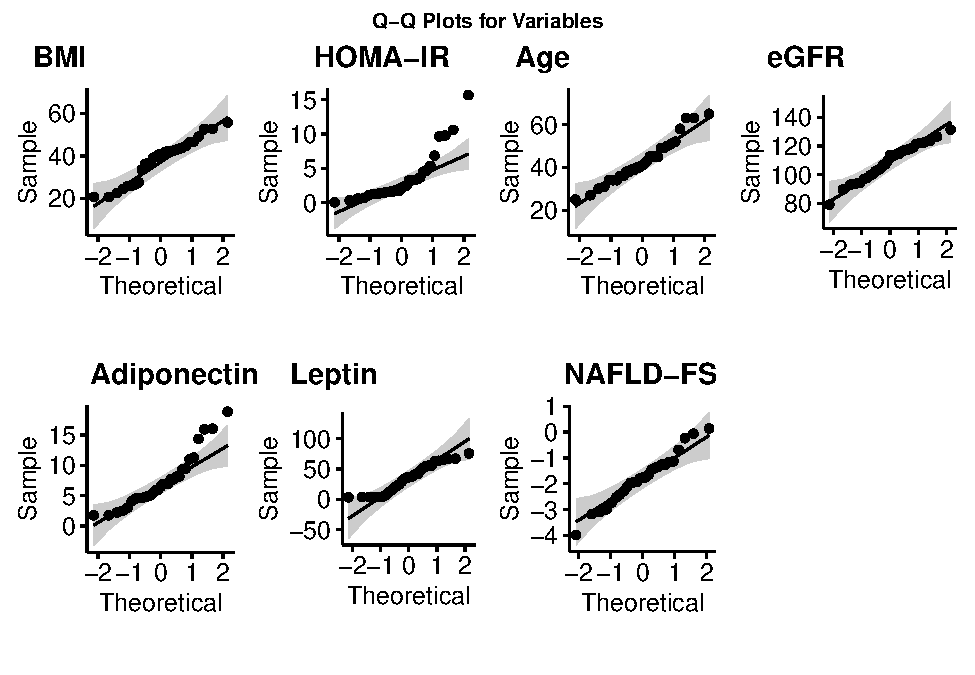
\includegraphics{StatisticalAnalysis_files/figure-latex/determine normality-1.pdf}

\global\setlength{\Oldarrayrulewidth}{\arrayrulewidth}

\global\setlength{\Oldtabcolsep}{\tabcolsep}

\setlength{\tabcolsep}{2pt}

\renewcommand*{\arraystretch}{1.5}



\providecommand{\ascline}[3]{\noalign{\global\arrayrulewidth #1}\arrayrulecolor[HTML]{#2}\cline{#3}}

\begin{longtable}[c]{cc}



\ascline{1.5pt}{666666}{1-2}

\multicolumn{2}{>{}c}{\textcolor[HTML]{000000}{\fontsize{11}{11}\selectfont{\global\setmainfont{Arial}{Shapiro-Wilk\ Normality\ Test}}}} \\

\ascline{1.5pt}{666666}{1-2}



\multicolumn{1}{>{}c}{\textcolor[HTML]{000000}{\fontsize{11}{11}\selectfont{\global\setmainfont{Arial}{Variable}}}} & \multicolumn{1}{>{}c}{\textcolor[HTML]{000000}{\fontsize{11}{11}\selectfont{\global\setmainfont{Arial}{p-value}}}} \\

\ascline{1.5pt}{666666}{1-2}\endfirsthead 

\ascline{1.5pt}{666666}{1-2}

\multicolumn{2}{>{}c}{\textcolor[HTML]{000000}{\fontsize{11}{11}\selectfont{\global\setmainfont{Arial}{Shapiro-Wilk\ Normality\ Test}}}} \\

\ascline{1.5pt}{666666}{1-2}



\multicolumn{1}{>{}c}{\textcolor[HTML]{000000}{\fontsize{11}{11}\selectfont{\global\setmainfont{Arial}{Variable}}}} & \multicolumn{1}{>{}c}{\textcolor[HTML]{000000}{\fontsize{11}{11}\selectfont{\global\setmainfont{Arial}{p-value}}}} \\

\ascline{1.5pt}{666666}{1-2}\endhead



\multicolumn{2}{>{}l}{\textcolor[HTML]{000000}{\fontsize{9}{9}\selectfont{\global\setmainfont{Arial}{Note:\ data\ with\ p-value<0.05\ will\ be\ log-transformed}}}} \\

\endlastfoot



\multicolumn{1}{>{}l}{\textcolor[HTML]{000000}{\fontsize{11}{11}\selectfont{\global\setmainfont{Arial}{BMI}}}} & \multicolumn{1}{>{}l}{\textcolor[HTML]{000000}{\fontsize{11}{11}\selectfont{\global\setmainfont{Arial}{0.078}}}} \\





\multicolumn{1}{>{}l}{\textcolor[HTML]{000000}{\fontsize{11}{11}\selectfont{\global\setmainfont{Arial}{HOMA-IR}}}} & \multicolumn{1}{>{}l}{\textcolor[HTML]{000000}{\fontsize{11}{11}\selectfont{\global\setmainfont{Arial}{1.56e-05}}}} \\





\multicolumn{1}{>{}l}{\textcolor[HTML]{000000}{\fontsize{11}{11}\selectfont{\global\setmainfont{Arial}{Age}}}} & \multicolumn{1}{>{}l}{\textcolor[HTML]{000000}{\fontsize{11}{11}\selectfont{\global\setmainfont{Arial}{0.274}}}} \\





\multicolumn{1}{>{}l}{\textcolor[HTML]{000000}{\fontsize{11}{11}\selectfont{\global\setmainfont{Arial}{eGFR}}}} & \multicolumn{1}{>{}l}{\textcolor[HTML]{000000}{\fontsize{11}{11}\selectfont{\global\setmainfont{Arial}{0.606}}}} \\





\multicolumn{1}{>{}l}{\textcolor[HTML]{000000}{\fontsize{11}{11}\selectfont{\global\setmainfont{Arial}{Adiponectin}}}} & \multicolumn{1}{>{}l}{\textcolor[HTML]{000000}{\fontsize{11}{11}\selectfont{\global\setmainfont{Arial}{0.008}}}} \\





\multicolumn{1}{>{}l}{\textcolor[HTML]{000000}{\fontsize{11}{11}\selectfont{\global\setmainfont{Arial}{Leptin}}}} & \multicolumn{1}{>{}l}{\textcolor[HTML]{000000}{\fontsize{11}{11}\selectfont{\global\setmainfont{Arial}{0.036}}}} \\





\multicolumn{1}{>{}l}{\textcolor[HTML]{000000}{\fontsize{11}{11}\selectfont{\global\setmainfont{Arial}{NAFLD-FS}}}} & \multicolumn{1}{>{}l}{\textcolor[HTML]{000000}{\fontsize{11}{11}\selectfont{\global\setmainfont{Arial}{0.927}}}} \\

\ascline{1.5pt}{666666}{1-2}



\end{longtable}



\arrayrulecolor[HTML]{000000}

\global\setlength{\arrayrulewidth}{\Oldarrayrulewidth}

\global\setlength{\tabcolsep}{\Oldtabcolsep}

\renewcommand*{\arraystretch}{1}

\newpage

\subsection{Determine Variable
Correlation}\label{determine-variable-correlation}

\global\setlength{\Oldarrayrulewidth}{\arrayrulewidth}

\global\setlength{\Oldtabcolsep}{\tabcolsep}

\setlength{\tabcolsep}{2pt}

\renewcommand*{\arraystretch}{1.5}



\providecommand{\ascline}[3]{\noalign{\global\arrayrulewidth #1}\arrayrulecolor[HTML]{#2}\cline{#3}}

\begin{longtable}[c]{|p{1.08in}|p{0.89in}}



\ascline{1.5pt}{666666}{1-2}

\multicolumn{2}{>{\centering}m{\dimexpr 1.97in+2\tabcolsep}}{\textcolor[HTML]{000000}{\fontsize{11}{11}\selectfont{\global\setmainfont{Arial}{ANOVA\ Results\ with\ Sex}}}} \\

\ascline{1.5pt}{666666}{1-2}



\multicolumn{1}{>{\centering}m{\dimexpr 1.08in+0\tabcolsep}}{\textcolor[HTML]{000000}{\fontsize{11}{11}\selectfont{\global\setmainfont{Arial}{Variable}}}} & \multicolumn{1}{>{\centering}m{\dimexpr 0.89in+0\tabcolsep}}{\textcolor[HTML]{000000}{\fontsize{11}{11}\selectfont{\global\setmainfont{Arial}{p-value}}}} \\

\ascline{1.5pt}{666666}{1-2}\endfirsthead 

\ascline{1.5pt}{666666}{1-2}

\multicolumn{2}{>{\centering}m{\dimexpr 1.97in+2\tabcolsep}}{\textcolor[HTML]{000000}{\fontsize{11}{11}\selectfont{\global\setmainfont{Arial}{ANOVA\ Results\ with\ Sex}}}} \\

\ascline{1.5pt}{666666}{1-2}



\multicolumn{1}{>{\centering}m{\dimexpr 1.08in+0\tabcolsep}}{\textcolor[HTML]{000000}{\fontsize{11}{11}\selectfont{\global\setmainfont{Arial}{Variable}}}} & \multicolumn{1}{>{\centering}m{\dimexpr 0.89in+0\tabcolsep}}{\textcolor[HTML]{000000}{\fontsize{11}{11}\selectfont{\global\setmainfont{Arial}{p-value}}}} \\

\ascline{1.5pt}{666666}{1-2}\endhead



\multicolumn{1}{>{\raggedright}m{\dimexpr 1.08in+0\tabcolsep}}{\textcolor[HTML]{000000}{\fontsize{11}{11}\selectfont{\global\setmainfont{Arial}{BMI}}}} & \multicolumn{1}{>{\raggedright}m{\dimexpr 0.89in+0\tabcolsep}}{\textcolor[HTML]{000000}{\fontsize{11}{11}\selectfont{\global\setmainfont{Arial}{8.04e-03}}}} \\





\multicolumn{1}{>{\raggedright}m{\dimexpr 1.08in+0\tabcolsep}}{\textcolor[HTML]{000000}{\fontsize{11}{11}\selectfont{\global\setmainfont{Arial}{HOMA-IR}}}} & \multicolumn{1}{>{\raggedright}m{\dimexpr 0.89in+0\tabcolsep}}{\textcolor[HTML]{000000}{\fontsize{11}{11}\selectfont{\global\setmainfont{Arial}{0.54}}}} \\





\multicolumn{1}{>{\raggedright}m{\dimexpr 1.08in+0\tabcolsep}}{\textcolor[HTML]{000000}{\fontsize{11}{11}\selectfont{\global\setmainfont{Arial}{Age}}}} & \multicolumn{1}{>{\raggedright}m{\dimexpr 0.89in+0\tabcolsep}}{\textcolor[HTML]{000000}{\fontsize{11}{11}\selectfont{\global\setmainfont{Arial}{0.59}}}} \\





\multicolumn{1}{>{\raggedright}m{\dimexpr 1.08in+0\tabcolsep}}{\textcolor[HTML]{000000}{\fontsize{11}{11}\selectfont{\global\setmainfont{Arial}{eGFR}}}} & \multicolumn{1}{>{\raggedright}m{\dimexpr 0.89in+0\tabcolsep}}{\textcolor[HTML]{000000}{\fontsize{11}{11}\selectfont{\global\setmainfont{Arial}{0.63}}}} \\





\multicolumn{1}{>{\raggedright}m{\dimexpr 1.08in+0\tabcolsep}}{\textcolor[HTML]{000000}{\fontsize{11}{11}\selectfont{\global\setmainfont{Arial}{Adiponectin}}}} & \multicolumn{1}{>{\raggedright}m{\dimexpr 0.89in+0\tabcolsep}}{\textcolor[HTML]{000000}{\fontsize{11}{11}\selectfont{\global\setmainfont{Arial}{0.92}}}} \\





\multicolumn{1}{>{\raggedright}m{\dimexpr 1.08in+0\tabcolsep}}{\textcolor[HTML]{000000}{\fontsize{11}{11}\selectfont{\global\setmainfont{Arial}{Leptin}}}} & \multicolumn{1}{>{\raggedright}m{\dimexpr 0.89in+0\tabcolsep}}{\textcolor[HTML]{000000}{\fontsize{11}{11}\selectfont{\global\setmainfont{Arial}{4.36e-05}}}} \\





\multicolumn{1}{>{\raggedright}m{\dimexpr 1.08in+0\tabcolsep}}{\textcolor[HTML]{000000}{\fontsize{11}{11}\selectfont{\global\setmainfont{Arial}{NAFLD-FS}}}} & \multicolumn{1}{>{\raggedright}m{\dimexpr 0.89in+0\tabcolsep}}{\textcolor[HTML]{000000}{\fontsize{11}{11}\selectfont{\global\setmainfont{Arial}{0.67}}}} \\

\ascline{1.5pt}{666666}{1-2}



\end{longtable}



\arrayrulecolor[HTML]{000000}

\global\setlength{\arrayrulewidth}{\Oldarrayrulewidth}

\global\setlength{\tabcolsep}{\Oldtabcolsep}

\renewcommand*{\arraystretch}{1}

\global\setlength{\Oldarrayrulewidth}{\arrayrulewidth}

\global\setlength{\Oldtabcolsep}{\tabcolsep}

\setlength{\tabcolsep}{2pt}

\renewcommand*{\arraystretch}{1.5}



\providecommand{\ascline}[3]{\noalign{\global\arrayrulewidth #1}\arrayrulecolor[HTML]{#2}\cline{#3}}

\begin{longtable}[c]{|p{2.09in}|p{0.63in}|p{0.89in}}



\ascline{1.5pt}{666666}{1-3}

\multicolumn{3}{>{\centering}m{\dimexpr 3.61in+4\tabcolsep}}{\textcolor[HTML]{000000}{\fontsize{11}{11}\selectfont{\global\setmainfont{Arial}{Spearman\ Correlation}}}} \\

\ascline{1.5pt}{666666}{1-3}



\multicolumn{1}{>{\centering}m{\dimexpr 2.09in+0\tabcolsep}}{\textcolor[HTML]{000000}{\fontsize{11}{11}\selectfont{\global\setmainfont{Arial}{Variable\ Pair}}}} & \multicolumn{1}{>{\centering}m{\dimexpr 0.63in+0\tabcolsep}}{\textcolor[HTML]{000000}{\fontsize{11}{11}\selectfont{\global\setmainfont{Arial}{rho}}}} & \multicolumn{1}{>{\centering}m{\dimexpr 0.89in+0\tabcolsep}}{\textcolor[HTML]{000000}{\fontsize{11}{11}\selectfont{\global\setmainfont{Arial}{p-value}}}} \\

\ascline{1.5pt}{666666}{1-3}\endfirsthead 

\ascline{1.5pt}{666666}{1-3}

\multicolumn{3}{>{\centering}m{\dimexpr 3.61in+4\tabcolsep}}{\textcolor[HTML]{000000}{\fontsize{11}{11}\selectfont{\global\setmainfont{Arial}{Spearman\ Correlation}}}} \\

\ascline{1.5pt}{666666}{1-3}



\multicolumn{1}{>{\centering}m{\dimexpr 2.09in+0\tabcolsep}}{\textcolor[HTML]{000000}{\fontsize{11}{11}\selectfont{\global\setmainfont{Arial}{Variable\ Pair}}}} & \multicolumn{1}{>{\centering}m{\dimexpr 0.63in+0\tabcolsep}}{\textcolor[HTML]{000000}{\fontsize{11}{11}\selectfont{\global\setmainfont{Arial}{rho}}}} & \multicolumn{1}{>{\centering}m{\dimexpr 0.89in+0\tabcolsep}}{\textcolor[HTML]{000000}{\fontsize{11}{11}\selectfont{\global\setmainfont{Arial}{p-value}}}} \\

\ascline{1.5pt}{666666}{1-3}\endhead



\multicolumn{1}{>{\raggedright}m{\dimexpr 2.09in+0\tabcolsep}}{\textcolor[HTML]{000000}{\fontsize{11}{11}\selectfont{\global\setmainfont{Arial}{BMI\ and\ Adiponectin}}}} & \multicolumn{1}{>{\raggedleft}m{\dimexpr 0.63in+0\tabcolsep}}{\textcolor[HTML]{000000}{\fontsize{11}{11}\selectfont{\global\setmainfont{Arial}{-0.35}}}} & \multicolumn{1}{>{\raggedright}m{\dimexpr 0.89in+0\tabcolsep}}{\textcolor[HTML]{000000}{\fontsize{11}{11}\selectfont{\global\setmainfont{Arial}{0.06}}}} \\





\multicolumn{1}{>{\raggedright}m{\dimexpr 2.09in+0\tabcolsep}}{\textcolor[HTML]{000000}{\fontsize{11}{11}\selectfont{\global\setmainfont{Arial}{BMI\ and\ Leptin}}}} & \multicolumn{1}{>{\raggedleft}m{\dimexpr 0.63in+0\tabcolsep}}{\textcolor[HTML]{000000}{\fontsize{11}{11}\selectfont{\global\setmainfont{Arial}{0.52}}}} & \multicolumn{1}{>{\raggedright}m{\dimexpr 0.89in+0\tabcolsep}}{\textcolor[HTML]{000000}{\fontsize{11}{11}\selectfont{\global\setmainfont{Arial}{2.94e-03}}}} \\





\multicolumn{1}{>{\raggedright}m{\dimexpr 2.09in+0\tabcolsep}}{\textcolor[HTML]{000000}{\fontsize{11}{11}\selectfont{\global\setmainfont{Arial}{HOMA-IR\ and\ Adiponectin}}}} & \multicolumn{1}{>{\raggedleft}m{\dimexpr 0.63in+0\tabcolsep}}{\textcolor[HTML]{000000}{\fontsize{11}{11}\selectfont{\global\setmainfont{Arial}{-0.59}}}} & \multicolumn{1}{>{\raggedright}m{\dimexpr 0.89in+0\tabcolsep}}{\textcolor[HTML]{000000}{\fontsize{11}{11}\selectfont{\global\setmainfont{Arial}{6.19e-04}}}} \\





\multicolumn{1}{>{\raggedright}m{\dimexpr 2.09in+0\tabcolsep}}{\textcolor[HTML]{000000}{\fontsize{11}{11}\selectfont{\global\setmainfont{Arial}{HOMA-IR\ and\ Leptin}}}} & \multicolumn{1}{>{\raggedleft}m{\dimexpr 0.63in+0\tabcolsep}}{\textcolor[HTML]{000000}{\fontsize{11}{11}\selectfont{\global\setmainfont{Arial}{0.25}}}} & \multicolumn{1}{>{\raggedright}m{\dimexpr 0.89in+0\tabcolsep}}{\textcolor[HTML]{000000}{\fontsize{11}{11}\selectfont{\global\setmainfont{Arial}{0.17}}}} \\

\ascline{1.5pt}{666666}{1-3}



\end{longtable}



\arrayrulecolor[HTML]{000000}

\global\setlength{\arrayrulewidth}{\Oldarrayrulewidth}

\global\setlength{\tabcolsep}{\Oldtabcolsep}

\renewcommand*{\arraystretch}{1}

\global\setlength{\Oldarrayrulewidth}{\arrayrulewidth}

\global\setlength{\Oldtabcolsep}{\tabcolsep}

\setlength{\tabcolsep}{2pt}

\renewcommand*{\arraystretch}{1.5}



\providecommand{\ascline}[3]{\noalign{\global\arrayrulewidth #1}\arrayrulecolor[HTML]{#2}\cline{#3}}

\begin{longtable}[c]{|p{1.55in}|p{0.79in}}



\ascline{1.5pt}{666666}{1-2}

\multicolumn{2}{>{\centering}m{\dimexpr 2.34in+2\tabcolsep}}{\textcolor[HTML]{000000}{\fontsize{11}{11}\selectfont{\global\setmainfont{Arial}{ANOVA\ Results}}}} \\

\ascline{1.5pt}{666666}{1-2}



\multicolumn{1}{>{\centering}m{\dimexpr 1.55in+0\tabcolsep}}{\textcolor[HTML]{000000}{\fontsize{11}{11}\selectfont{\global\setmainfont{Arial}{Variable\ Pair}}}} & \multicolumn{1}{>{\centering}m{\dimexpr 0.79in+0\tabcolsep}}{\textcolor[HTML]{000000}{\fontsize{11}{11}\selectfont{\global\setmainfont{Arial}{p-value}}}} \\

\ascline{1.5pt}{666666}{1-2}\endfirsthead 

\ascline{1.5pt}{666666}{1-2}

\multicolumn{2}{>{\centering}m{\dimexpr 2.34in+2\tabcolsep}}{\textcolor[HTML]{000000}{\fontsize{11}{11}\selectfont{\global\setmainfont{Arial}{ANOVA\ Results}}}} \\

\ascline{1.5pt}{666666}{1-2}



\multicolumn{1}{>{\centering}m{\dimexpr 1.55in+0\tabcolsep}}{\textcolor[HTML]{000000}{\fontsize{11}{11}\selectfont{\global\setmainfont{Arial}{Variable\ Pair}}}} & \multicolumn{1}{>{\centering}m{\dimexpr 0.79in+0\tabcolsep}}{\textcolor[HTML]{000000}{\fontsize{11}{11}\selectfont{\global\setmainfont{Arial}{p-value}}}} \\

\ascline{1.5pt}{666666}{1-2}\endhead



\multicolumn{2}{>{\raggedright}m{\dimexpr 2.34in+2\tabcolsep}}{\textcolor[HTML]{000000}{\fontsize{9}{9}\selectfont{\global\setmainfont{Arial}{Sex\ will\ be\ used\ for\ model\ building\ along\ with\ BMI,\ HOMA-IR,\ and\ Age}}}} \\

\endlastfoot



\multicolumn{1}{>{\raggedright}m{\dimexpr 1.55in+0\tabcolsep}}{\textcolor[HTML]{000000}{\fontsize{11}{11}\selectfont{\global\setmainfont{Arial}{BMI\ and\ Sex}}}} & \multicolumn{1}{>{\raggedleft}m{\dimexpr 0.79in+0\tabcolsep}}{\textcolor[HTML]{000000}{\fontsize{11}{11}\selectfont{\global\setmainfont{Arial}{0.008}}}} \\





\multicolumn{1}{>{\raggedright}m{\dimexpr 1.55in+0\tabcolsep}}{\textcolor[HTML]{000000}{\fontsize{11}{11}\selectfont{\global\setmainfont{Arial}{HOMA-IR\ and\ Sex}}}} & \multicolumn{1}{>{\raggedleft}m{\dimexpr 0.79in+0\tabcolsep}}{\textcolor[HTML]{000000}{\fontsize{11}{11}\selectfont{\global\setmainfont{Arial}{0.540}}}} \\





\multicolumn{1}{>{\raggedright}m{\dimexpr 1.55in+0\tabcolsep}}{\textcolor[HTML]{000000}{\fontsize{11}{11}\selectfont{\global\setmainfont{Arial}{Age\ and\ Sex}}}} & \multicolumn{1}{>{\raggedleft}m{\dimexpr 0.79in+0\tabcolsep}}{\textcolor[HTML]{000000}{\fontsize{11}{11}\selectfont{\global\setmainfont{Arial}{0.587}}}} \\

\ascline{1.5pt}{666666}{1-2}



\end{longtable}



\arrayrulecolor[HTML]{000000}

\global\setlength{\arrayrulewidth}{\Oldarrayrulewidth}

\global\setlength{\tabcolsep}{\Oldtabcolsep}

\renewcommand*{\arraystretch}{1}

\global\setlength{\Oldarrayrulewidth}{\arrayrulewidth}

\global\setlength{\Oldtabcolsep}{\tabcolsep}

\setlength{\tabcolsep}{2pt}

\renewcommand*{\arraystretch}{1.5}



\providecommand{\ascline}[3]{\noalign{\global\arrayrulewidth #1}\arrayrulecolor[HTML]{#2}\cline{#3}}

\begin{longtable}[c]{|p{1.56in}|p{0.63in}|p{0.79in}}



\ascline{1.5pt}{666666}{1-3}

\multicolumn{3}{>{\centering}m{\dimexpr 2.98in+4\tabcolsep}}{\textcolor[HTML]{000000}{\fontsize{11}{11}\selectfont{\global\setmainfont{Arial}{Spearman\ Correlation}}}} \\

\ascline{1.5pt}{666666}{1-3}



\multicolumn{1}{>{\centering}m{\dimexpr 1.56in+0\tabcolsep}}{\textcolor[HTML]{000000}{\fontsize{11}{11}\selectfont{\global\setmainfont{Arial}{Variable\ Pair}}}} & \multicolumn{1}{>{\centering}m{\dimexpr 0.63in+0\tabcolsep}}{\textcolor[HTML]{000000}{\fontsize{11}{11}\selectfont{\global\setmainfont{Arial}{rho}}}} & \multicolumn{1}{>{\centering}m{\dimexpr 0.79in+0\tabcolsep}}{\textcolor[HTML]{000000}{\fontsize{11}{11}\selectfont{\global\setmainfont{Arial}{p-value}}}} \\

\ascline{1.5pt}{666666}{1-3}\endfirsthead 

\ascline{1.5pt}{666666}{1-3}

\multicolumn{3}{>{\centering}m{\dimexpr 2.98in+4\tabcolsep}}{\textcolor[HTML]{000000}{\fontsize{11}{11}\selectfont{\global\setmainfont{Arial}{Spearman\ Correlation}}}} \\

\ascline{1.5pt}{666666}{1-3}



\multicolumn{1}{>{\centering}m{\dimexpr 1.56in+0\tabcolsep}}{\textcolor[HTML]{000000}{\fontsize{11}{11}\selectfont{\global\setmainfont{Arial}{Variable\ Pair}}}} & \multicolumn{1}{>{\centering}m{\dimexpr 0.63in+0\tabcolsep}}{\textcolor[HTML]{000000}{\fontsize{11}{11}\selectfont{\global\setmainfont{Arial}{rho}}}} & \multicolumn{1}{>{\centering}m{\dimexpr 0.79in+0\tabcolsep}}{\textcolor[HTML]{000000}{\fontsize{11}{11}\selectfont{\global\setmainfont{Arial}{p-value}}}} \\

\ascline{1.5pt}{666666}{1-3}\endhead



\multicolumn{3}{>{\raggedright}m{\dimexpr 2.98in+4\tabcolsep}}{\textcolor[HTML]{000000}{\fontsize{9}{9}\selectfont{\global\setmainfont{Arial}{These\ variables\ will\ be\ used\ for\ model\ building\ along\ with\ the\ variable\ Sex}}}} \\

\endlastfoot



\multicolumn{1}{>{\raggedright}m{\dimexpr 1.56in+0\tabcolsep}}{\textcolor[HTML]{000000}{\fontsize{11}{11}\selectfont{\global\setmainfont{Arial}{BMI\ and\ Age}}}} & \multicolumn{1}{>{\raggedleft}m{\dimexpr 0.63in+0\tabcolsep}}{\textcolor[HTML]{000000}{\fontsize{11}{11}\selectfont{\global\setmainfont{Arial}{-0.37}}}} & \multicolumn{1}{>{\raggedleft}m{\dimexpr 0.79in+0\tabcolsep}}{\textcolor[HTML]{000000}{\fontsize{11}{11}\selectfont{\global\setmainfont{Arial}{0.042}}}} \\





\multicolumn{1}{>{\raggedright}m{\dimexpr 1.56in+0\tabcolsep}}{\textcolor[HTML]{000000}{\fontsize{11}{11}\selectfont{\global\setmainfont{Arial}{BMI\ and\ HOMA-IR}}}} & \multicolumn{1}{>{\raggedleft}m{\dimexpr 0.63in+0\tabcolsep}}{\textcolor[HTML]{000000}{\fontsize{11}{11}\selectfont{\global\setmainfont{Arial}{0.52}}}} & \multicolumn{1}{>{\raggedleft}m{\dimexpr 0.79in+0\tabcolsep}}{\textcolor[HTML]{000000}{\fontsize{11}{11}\selectfont{\global\setmainfont{Arial}{0.003}}}} \\





\multicolumn{1}{>{\raggedright}m{\dimexpr 1.56in+0\tabcolsep}}{\textcolor[HTML]{000000}{\fontsize{11}{11}\selectfont{\global\setmainfont{Arial}{Age\ and\ HOMA-IR}}}} & \multicolumn{1}{>{\raggedleft}m{\dimexpr 0.63in+0\tabcolsep}}{\textcolor[HTML]{000000}{\fontsize{11}{11}\selectfont{\global\setmainfont{Arial}{-0.41}}}} & \multicolumn{1}{>{\raggedleft}m{\dimexpr 0.79in+0\tabcolsep}}{\textcolor[HTML]{000000}{\fontsize{11}{11}\selectfont{\global\setmainfont{Arial}{0.022}}}} \\

\ascline{1.5pt}{666666}{1-3}



\end{longtable}



\arrayrulecolor[HTML]{000000}

\global\setlength{\arrayrulewidth}{\Oldarrayrulewidth}

\global\setlength{\tabcolsep}{\Oldtabcolsep}

\renewcommand*{\arraystretch}{1}

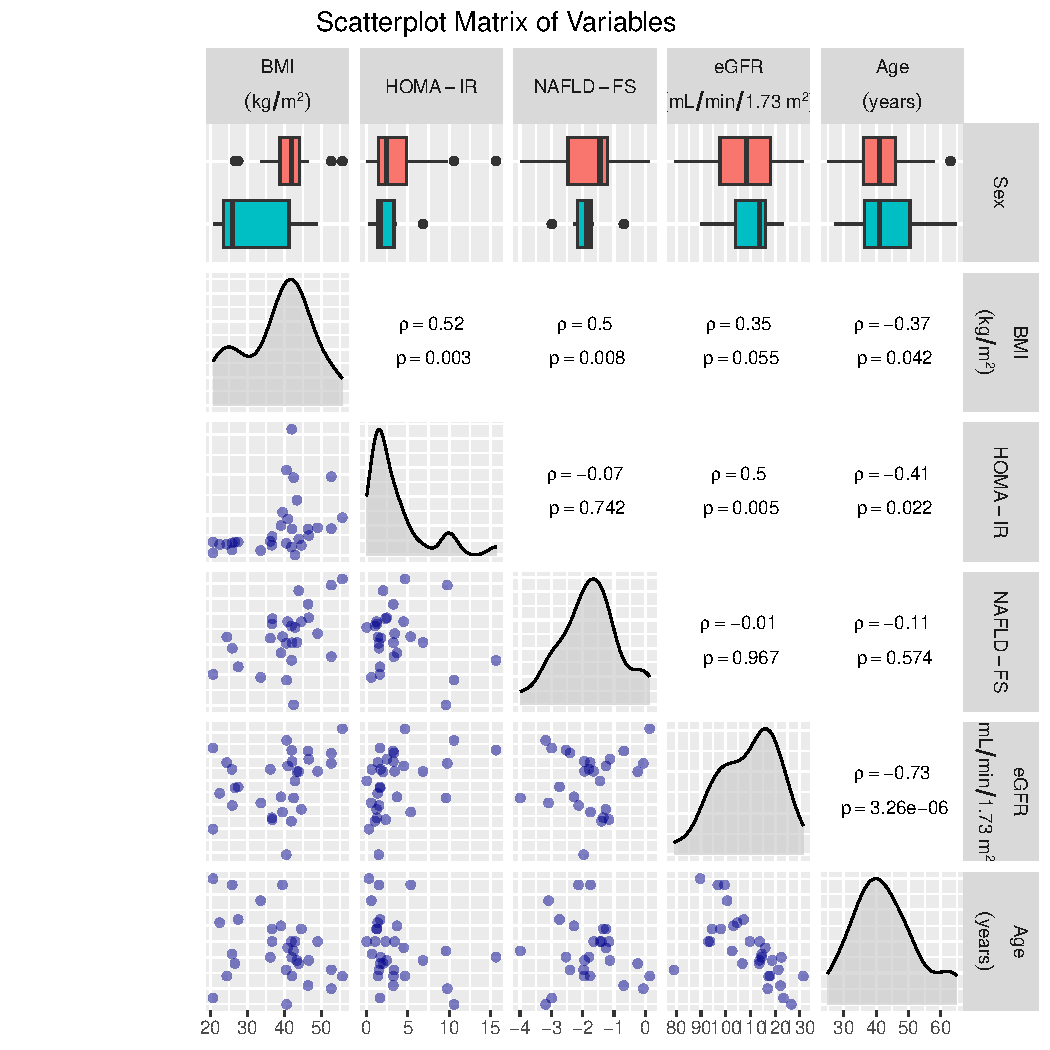
\includegraphics{StatisticalAnalysis_files/figure-latex/variable matrix-1.pdf}

\newpage

\section{RBP4 Model}\label{rbp4-model}

\begin{Shaded}
\begin{Highlighting}[]
\CommentTok{\#log transform RBP4 concentrations}
\NormalTok{vao}\SpecialCharTok{$}\NormalTok{LRBP4}\OtherTok{\textless{}{-}}\FunctionTok{log10}\NormalTok{(vao}\SpecialCharTok{$}\NormalTok{RBP4)}

\CommentTok{\#linear regression with BMI, Sex, Age and HOMAIR}
\NormalTok{model1}\OtherTok{=}\FunctionTok{lm}\NormalTok{(LRBP4}\SpecialCharTok{\textasciitilde{}}\NormalTok{BMI}\SpecialCharTok{+}\NormalTok{Sex}\SpecialCharTok{+}\NormalTok{Age}\SpecialCharTok{+}\NormalTok{LHOMAIR,vao)}
\FunctionTok{vif}\NormalTok{(model1)}
\end{Highlighting}
\end{Shaded}

\begin{verbatim}
##      BMI      Sex      Age  LHOMAIR 
## 1.597502 1.292650 1.233974 1.259206
\end{verbatim}

\begin{Shaded}
\begin{Highlighting}[]
\CommentTok{\#remove one variable at a time}
\NormalTok{model2}\OtherTok{=}\FunctionTok{lm}\NormalTok{(LRBP4}\SpecialCharTok{\textasciitilde{}}\NormalTok{BMI}\SpecialCharTok{+}\NormalTok{Sex}\SpecialCharTok{+}\NormalTok{Age,vao) }\CommentTok{\#remove HOMAIR}
\NormalTok{model3}\OtherTok{=}\FunctionTok{lm}\NormalTok{(LRBP4}\SpecialCharTok{\textasciitilde{}}\NormalTok{BMI}\SpecialCharTok{+}\NormalTok{Sex}\SpecialCharTok{+}\NormalTok{LHOMAIR, vao) }\CommentTok{\#remove Age}
\NormalTok{model4}\OtherTok{=}\FunctionTok{lm}\NormalTok{(LRBP4}\SpecialCharTok{\textasciitilde{}}\NormalTok{BMI}\SpecialCharTok{+}\NormalTok{Age}\SpecialCharTok{+}\NormalTok{LHOMAIR, vao) }\CommentTok{\#remove Sex}
\NormalTok{model5}\OtherTok{=}\FunctionTok{lm}\NormalTok{(LRBP4}\SpecialCharTok{\textasciitilde{}}\NormalTok{Sex}\SpecialCharTok{+}\NormalTok{Age}\SpecialCharTok{+}\NormalTok{LHOMAIR, vao) }\CommentTok{\#remove BMI}

\NormalTok{AIC}\OtherTok{\textless{}{-}}\FunctionTok{AIC}\NormalTok{(model1,model2,model3,model4,model5) }\CommentTok{\#summary of AIC}
\NormalTok{AIC\_df}\OtherTok{\textless{}{-}}\FunctionTok{data.frame}\NormalTok{(}
  \AttributeTok{Model=}\FunctionTok{c}\NormalTok{(}\StringTok{"Model 1: Full Model"}\NormalTok{, }\StringTok{"Model 2: No HOMA{-}IR"}\NormalTok{, }\StringTok{"Model 3: No Age"}\NormalTok{,}
          \StringTok{"Model 4: No Sex"}\NormalTok{, }\StringTok{"Model 5: No BMI"}\NormalTok{),}
  \AttributeTok{AIC =} \FunctionTok{round}\NormalTok{(AIC}\SpecialCharTok{$}\NormalTok{AIC, }\DecValTok{3}\NormalTok{),}
  \AttributeTok{DF =}\NormalTok{ AIC}\SpecialCharTok{$}\NormalTok{df)}

\NormalTok{aic\_table }\OtherTok{\textless{}{-}}\NormalTok{ AIC\_df }\SpecialCharTok{\%\textgreater{}\%}
  \FunctionTok{flextable}\NormalTok{() }\SpecialCharTok{\%\textgreater{}\%}
  \FunctionTok{set\_header\_labels}\NormalTok{(}\AttributeTok{Model =} \StringTok{"Model Description"}\NormalTok{, }\AttributeTok{AIC =} \StringTok{"AIC Value"}\NormalTok{,}
                    \AttributeTok{DF=}\StringTok{"Degrees of Freedom"}\NormalTok{) }\SpecialCharTok{\%\textgreater{}\%}
  \FunctionTok{add\_header\_lines}\NormalTok{(}\AttributeTok{values =} \StringTok{"AIC Comparison of Models"}\NormalTok{) }\SpecialCharTok{\%\textgreater{}\%}
  \FunctionTok{align}\NormalTok{(}\AttributeTok{part=}\StringTok{"header"}\NormalTok{, }\AttributeTok{align=}\StringTok{"center"}\NormalTok{ ) }\SpecialCharTok{\%\textgreater{}\%}
  \FunctionTok{add\_footer\_lines}\NormalTok{(}\AttributeTok{values =} \StringTok{"Note: Lower AIC values indicate a better model."}\NormalTok{) }\SpecialCharTok{\%\textgreater{}\%}
  \FunctionTok{fontsize}\NormalTok{(}\AttributeTok{part =} \StringTok{"footer"}\NormalTok{, }\AttributeTok{size =} \DecValTok{8}\NormalTok{) }\SpecialCharTok{\%\textgreater{}\%}
  \FunctionTok{set\_table\_properties}\NormalTok{(}\AttributeTok{layout =} \StringTok{"autofit"}\NormalTok{)}
\NormalTok{aic\_table}
\end{Highlighting}
\end{Shaded}

\global\setlength{\Oldarrayrulewidth}{\arrayrulewidth}

\global\setlength{\Oldtabcolsep}{\tabcolsep}

\setlength{\tabcolsep}{2pt}

\renewcommand*{\arraystretch}{1.5}



\providecommand{\ascline}[3]{\noalign{\global\arrayrulewidth #1}\arrayrulecolor[HTML]{#2}\cline{#3}}

\begin{longtable}[c]{ccc}



\ascline{1.5pt}{666666}{1-3}

\multicolumn{3}{>{}c}{\textcolor[HTML]{000000}{\fontsize{11}{11}\selectfont{\global\setmainfont{Arial}{AIC\ Comparison\ of\ Models}}}} \\

\ascline{1.5pt}{666666}{1-3}



\multicolumn{1}{>{}c}{\textcolor[HTML]{000000}{\fontsize{11}{11}\selectfont{\global\setmainfont{Arial}{Model\ Description}}}} & \multicolumn{1}{>{}c}{\textcolor[HTML]{000000}{\fontsize{11}{11}\selectfont{\global\setmainfont{Arial}{AIC\ Value}}}} & \multicolumn{1}{>{}c}{\textcolor[HTML]{000000}{\fontsize{11}{11}\selectfont{\global\setmainfont{Arial}{Degrees\ of\ Freedom}}}} \\

\ascline{1.5pt}{666666}{1-3}\endfirsthead 

\ascline{1.5pt}{666666}{1-3}

\multicolumn{3}{>{}c}{\textcolor[HTML]{000000}{\fontsize{11}{11}\selectfont{\global\setmainfont{Arial}{AIC\ Comparison\ of\ Models}}}} \\

\ascline{1.5pt}{666666}{1-3}



\multicolumn{1}{>{}c}{\textcolor[HTML]{000000}{\fontsize{11}{11}\selectfont{\global\setmainfont{Arial}{Model\ Description}}}} & \multicolumn{1}{>{}c}{\textcolor[HTML]{000000}{\fontsize{11}{11}\selectfont{\global\setmainfont{Arial}{AIC\ Value}}}} & \multicolumn{1}{>{}c}{\textcolor[HTML]{000000}{\fontsize{11}{11}\selectfont{\global\setmainfont{Arial}{Degrees\ of\ Freedom}}}} \\

\ascline{1.5pt}{666666}{1-3}\endhead



\multicolumn{3}{>{}l}{\textcolor[HTML]{000000}{\fontsize{8}{8}\selectfont{\global\setmainfont{Arial}{Note:\ Lower\ AIC\ values\ indicate\ a\ better\ model.}}}} \\

\endlastfoot



\multicolumn{1}{>{}l}{\textcolor[HTML]{000000}{\fontsize{11}{11}\selectfont{\global\setmainfont{Arial}{Model\ 1:\ Full\ Model}}}} & \multicolumn{1}{>{}r}{\textcolor[HTML]{000000}{\fontsize{11}{11}\selectfont{\global\setmainfont{Arial}{-34.866}}}} & \multicolumn{1}{>{}r}{\textcolor[HTML]{000000}{\fontsize{11}{11}\selectfont{\global\setmainfont{Arial}{6}}}} \\





\multicolumn{1}{>{}l}{\textcolor[HTML]{000000}{\fontsize{11}{11}\selectfont{\global\setmainfont{Arial}{Model\ 2:\ No\ HOMA-IR}}}} & \multicolumn{1}{>{}r}{\textcolor[HTML]{000000}{\fontsize{11}{11}\selectfont{\global\setmainfont{Arial}{-36.135}}}} & \multicolumn{1}{>{}r}{\textcolor[HTML]{000000}{\fontsize{11}{11}\selectfont{\global\setmainfont{Arial}{5}}}} \\





\multicolumn{1}{>{}l}{\textcolor[HTML]{000000}{\fontsize{11}{11}\selectfont{\global\setmainfont{Arial}{Model\ 3:\ No\ Age}}}} & \multicolumn{1}{>{}r}{\textcolor[HTML]{000000}{\fontsize{11}{11}\selectfont{\global\setmainfont{Arial}{-35.123}}}} & \multicolumn{1}{>{}r}{\textcolor[HTML]{000000}{\fontsize{11}{11}\selectfont{\global\setmainfont{Arial}{5}}}} \\





\multicolumn{1}{>{}l}{\textcolor[HTML]{000000}{\fontsize{11}{11}\selectfont{\global\setmainfont{Arial}{Model\ 4:\ No\ Sex}}}} & \multicolumn{1}{>{}r}{\textcolor[HTML]{000000}{\fontsize{11}{11}\selectfont{\global\setmainfont{Arial}{-33.703}}}} & \multicolumn{1}{>{}r}{\textcolor[HTML]{000000}{\fontsize{11}{11}\selectfont{\global\setmainfont{Arial}{5}}}} \\





\multicolumn{1}{>{}l}{\textcolor[HTML]{000000}{\fontsize{11}{11}\selectfont{\global\setmainfont{Arial}{Model\ 5:\ No\ BMI}}}} & \multicolumn{1}{>{}r}{\textcolor[HTML]{000000}{\fontsize{11}{11}\selectfont{\global\setmainfont{Arial}{-36.196}}}} & \multicolumn{1}{>{}r}{\textcolor[HTML]{000000}{\fontsize{11}{11}\selectfont{\global\setmainfont{Arial}{5}}}} \\

\ascline{1.5pt}{666666}{1-3}



\end{longtable}



\arrayrulecolor[HTML]{000000}

\global\setlength{\arrayrulewidth}{\Oldarrayrulewidth}

\global\setlength{\tabcolsep}{\Oldtabcolsep}

\renewcommand*{\arraystretch}{1}

\begin{Shaded}
\begin{Highlighting}[]
\DocumentationTok{\#\#remove BMI (lowest AIC), add interaction terms}
\NormalTok{model6}\OtherTok{=}\FunctionTok{lm}\NormalTok{(LRBP4}\SpecialCharTok{\textasciitilde{}}\NormalTok{Sex}\SpecialCharTok{+}\NormalTok{Age}\SpecialCharTok{+}\NormalTok{LHOMAIR}\SpecialCharTok{+}\NormalTok{Age}\SpecialCharTok{*}\NormalTok{Sex}\SpecialCharTok{+}\NormalTok{LHOMAIR}\SpecialCharTok{*}\NormalTok{Sex,vao)}
\FunctionTok{summary}\NormalTok{(model6)}
\end{Highlighting}
\end{Shaded}

\begin{verbatim}
## 
## Call:
## lm(formula = LRBP4 ~ Sex + Age + LHOMAIR + Age * Sex + LHOMAIR * 
##     Sex, data = vao)
## 
## Residuals:
##      Min       1Q   Median       3Q      Max 
## -0.21429 -0.07825  0.02313  0.06886  0.20592 
## 
## Coefficients:
##                  Estimate Std. Error t value Pr(>|t|)   
## (Intercept)     -0.071668   0.135146  -0.530  0.60058   
## SexMale          0.507136   0.207240   2.447  0.02177 * 
## Age              0.008636   0.002998   2.880  0.00803 **
## LHOMAIR         -0.048056   0.045468  -1.057  0.30065   
## SexMale:Age     -0.009698   0.004385  -2.212  0.03636 * 
## SexMale:LHOMAIR  0.072444   0.113449   0.639  0.52892   
## ---
## Signif. codes:  0 '***' 0.001 '**' 0.01 '*' 0.05 '.' 0.1 ' ' 1
## 
## Residual standard error: 0.1123 on 25 degrees of freedom
## Multiple R-squared:  0.4636, Adjusted R-squared:  0.3563 
## F-statistic: 4.322 on 5 and 25 DF,  p-value: 0.005699
\end{verbatim}

\begin{Shaded}
\begin{Highlighting}[]
\FunctionTok{AIC}\NormalTok{(model6,model5)}
\end{Highlighting}
\end{Shaded}

\begin{longtable}[]{@{}lrr@{}}
\toprule\noalign{}
& df & AIC \\
\midrule\noalign{}
\endhead
\bottomrule\noalign{}
\endlastfoot
model6 & 7 & -40.24879 \\
model5 & 5 & -36.19628 \\
\end{longtable}

\begin{Shaded}
\begin{Highlighting}[]
\CommentTok{\#remove interaction terms one at a time}
\NormalTok{model7}\OtherTok{=}\FunctionTok{lm}\NormalTok{(LRBP4}\SpecialCharTok{\textasciitilde{}}\NormalTok{Sex}\SpecialCharTok{+}\NormalTok{Age}\SpecialCharTok{+}\NormalTok{LHOMAIR}\SpecialCharTok{+}\NormalTok{LHOMAIR}\SpecialCharTok{*}\NormalTok{Age,vao)}
\NormalTok{model8}\OtherTok{=}\FunctionTok{lm}\NormalTok{(LRBP4}\SpecialCharTok{\textasciitilde{}}\NormalTok{Sex}\SpecialCharTok{+}\NormalTok{Age}\SpecialCharTok{+}\NormalTok{LHOMAIR}\SpecialCharTok{+}\NormalTok{Age}\SpecialCharTok{*}\NormalTok{Sex,vao)}
\FunctionTok{summary}\NormalTok{(model7)}
\end{Highlighting}
\end{Shaded}

\begin{verbatim}
## 
## Call:
## lm(formula = LRBP4 ~ Sex + Age + LHOMAIR + LHOMAIR * Age, data = vao)
## 
## Residuals:
##      Min       1Q   Median       3Q      Max 
## -0.24923 -0.06776  0.01125  0.07561  0.20708 
## 
## Coefficients:
##              Estimate Std. Error t value Pr(>|t|)  
## (Intercept)  0.183427   0.135373   1.355   0.1871  
## SexMale      0.106354   0.047271   2.250   0.0331 *
## Age          0.002726   0.002839   0.960   0.3458  
## LHOMAIR     -0.156739   0.218925  -0.716   0.4804  
## Age:LHOMAIR  0.002452   0.004827   0.508   0.6157  
## ---
## Signif. codes:  0 '***' 0.001 '**' 0.01 '*' 0.05 '.' 0.1 ' ' 1
## 
## Residual standard error: 0.1248 on 26 degrees of freedom
## Multiple R-squared:  0.3113, Adjusted R-squared:  0.2054 
## F-statistic: 2.939 on 4 and 26 DF,  p-value: 0.03955
\end{verbatim}

\begin{Shaded}
\begin{Highlighting}[]
\FunctionTok{summary}\NormalTok{(model8)}
\end{Highlighting}
\end{Shaded}

\begin{verbatim}
## 
## Call:
## lm(formula = LRBP4 ~ Sex + Age + LHOMAIR + Age * Sex, data = vao)
## 
## Residuals:
##      Min       1Q   Median       3Q      Max 
## -0.21447 -0.05720  0.02090  0.07151  0.20229 
## 
## Coefficients:
##              Estimate Std. Error t value Pr(>|t|)   
## (Intercept) -0.087232   0.131407  -0.664  0.51264   
## SexMale      0.571891   0.178663   3.201  0.00359 **
## Age          0.008906   0.002934   3.035  0.00541 **
## LHOMAIR     -0.036421   0.041179  -0.884  0.38456   
## SexMale:Age -0.010753   0.004015  -2.678  0.01267 * 
## ---
## Signif. codes:  0 '***' 0.001 '**' 0.01 '*' 0.05 '.' 0.1 ' ' 1
## 
## Residual standard error: 0.111 on 26 degrees of freedom
## Multiple R-squared:  0.4549, Adjusted R-squared:  0.371 
## F-statistic: 5.424 on 4 and 26 DF,  p-value: 0.002596
\end{verbatim}

\begin{Shaded}
\begin{Highlighting}[]
\FunctionTok{AIC}\NormalTok{(model6,model7,model8) }\CommentTok{\#remove HOMAIR x Age }
\end{Highlighting}
\end{Shaded}

\begin{longtable}[]{@{}lrr@{}}
\toprule\noalign{}
& df & AIC \\
\midrule\noalign{}
\endhead
\bottomrule\noalign{}
\endlastfoot
model6 & 7 & -40.24879 \\
model7 & 6 & -34.50246 \\
model8 & 6 & -41.74725 \\
\end{longtable}

\begin{Shaded}
\begin{Highlighting}[]
\NormalTok{AIC\_RBP4\_iterm}\OtherTok{\textless{}{-}}\FunctionTok{AIC}\NormalTok{(model6,model7,model8) }\CommentTok{\#summary of AIC}
\NormalTok{AIC\_df\_RBP4\_iterm}\OtherTok{\textless{}{-}}\FunctionTok{data.frame}\NormalTok{(}
  \AttributeTok{Model=}\FunctionTok{c}\NormalTok{(}\StringTok{"Model 6: Includes interaction terms"}\NormalTok{, }\StringTok{"Model 7: Remove Age x Sex"}\NormalTok{, }
          \StringTok{"Model 8: Remove HOMA{-}IR x Sex"}\NormalTok{),}
  \AttributeTok{AIC =} \FunctionTok{round}\NormalTok{(AIC\_RBP4\_iterm}\SpecialCharTok{$}\NormalTok{AIC,}\DecValTok{3}\NormalTok{),}
  \AttributeTok{DF =}\NormalTok{ AIC\_RBP4\_iterm}\SpecialCharTok{$}\NormalTok{df)}

\NormalTok{aic\_RBP4\_iterm\_table }\OtherTok{\textless{}{-}}\NormalTok{ AIC\_df\_RBP4\_iterm }\SpecialCharTok{\%\textgreater{}\%}
  \FunctionTok{flextable}\NormalTok{() }\SpecialCharTok{\%\textgreater{}\%}
  \FunctionTok{set\_header\_labels}\NormalTok{(}\AttributeTok{Model =} \StringTok{"Model Description"}\NormalTok{, }\AttributeTok{AIC =} \StringTok{"AIC Value"}\NormalTok{,}
                    \AttributeTok{DF=}\StringTok{"Degrees of Freedom"}\NormalTok{) }\SpecialCharTok{\%\textgreater{}\%}
  \FunctionTok{add\_header\_lines}\NormalTok{(}\AttributeTok{values =} \StringTok{"AIC Comparison of Models"}\NormalTok{) }\SpecialCharTok{\%\textgreater{}\%}
  \FunctionTok{align}\NormalTok{(}\AttributeTok{part=}\StringTok{"header"}\NormalTok{, }\AttributeTok{align=}\StringTok{"center"}\NormalTok{ ) }\SpecialCharTok{\%\textgreater{}\%}
  \FunctionTok{add\_footer\_lines}\NormalTok{(}\AttributeTok{values =} \StringTok{"Note: Lower AIC values indicate a better model."}\NormalTok{) }\SpecialCharTok{\%\textgreater{}\%}
  \FunctionTok{fontsize}\NormalTok{(}\AttributeTok{part =} \StringTok{"footer"}\NormalTok{, }\AttributeTok{size =} \DecValTok{8}\NormalTok{) }\SpecialCharTok{\%\textgreater{}\%}
  \FunctionTok{set\_table\_properties}\NormalTok{(}\AttributeTok{layout =} \StringTok{"autofit"}\NormalTok{)}
\NormalTok{aic\_RBP4\_iterm\_table}
\end{Highlighting}
\end{Shaded}

\global\setlength{\Oldarrayrulewidth}{\arrayrulewidth}

\global\setlength{\Oldtabcolsep}{\tabcolsep}

\setlength{\tabcolsep}{2pt}

\renewcommand*{\arraystretch}{1.5}



\providecommand{\ascline}[3]{\noalign{\global\arrayrulewidth #1}\arrayrulecolor[HTML]{#2}\cline{#3}}

\begin{longtable}[c]{ccc}



\ascline{1.5pt}{666666}{1-3}

\multicolumn{3}{>{}c}{\textcolor[HTML]{000000}{\fontsize{11}{11}\selectfont{\global\setmainfont{Arial}{AIC\ Comparison\ of\ Models}}}} \\

\ascline{1.5pt}{666666}{1-3}



\multicolumn{1}{>{}c}{\textcolor[HTML]{000000}{\fontsize{11}{11}\selectfont{\global\setmainfont{Arial}{Model\ Description}}}} & \multicolumn{1}{>{}c}{\textcolor[HTML]{000000}{\fontsize{11}{11}\selectfont{\global\setmainfont{Arial}{AIC\ Value}}}} & \multicolumn{1}{>{}c}{\textcolor[HTML]{000000}{\fontsize{11}{11}\selectfont{\global\setmainfont{Arial}{Degrees\ of\ Freedom}}}} \\

\ascline{1.5pt}{666666}{1-3}\endfirsthead 

\ascline{1.5pt}{666666}{1-3}

\multicolumn{3}{>{}c}{\textcolor[HTML]{000000}{\fontsize{11}{11}\selectfont{\global\setmainfont{Arial}{AIC\ Comparison\ of\ Models}}}} \\

\ascline{1.5pt}{666666}{1-3}



\multicolumn{1}{>{}c}{\textcolor[HTML]{000000}{\fontsize{11}{11}\selectfont{\global\setmainfont{Arial}{Model\ Description}}}} & \multicolumn{1}{>{}c}{\textcolor[HTML]{000000}{\fontsize{11}{11}\selectfont{\global\setmainfont{Arial}{AIC\ Value}}}} & \multicolumn{1}{>{}c}{\textcolor[HTML]{000000}{\fontsize{11}{11}\selectfont{\global\setmainfont{Arial}{Degrees\ of\ Freedom}}}} \\

\ascline{1.5pt}{666666}{1-3}\endhead



\multicolumn{3}{>{}l}{\textcolor[HTML]{000000}{\fontsize{8}{8}\selectfont{\global\setmainfont{Arial}{Note:\ Lower\ AIC\ values\ indicate\ a\ better\ model.}}}} \\

\endlastfoot



\multicolumn{1}{>{}l}{\textcolor[HTML]{000000}{\fontsize{11}{11}\selectfont{\global\setmainfont{Arial}{Model\ 6:\ Includes\ interaction\ terms}}}} & \multicolumn{1}{>{}r}{\textcolor[HTML]{000000}{\fontsize{11}{11}\selectfont{\global\setmainfont{Arial}{-40.249}}}} & \multicolumn{1}{>{}r}{\textcolor[HTML]{000000}{\fontsize{11}{11}\selectfont{\global\setmainfont{Arial}{7}}}} \\





\multicolumn{1}{>{}l}{\textcolor[HTML]{000000}{\fontsize{11}{11}\selectfont{\global\setmainfont{Arial}{Model\ 7:\ Remove\ Age\ x\ Sex}}}} & \multicolumn{1}{>{}r}{\textcolor[HTML]{000000}{\fontsize{11}{11}\selectfont{\global\setmainfont{Arial}{-34.502}}}} & \multicolumn{1}{>{}r}{\textcolor[HTML]{000000}{\fontsize{11}{11}\selectfont{\global\setmainfont{Arial}{6}}}} \\





\multicolumn{1}{>{}l}{\textcolor[HTML]{000000}{\fontsize{11}{11}\selectfont{\global\setmainfont{Arial}{Model\ 8:\ Remove\ HOMA-IR\ x\ Sex}}}} & \multicolumn{1}{>{}r}{\textcolor[HTML]{000000}{\fontsize{11}{11}\selectfont{\global\setmainfont{Arial}{-41.747}}}} & \multicolumn{1}{>{}r}{\textcolor[HTML]{000000}{\fontsize{11}{11}\selectfont{\global\setmainfont{Arial}{6}}}} \\

\ascline{1.5pt}{666666}{1-3}



\end{longtable}



\arrayrulecolor[HTML]{000000}

\global\setlength{\arrayrulewidth}{\Oldarrayrulewidth}

\global\setlength{\tabcolsep}{\Oldtabcolsep}

\renewcommand*{\arraystretch}{1}

\begin{Shaded}
\begin{Highlighting}[]
\CommentTok{\#remove HOMA{-}IR}
\NormalTok{model9}\OtherTok{=}\FunctionTok{lm}\NormalTok{(LRBP4}\SpecialCharTok{\textasciitilde{}}\NormalTok{Sex}\SpecialCharTok{+}\NormalTok{Age}\SpecialCharTok{+}\NormalTok{Age}\SpecialCharTok{*}\NormalTok{Sex,vao)}
\FunctionTok{summary}\NormalTok{(model9)}
\end{Highlighting}
\end{Shaded}

\begin{verbatim}
## 
## Call:
## lm(formula = LRBP4 ~ Sex + Age + Age * Sex, data = vao)
## 
## Residuals:
##      Min       1Q   Median       3Q      Max 
## -0.21781 -0.06921  0.01956  0.07634  0.19094 
## 
## Coefficients:
##              Estimate Std. Error t value Pr(>|t|)   
## (Intercept) -0.135948   0.118824  -1.144  0.26262   
## SexMale      0.591144   0.176615   3.347  0.00241 **
## Age          0.009749   0.002764   3.527  0.00152 **
## SexMale:Age -0.011126   0.003977  -2.798  0.00938 **
## ---
## Signif. codes:  0 '***' 0.001 '**' 0.01 '*' 0.05 '.' 0.1 ' ' 1
## 
## Residual standard error: 0.1106 on 27 degrees of freedom
## Multiple R-squared:  0.4385, Adjusted R-squared:  0.3761 
## F-statistic: 7.027 on 3 and 27 DF,  p-value: 0.001216
\end{verbatim}

\begin{Shaded}
\begin{Highlighting}[]
\FunctionTok{AIC}\NormalTok{(model8,model9) }\CommentTok{\# removing HOMA{-}IR leads to lower AIC}
\end{Highlighting}
\end{Shaded}

\begin{longtable}[]{@{}lrr@{}}
\toprule\noalign{}
& df & AIC \\
\midrule\noalign{}
\endhead
\bottomrule\noalign{}
\endlastfoot
model8 & 6 & -41.74725 \\
model9 & 5 & -42.82834 \\
\end{longtable}

\begin{Shaded}
\begin{Highlighting}[]
\CommentTok{\#does adding BMI back into the model improve the model?}
\NormalTok{model10}\OtherTok{=}\FunctionTok{lm}\NormalTok{(LRBP4}\SpecialCharTok{\textasciitilde{}}\NormalTok{Sex}\SpecialCharTok{+}\NormalTok{Age}\SpecialCharTok{+}\NormalTok{Age}\SpecialCharTok{*}\NormalTok{Sex}\SpecialCharTok{+}\NormalTok{BMI,vao)}
\FunctionTok{summary}\NormalTok{(model10)}
\end{Highlighting}
\end{Shaded}

\begin{verbatim}
## 
## Call:
## lm(formula = LRBP4 ~ Sex + Age + Age * Sex + BMI, data = vao)
## 
## Residuals:
##       Min        1Q    Median        3Q       Max 
## -0.195947 -0.053725  0.009708  0.071413  0.190375 
## 
## Coefficients:
##              Estimate Std. Error t value Pr(>|t|)   
## (Intercept) -0.007224   0.187983  -0.038  0.96964   
## SexMale      0.557203   0.181412   3.071  0.00494 **
## Age          0.008911   0.002932   3.040  0.00534 **
## BMI         -0.002252   0.002542  -0.886  0.38370   
## SexMale:Age -0.010792   0.004011  -2.691  0.01229 * 
## ---
## Signif. codes:  0 '***' 0.001 '**' 0.01 '*' 0.05 '.' 0.1 ' ' 1
## 
## Residual standard error: 0.111 on 26 degrees of freedom
## Multiple R-squared:  0.4549, Adjusted R-squared:  0.3711 
## F-statistic: 5.425 on 4 and 26 DF,  p-value: 0.002593
\end{verbatim}

\begin{Shaded}
\begin{Highlighting}[]
\FunctionTok{AIC}\NormalTok{(model9,model10)}
\end{Highlighting}
\end{Shaded}

\begin{longtable}[]{@{}lrr@{}}
\toprule\noalign{}
& df & AIC \\
\midrule\noalign{}
\endhead
\bottomrule\noalign{}
\endlastfoot
model9 & 5 & -42.82834 \\
model10 & 6 & -41.75058 \\
\end{longtable}

\begin{Shaded}
\begin{Highlighting}[]
\FunctionTok{anova}\NormalTok{(model9,model10) }\CommentTok{\#no, both from ANOVA and AIC, BMI does not improve the model}
\end{Highlighting}
\end{Shaded}

\begin{longtable}[]{@{}rrrrrr@{}}
\toprule\noalign{}
Res.Df & RSS & Df & Sum of Sq & F & Pr(\textgreater F) \\
\midrule\noalign{}
\endhead
\bottomrule\noalign{}
\endlastfoot
27 & 0.3302089 & NA & NA & NA & NA \\
26 & 0.3205299 & 1 & 0.009679 & 0.7851149 & 0.3837037 \\
\end{longtable}

\begin{Shaded}
\begin{Highlighting}[]
\CommentTok{\#does the interaction term improve the model?}
\NormalTok{model11}\OtherTok{=}\FunctionTok{lm}\NormalTok{(LRBP4}\SpecialCharTok{\textasciitilde{}}\NormalTok{Sex}\SpecialCharTok{+}\NormalTok{Age,vao)}
\FunctionTok{AIC}\NormalTok{(model9,model11)}
\end{Highlighting}
\end{Shaded}

\begin{longtable}[]{@{}lrr@{}}
\toprule\noalign{}
& df & AIC \\
\midrule\noalign{}
\endhead
\bottomrule\noalign{}
\endlastfoot
model9 & 5 & -42.82834 \\
model11 & 4 & -36.93776 \\
\end{longtable}

\begin{Shaded}
\begin{Highlighting}[]
\FunctionTok{anova}\NormalTok{(model9,model11) }\CommentTok{\#yes}
\end{Highlighting}
\end{Shaded}

\begin{longtable}[]{@{}rrrrrr@{}}
\toprule\noalign{}
Res.Df & RSS & Df & Sum of Sq & F & Pr(\textgreater F) \\
\midrule\noalign{}
\endhead
\bottomrule\noalign{}
\endlastfoot
27 & 0.3302089 & NA & NA & NA & NA \\
28 & 0.4259237 & -1 & -0.0957148 & 7.82626 & 0.0093797 \\
\end{longtable}

\begin{Shaded}
\begin{Highlighting}[]
\CommentTok{\#is this the simplest model?}
\NormalTok{model12}\OtherTok{=}\FunctionTok{lm}\NormalTok{(LRBP4}\SpecialCharTok{\textasciitilde{}}\NormalTok{Sex,vao) }\CommentTok{\#Sex alone}
\NormalTok{model13}\OtherTok{=}\FunctionTok{lm}\NormalTok{(LRBP4}\SpecialCharTok{\textasciitilde{}}\NormalTok{Age,vao) }\CommentTok{\#Age alone}

\CommentTok{\#summary of AIC}
\NormalTok{ AICR\_3 }\OtherTok{\textless{}{-}} \FunctionTok{AIC}\NormalTok{(model9,model12,model13)}
\NormalTok{ AICR\_3df }\OtherTok{\textless{}{-}} \FunctionTok{data.frame}\NormalTok{(}
   \AttributeTok{Model =} \FunctionTok{c}\NormalTok{(}\StringTok{"Age + Sex + Age x Sex"}\NormalTok{, }\StringTok{"Age"}\NormalTok{, }\StringTok{"Sex"}\NormalTok{),}
   \AttributeTok{AIC =} \FunctionTok{round}\NormalTok{(AICR\_3}\SpecialCharTok{$}\NormalTok{AIC, }\DecValTok{3}\NormalTok{), }
   \AttributeTok{DF =}\NormalTok{ AICR\_3}\SpecialCharTok{$}\NormalTok{df)}
\NormalTok{ AICR\_3df }\SpecialCharTok{\%\textgreater{}\%}  \FunctionTok{flextable}\NormalTok{() }\SpecialCharTok{\%\textgreater{}\%}
   \FunctionTok{set\_header\_labels}\NormalTok{(}\AttributeTok{Model =} \StringTok{"Model Description"}\NormalTok{, }\AttributeTok{AIC =} \StringTok{"AIC Value"}\NormalTok{,}
                     \AttributeTok{DF =} \StringTok{"Degrees of Freedom"}\NormalTok{) }\SpecialCharTok{\%\textgreater{}\%}
   \FunctionTok{add\_header\_lines}\NormalTok{(}\AttributeTok{values =} \StringTok{"AIC Comparison of Models for RBP4"}\NormalTok{) }\SpecialCharTok{\%\textgreater{}\%}
   \FunctionTok{align}\NormalTok{(}\AttributeTok{part =} \StringTok{"header"}\NormalTok{, }\AttributeTok{align =} \StringTok{"center"}\NormalTok{) }\SpecialCharTok{\%\textgreater{}\%}
   \FunctionTok{add\_footer\_lines}\NormalTok{(}\AttributeTok{values =} \StringTok{"Note: Lower AIC values indicate a better model."}\NormalTok{) }\SpecialCharTok{\%\textgreater{}\%}
\FunctionTok{fontsize}\NormalTok{(}\AttributeTok{part =} \StringTok{"footer"}\NormalTok{, }\AttributeTok{size =} \DecValTok{8}\NormalTok{) }\SpecialCharTok{\%\textgreater{}\%}
\FunctionTok{set\_table\_properties}\NormalTok{(}\AttributeTok{layout =} \StringTok{"autofit"}\NormalTok{)}
\end{Highlighting}
\end{Shaded}

\global\setlength{\Oldarrayrulewidth}{\arrayrulewidth}

\global\setlength{\Oldtabcolsep}{\tabcolsep}

\setlength{\tabcolsep}{2pt}

\renewcommand*{\arraystretch}{1.5}



\providecommand{\ascline}[3]{\noalign{\global\arrayrulewidth #1}\arrayrulecolor[HTML]{#2}\cline{#3}}

\begin{longtable}[c]{ccc}



\ascline{1.5pt}{666666}{1-3}

\multicolumn{3}{>{}c}{\textcolor[HTML]{000000}{\fontsize{11}{11}\selectfont{\global\setmainfont{Arial}{AIC\ Comparison\ of\ Models\ for\ RBP4}}}} \\

\ascline{1.5pt}{666666}{1-3}



\multicolumn{1}{>{}c}{\textcolor[HTML]{000000}{\fontsize{11}{11}\selectfont{\global\setmainfont{Arial}{Model\ Description}}}} & \multicolumn{1}{>{}c}{\textcolor[HTML]{000000}{\fontsize{11}{11}\selectfont{\global\setmainfont{Arial}{AIC\ Value}}}} & \multicolumn{1}{>{}c}{\textcolor[HTML]{000000}{\fontsize{11}{11}\selectfont{\global\setmainfont{Arial}{Degrees\ of\ Freedom}}}} \\

\ascline{1.5pt}{666666}{1-3}\endfirsthead 

\ascline{1.5pt}{666666}{1-3}

\multicolumn{3}{>{}c}{\textcolor[HTML]{000000}{\fontsize{11}{11}\selectfont{\global\setmainfont{Arial}{AIC\ Comparison\ of\ Models\ for\ RBP4}}}} \\

\ascline{1.5pt}{666666}{1-3}



\multicolumn{1}{>{}c}{\textcolor[HTML]{000000}{\fontsize{11}{11}\selectfont{\global\setmainfont{Arial}{Model\ Description}}}} & \multicolumn{1}{>{}c}{\textcolor[HTML]{000000}{\fontsize{11}{11}\selectfont{\global\setmainfont{Arial}{AIC\ Value}}}} & \multicolumn{1}{>{}c}{\textcolor[HTML]{000000}{\fontsize{11}{11}\selectfont{\global\setmainfont{Arial}{Degrees\ of\ Freedom}}}} \\

\ascline{1.5pt}{666666}{1-3}\endhead



\multicolumn{3}{>{}l}{\textcolor[HTML]{000000}{\fontsize{8}{8}\selectfont{\global\setmainfont{Arial}{Note:\ Lower\ AIC\ values\ indicate\ a\ better\ model.}}}} \\

\endlastfoot



\multicolumn{1}{>{}l}{\textcolor[HTML]{000000}{\fontsize{11}{11}\selectfont{\global\setmainfont{Arial}{Age\ +\ Sex\ +\ Age\ x\ Sex}}}} & \multicolumn{1}{>{}r}{\textcolor[HTML]{000000}{\fontsize{11}{11}\selectfont{\global\setmainfont{Arial}{-42.828}}}} & \multicolumn{1}{>{}r}{\textcolor[HTML]{000000}{\fontsize{11}{11}\selectfont{\global\setmainfont{Arial}{5}}}} \\





\multicolumn{1}{>{}l}{\textcolor[HTML]{000000}{\fontsize{11}{11}\selectfont{\global\setmainfont{Arial}{Age}}}} & \multicolumn{1}{>{}r}{\textcolor[HTML]{000000}{\fontsize{11}{11}\selectfont{\global\setmainfont{Arial}{-34.898}}}} & \multicolumn{1}{>{}r}{\textcolor[HTML]{000000}{\fontsize{11}{11}\selectfont{\global\setmainfont{Arial}{3}}}} \\





\multicolumn{1}{>{}l}{\textcolor[HTML]{000000}{\fontsize{11}{11}\selectfont{\global\setmainfont{Arial}{Sex}}}} & \multicolumn{1}{>{}r}{\textcolor[HTML]{000000}{\fontsize{11}{11}\selectfont{\global\setmainfont{Arial}{-33.200}}}} & \multicolumn{1}{>{}r}{\textcolor[HTML]{000000}{\fontsize{11}{11}\selectfont{\global\setmainfont{Arial}{3}}}} \\

\ascline{1.5pt}{666666}{1-3}



\end{longtable}



\arrayrulecolor[HTML]{000000}

\global\setlength{\arrayrulewidth}{\Oldarrayrulewidth}

\global\setlength{\tabcolsep}{\Oldtabcolsep}

\renewcommand*{\arraystretch}{1}

\begin{Shaded}
\begin{Highlighting}[]
\CommentTok{\#summary of anova results}
\NormalTok{ p\_values}\OtherTok{\textless{}{-}}\FunctionTok{data.frame}\NormalTok{(}
   \AttributeTok{Comparison=}\FunctionTok{c}\NormalTok{(}\StringTok{"Age+Sex+AgexSex v Age"}\NormalTok{, }\StringTok{"Age+Sex+AgexSex v Sex"}\NormalTok{),}
   \AttributeTok{P\_value=}\FunctionTok{c}\NormalTok{(}\FunctionTok{round}\NormalTok{(}\FunctionTok{anova}\NormalTok{(model9,model12)}\SpecialCharTok{$}\StringTok{"Pr(\textgreater{}F)"}\NormalTok{[}\DecValTok{2}\NormalTok{],}\DecValTok{3}\NormalTok{),}
             \FunctionTok{round}\NormalTok{(}\FunctionTok{anova}\NormalTok{(model9,model13)}\SpecialCharTok{$}\StringTok{"Pr(\textgreater{}F)"}\NormalTok{[}\DecValTok{2}\NormalTok{],}\DecValTok{3}\NormalTok{)))}
 
\NormalTok{ p\_values }\SpecialCharTok{\%\textgreater{}\%} \FunctionTok{flextable}\NormalTok{() }\SpecialCharTok{\%\textgreater{}\%}
     \FunctionTok{set\_header\_labels}\NormalTok{(}\AttributeTok{Comparison=}\StringTok{"Models"}\NormalTok{, }\AttributeTok{P\_value=}\StringTok{"P{-}value: Probability \textgreater{}F"}\NormalTok{) }\SpecialCharTok{\%\textgreater{}\%}
     \FunctionTok{add\_header\_lines}\NormalTok{(}\AttributeTok{values=}\StringTok{"Is this the simplest model that fits the data best?"}\NormalTok{) }\SpecialCharTok{\%\textgreater{}\%}
     \FunctionTok{align}\NormalTok{(}\AttributeTok{part=}\StringTok{"header"}\NormalTok{, }\AttributeTok{align=}\StringTok{"center"}\NormalTok{ ) }\SpecialCharTok{\%\textgreater{}\%}
     \FunctionTok{set\_table\_properties}\NormalTok{(}\AttributeTok{layout =} \StringTok{"autofit"}\NormalTok{) }\SpecialCharTok{\%\textgreater{}\%}
     \FunctionTok{add\_footer\_lines}\NormalTok{(}\AttributeTok{values =} \StringTok{"Note: p\textless{}0.05 cut{-}off for retaining more complex model"}\NormalTok{) }\SpecialCharTok{\%\textgreater{}\%}
     \FunctionTok{fontsize}\NormalTok{(}\AttributeTok{part =} \StringTok{"footer"}\NormalTok{, }\AttributeTok{size =} \DecValTok{8}\NormalTok{) }
\end{Highlighting}
\end{Shaded}

\global\setlength{\Oldarrayrulewidth}{\arrayrulewidth}

\global\setlength{\Oldtabcolsep}{\tabcolsep}

\setlength{\tabcolsep}{2pt}

\renewcommand*{\arraystretch}{1.5}



\providecommand{\ascline}[3]{\noalign{\global\arrayrulewidth #1}\arrayrulecolor[HTML]{#2}\cline{#3}}

\begin{longtable}[c]{cc}



\ascline{1.5pt}{666666}{1-2}

\multicolumn{2}{>{}c}{\textcolor[HTML]{000000}{\fontsize{11}{11}\selectfont{\global\setmainfont{Arial}{Is\ this\ the\ simplest\ model\ that\ fits\ the\ data\ best?}}}} \\

\ascline{1.5pt}{666666}{1-2}



\multicolumn{1}{>{}c}{\textcolor[HTML]{000000}{\fontsize{11}{11}\selectfont{\global\setmainfont{Arial}{Models}}}} & \multicolumn{1}{>{}c}{\textcolor[HTML]{000000}{\fontsize{11}{11}\selectfont{\global\setmainfont{Arial}{P-value:\ Probability\ >F}}}} \\

\ascline{1.5pt}{666666}{1-2}\endfirsthead 

\ascline{1.5pt}{666666}{1-2}

\multicolumn{2}{>{}c}{\textcolor[HTML]{000000}{\fontsize{11}{11}\selectfont{\global\setmainfont{Arial}{Is\ this\ the\ simplest\ model\ that\ fits\ the\ data\ best?}}}} \\

\ascline{1.5pt}{666666}{1-2}



\multicolumn{1}{>{}c}{\textcolor[HTML]{000000}{\fontsize{11}{11}\selectfont{\global\setmainfont{Arial}{Models}}}} & \multicolumn{1}{>{}c}{\textcolor[HTML]{000000}{\fontsize{11}{11}\selectfont{\global\setmainfont{Arial}{P-value:\ Probability\ >F}}}} \\

\ascline{1.5pt}{666666}{1-2}\endhead



\multicolumn{2}{>{}l}{\textcolor[HTML]{000000}{\fontsize{8}{8}\selectfont{\global\setmainfont{Arial}{Note:\ p<0.05\ cut-off\ for\ retaining\ more\ complex\ model}}}} \\

\endlastfoot



\multicolumn{1}{>{}l}{\textcolor[HTML]{000000}{\fontsize{11}{11}\selectfont{\global\setmainfont{Arial}{Age+Sex+AgexSex\ v\ Age}}}} & \multicolumn{1}{>{}r}{\textcolor[HTML]{000000}{\fontsize{11}{11}\selectfont{\global\setmainfont{Arial}{0.006}}}} \\





\multicolumn{1}{>{}l}{\textcolor[HTML]{000000}{\fontsize{11}{11}\selectfont{\global\setmainfont{Arial}{Age+Sex+AgexSex\ v\ Sex}}}} & \multicolumn{1}{>{}r}{\textcolor[HTML]{000000}{\fontsize{11}{11}\selectfont{\global\setmainfont{Arial}{0.003}}}} \\

\ascline{1.5pt}{666666}{1-2}



\end{longtable}



\arrayrulecolor[HTML]{000000}

\global\setlength{\arrayrulewidth}{\Oldarrayrulewidth}

\global\setlength{\tabcolsep}{\Oldtabcolsep}

\renewcommand*{\arraystretch}{1}

\begin{Shaded}
\begin{Highlighting}[]
\CommentTok{\#lower AIC, and anova p\textless{}0.05 for the more complex model of Age + Sex + Age x Sex}
\DocumentationTok{\#\#final model\#\#}
\FunctionTok{summary}\NormalTok{(model9)}
\end{Highlighting}
\end{Shaded}

\begin{verbatim}
## 
## Call:
## lm(formula = LRBP4 ~ Sex + Age + Age * Sex, data = vao)
## 
## Residuals:
##      Min       1Q   Median       3Q      Max 
## -0.21781 -0.06921  0.01956  0.07634  0.19094 
## 
## Coefficients:
##              Estimate Std. Error t value Pr(>|t|)   
## (Intercept) -0.135948   0.118824  -1.144  0.26262   
## SexMale      0.591144   0.176615   3.347  0.00241 **
## Age          0.009749   0.002764   3.527  0.00152 **
## SexMale:Age -0.011126   0.003977  -2.798  0.00938 **
## ---
## Signif. codes:  0 '***' 0.001 '**' 0.01 '*' 0.05 '.' 0.1 ' ' 1
## 
## Residual standard error: 0.1106 on 27 degrees of freedom
## Multiple R-squared:  0.4385, Adjusted R-squared:  0.3761 
## F-statistic: 7.027 on 3 and 27 DF,  p-value: 0.001216
\end{verbatim}

\begin{Shaded}
\begin{Highlighting}[]
\CommentTok{\#variance inflation factors }
\FunctionTok{vif}\NormalTok{(model9,}\AttributeTok{type=}\FunctionTok{c}\NormalTok{(}\StringTok{"predictor"}\NormalTok{)) }\CommentTok{\#because this model has interaction terms we need to use the GVIF}
\end{Highlighting}
\end{Shaded}

\begin{longtable}[]{@{}lrrrll@{}}
\toprule\noalign{}
& GVIF & Df & GVIF\^{}(1/(2*Df)) & Interacts With & Other Predictors \\
\midrule\noalign{}
\endhead
\bottomrule\noalign{}
\endlastfoot
Sex & 1 & 3 & 1 & Age & -- \\
Age & 1 & 3 & 1 & Sex & -- \\
\end{longtable}

\subsection{RBP4 Final Model}\label{rbp4-final-model}

\begin{quote}
RBP4 Final Model: RBP4 \textasciitilde{} Age + Sex + Age x Sex (p=0.009)
\end{quote}

\subsection{RBP4 Model Plots}\label{rbp4-model-plots}

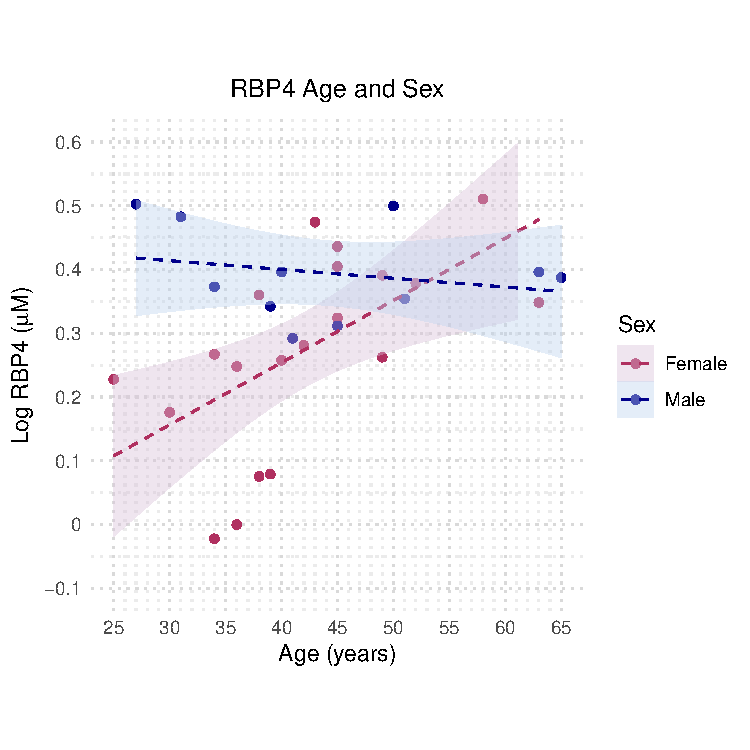
\includegraphics[width=0.5\linewidth]{StatisticalAnalysis_files/figure-latex/plots for RBP4-1}
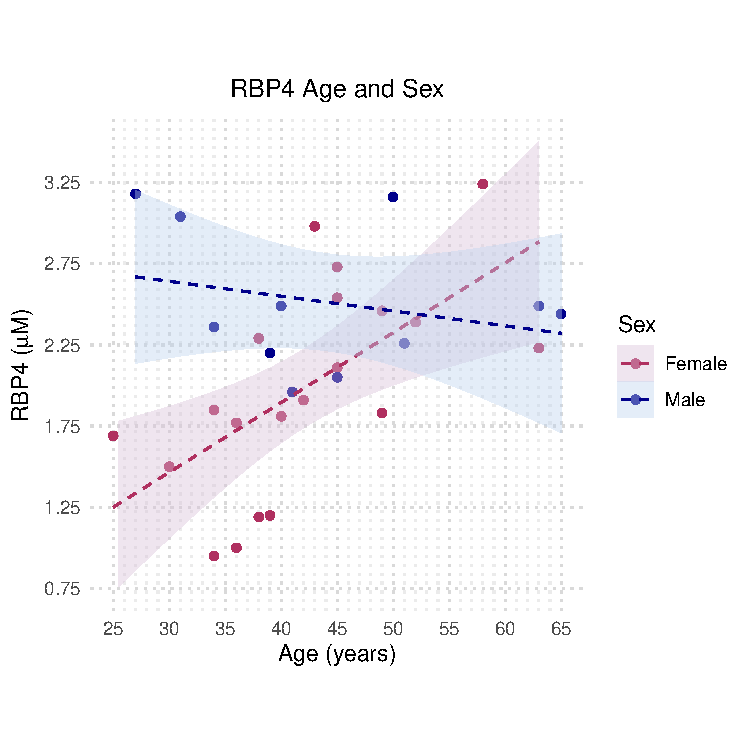
\includegraphics[width=0.5\linewidth]{StatisticalAnalysis_files/figure-latex/plots for RBP4-2}

\newpage

\subsection{Post-hoc analysis of RBP4 and
eGFR}\label{post-hoc-analysis-of-rbp4-and-egfr}

\begin{Shaded}
\begin{Highlighting}[]
\FunctionTok{summary}\NormalTok{(}\FunctionTok{lm}\NormalTok{(LRBP4}\SpecialCharTok{\textasciitilde{}}\NormalTok{eGFR,vao))}
\end{Highlighting}
\end{Shaded}

\begin{verbatim}
## 
## Call:
## lm(formula = LRBP4 ~ eGFR, data = vao)
## 
## Residuals:
##       Min        1Q    Median        3Q       Max 
## -0.277030 -0.051103  0.009991  0.070393  0.232258 
## 
## Coefficients:
##              Estimate Std. Error t value Pr(>|t|)   
## (Intercept)  0.673248   0.222715   3.023  0.00519 **
## eGFR        -0.003267   0.002029  -1.611  0.11810   
## ---
## Signif. codes:  0 '***' 0.001 '**' 0.01 '*' 0.05 '.' 0.1 ' ' 1
## 
## Residual standard error: 0.1364 on 29 degrees of freedom
## Multiple R-squared:  0.0821, Adjusted R-squared:  0.05045 
## F-statistic: 2.594 on 1 and 29 DF,  p-value: 0.1181
\end{verbatim}

\begin{Shaded}
\begin{Highlighting}[]
\FunctionTok{summary}\NormalTok{(}\FunctionTok{lm}\NormalTok{(LRBP4}\SpecialCharTok{\textasciitilde{}}\NormalTok{eGFR}\SpecialCharTok{*}\NormalTok{Sex,vao))}
\end{Highlighting}
\end{Shaded}

\begin{verbatim}
## 
## Call:
## lm(formula = LRBP4 ~ eGFR * Sex, data = vao)
## 
## Residuals:
##      Min       1Q   Median       3Q      Max 
## -0.20730 -0.06922  0.01266  0.07022  0.23966 
## 
## Coefficients:
##               Estimate Std. Error t value Pr(>|t|)    
## (Intercept)   0.832255   0.224461   3.708 0.000954 ***
## eGFR         -0.005153   0.002057  -2.505 0.018573 *  
## SexMale      -0.546204   0.470518  -1.161 0.255861    
## eGFR:SexMale  0.006133   0.004256   1.441 0.161035    
## ---
## Signif. codes:  0 '***' 0.001 '**' 0.01 '*' 0.05 '.' 0.1 ' ' 1
## 
## Residual standard error: 0.1206 on 27 degrees of freedom
## Multiple R-squared:  0.3319, Adjusted R-squared:  0.2576 
## F-statistic: 4.471 on 3 and 27 DF,  p-value: 0.0113
\end{verbatim}

\begin{quote}
eGFR is not a significant correlate for RBP4 (p=0.12) eGFR as an
interaction term with sex is also not significant (p=0.16)
\end{quote}

\newpage

\section{TTR Model}\label{ttr-model}

\begin{Shaded}
\begin{Highlighting}[]
\NormalTok{vao}\SpecialCharTok{$}\NormalTok{LTTR}\OtherTok{\textless{}{-}}\FunctionTok{log10}\NormalTok{(vao}\SpecialCharTok{$}\NormalTok{TTR)}

\CommentTok{\#linear regression with BMI, Sex, Age and HOMA{-}IR}
\NormalTok{Tmodel1}\OtherTok{=}\FunctionTok{lm}\NormalTok{(LTTR}\SpecialCharTok{\textasciitilde{}}\NormalTok{BMI}\SpecialCharTok{+}\NormalTok{Sex}\SpecialCharTok{+}\NormalTok{Age}\SpecialCharTok{+}\NormalTok{LHOMAIR,vao)}
\FunctionTok{summary}\NormalTok{(Tmodel1)}
\end{Highlighting}
\end{Shaded}

\begin{verbatim}
## 
## Call:
## lm(formula = LTTR ~ BMI + Sex + Age + LHOMAIR, data = vao)
## 
## Residuals:
##       Min        1Q    Median        3Q       Max 
## -0.221583 -0.037441  0.002198  0.057781  0.207524 
## 
## Coefficients:
##               Estimate Std. Error t value Pr(>|t|)    
## (Intercept)  1.3295758  0.1437198   9.251 1.04e-09 ***
## BMI         -0.0021577  0.0023340  -0.924   0.3637    
## SexMale      0.0955022  0.0418519   2.282   0.0309 *  
## Age          0.0007957  0.0019475   0.409   0.6862    
## LHOMAIR     -0.0137659  0.0377648  -0.365   0.7184    
## ---
## Signif. codes:  0 '***' 0.001 '**' 0.01 '*' 0.05 '.' 0.1 ' ' 1
## 
## Residual standard error: 0.09806 on 26 degrees of freedom
## Multiple R-squared:  0.3276, Adjusted R-squared:  0.2242 
## F-statistic: 3.167 on 4 and 26 DF,  p-value: 0.0302
\end{verbatim}

\begin{Shaded}
\begin{Highlighting}[]
\FunctionTok{vif}\NormalTok{(Tmodel1)}
\end{Highlighting}
\end{Shaded}

\begin{verbatim}
##      BMI      Sex      Age  LHOMAIR 
## 1.597502 1.292650 1.233974 1.259206
\end{verbatim}

\begin{Shaded}
\begin{Highlighting}[]
\CommentTok{\#remove one variable at a time}
\NormalTok{Tmodel2}\OtherTok{=}\FunctionTok{lm}\NormalTok{(LTTR}\SpecialCharTok{\textasciitilde{}}\NormalTok{BMI}\SpecialCharTok{+}\NormalTok{Sex}\SpecialCharTok{+}\NormalTok{Age,vao) }\CommentTok{\#remove HOMA{-}IR}
\NormalTok{Tmodel3}\OtherTok{=}\FunctionTok{lm}\NormalTok{(LTTR}\SpecialCharTok{\textasciitilde{}}\NormalTok{BMI}\SpecialCharTok{+}\NormalTok{Sex}\SpecialCharTok{+}\NormalTok{LHOMAIR, vao) }\CommentTok{\#remove Age}
\NormalTok{Tmodel4}\OtherTok{=}\FunctionTok{lm}\NormalTok{(LTTR}\SpecialCharTok{\textasciitilde{}}\NormalTok{BMI}\SpecialCharTok{+}\NormalTok{Age}\SpecialCharTok{+}\NormalTok{LHOMAIR, vao) }\CommentTok{\#remove Sex}
\NormalTok{Tmodel5}\OtherTok{=}\FunctionTok{lm}\NormalTok{(LTTR}\SpecialCharTok{\textasciitilde{}}\NormalTok{Sex}\SpecialCharTok{+}\NormalTok{Age}\SpecialCharTok{+}\NormalTok{LHOMAIR, vao) }\CommentTok{\#remove BMI}

\FunctionTok{AIC}\NormalTok{(Tmodel1,Tmodel2,Tmodel3,Tmodel4,Tmodel5) }\CommentTok{\#summary of AIC}
\end{Highlighting}
\end{Shaded}

\begin{longtable}[]{@{}lrr@{}}
\toprule\noalign{}
& df & AIC \\
\midrule\noalign{}
\endhead
\bottomrule\noalign{}
\endlastfoot
Tmodel1 & 6 & -49.45143 \\
Tmodel2 & 5 & -51.29340 \\
Tmodel3 & 5 & -51.25302 \\
Tmodel4 & 5 & -45.79239 \\
Tmodel5 & 5 & -50.44884 \\
\end{longtable}

\begin{Shaded}
\begin{Highlighting}[]
\NormalTok{AICT}\OtherTok{\textless{}{-}}\FunctionTok{AIC}\NormalTok{(Tmodel1,Tmodel2,Tmodel3,Tmodel4,Tmodel5) }\CommentTok{\#summary of AIC}
\NormalTok{AICT\_df}\OtherTok{\textless{}{-}}\FunctionTok{data.frame}\NormalTok{(}
  \AttributeTok{Model=}\FunctionTok{c}\NormalTok{(}\StringTok{"Model 1: Full Model"}\NormalTok{, }\StringTok{"Model 2: No HOMA{-}IR"}\NormalTok{, }\StringTok{"Model 3: No Age"}\NormalTok{, }
          \StringTok{"Model 4: No Sex"}\NormalTok{, }\StringTok{"Model 5: No BMI"}\NormalTok{),}
  \AttributeTok{AIC =} \FunctionTok{round}\NormalTok{(AICT}\SpecialCharTok{$}\NormalTok{AIC,}\DecValTok{3}\NormalTok{), }\AttributeTok{DF =}\NormalTok{ AICT}\SpecialCharTok{$}\NormalTok{df)}

\NormalTok{aicT\_table }\OtherTok{\textless{}{-}}\NormalTok{ AICT\_df }\SpecialCharTok{\%\textgreater{}\%}
  \FunctionTok{flextable}\NormalTok{() }\SpecialCharTok{\%\textgreater{}\%}
  \FunctionTok{set\_header\_labels}\NormalTok{(}\AttributeTok{Model =} \StringTok{"Model Description"}\NormalTok{, }\AttributeTok{AIC =} \StringTok{"AIC Value"}\NormalTok{,}
                    \AttributeTok{DF=}\StringTok{"Degrees of Freedom"}\NormalTok{) }\SpecialCharTok{\%\textgreater{}\%}
  \FunctionTok{add\_header\_lines}\NormalTok{(}\AttributeTok{values =} \StringTok{"AIC Comparison of Models for TTR"}\NormalTok{) }\SpecialCharTok{\%\textgreater{}\%}
  \FunctionTok{align}\NormalTok{(}\AttributeTok{part=}\StringTok{"header"}\NormalTok{, }\AttributeTok{align=}\StringTok{"center"}\NormalTok{ ) }\SpecialCharTok{\%\textgreater{}\%}
  \FunctionTok{add\_footer\_lines}\NormalTok{(}\AttributeTok{values =} \StringTok{"Note: Lower AIC values indicate a better model."}\NormalTok{) }\SpecialCharTok{\%\textgreater{}\%}
  \FunctionTok{fontsize}\NormalTok{(}\AttributeTok{part =} \StringTok{"footer"}\NormalTok{, }\AttributeTok{size =} \DecValTok{8}\NormalTok{) }\SpecialCharTok{\%\textgreater{}\%}
  \FunctionTok{set\_table\_properties}\NormalTok{(}\AttributeTok{layout =} \StringTok{"autofit"}\NormalTok{)}
\NormalTok{aicT\_table}
\end{Highlighting}
\end{Shaded}

\global\setlength{\Oldarrayrulewidth}{\arrayrulewidth}

\global\setlength{\Oldtabcolsep}{\tabcolsep}

\setlength{\tabcolsep}{2pt}

\renewcommand*{\arraystretch}{1.5}



\providecommand{\ascline}[3]{\noalign{\global\arrayrulewidth #1}\arrayrulecolor[HTML]{#2}\cline{#3}}

\begin{longtable}[c]{ccc}



\ascline{1.5pt}{666666}{1-3}

\multicolumn{3}{>{}c}{\textcolor[HTML]{000000}{\fontsize{11}{11}\selectfont{\global\setmainfont{Arial}{AIC\ Comparison\ of\ Models\ for\ TTR}}}} \\

\ascline{1.5pt}{666666}{1-3}



\multicolumn{1}{>{}c}{\textcolor[HTML]{000000}{\fontsize{11}{11}\selectfont{\global\setmainfont{Arial}{Model\ Description}}}} & \multicolumn{1}{>{}c}{\textcolor[HTML]{000000}{\fontsize{11}{11}\selectfont{\global\setmainfont{Arial}{AIC\ Value}}}} & \multicolumn{1}{>{}c}{\textcolor[HTML]{000000}{\fontsize{11}{11}\selectfont{\global\setmainfont{Arial}{Degrees\ of\ Freedom}}}} \\

\ascline{1.5pt}{666666}{1-3}\endfirsthead 

\ascline{1.5pt}{666666}{1-3}

\multicolumn{3}{>{}c}{\textcolor[HTML]{000000}{\fontsize{11}{11}\selectfont{\global\setmainfont{Arial}{AIC\ Comparison\ of\ Models\ for\ TTR}}}} \\

\ascline{1.5pt}{666666}{1-3}



\multicolumn{1}{>{}c}{\textcolor[HTML]{000000}{\fontsize{11}{11}\selectfont{\global\setmainfont{Arial}{Model\ Description}}}} & \multicolumn{1}{>{}c}{\textcolor[HTML]{000000}{\fontsize{11}{11}\selectfont{\global\setmainfont{Arial}{AIC\ Value}}}} & \multicolumn{1}{>{}c}{\textcolor[HTML]{000000}{\fontsize{11}{11}\selectfont{\global\setmainfont{Arial}{Degrees\ of\ Freedom}}}} \\

\ascline{1.5pt}{666666}{1-3}\endhead



\multicolumn{3}{>{}l}{\textcolor[HTML]{000000}{\fontsize{8}{8}\selectfont{\global\setmainfont{Arial}{Note:\ Lower\ AIC\ values\ indicate\ a\ better\ model.}}}} \\

\endlastfoot



\multicolumn{1}{>{}l}{\textcolor[HTML]{000000}{\fontsize{11}{11}\selectfont{\global\setmainfont{Arial}{Model\ 1:\ Full\ Model}}}} & \multicolumn{1}{>{}r}{\textcolor[HTML]{000000}{\fontsize{11}{11}\selectfont{\global\setmainfont{Arial}{-49.451}}}} & \multicolumn{1}{>{}r}{\textcolor[HTML]{000000}{\fontsize{11}{11}\selectfont{\global\setmainfont{Arial}{6}}}} \\





\multicolumn{1}{>{}l}{\textcolor[HTML]{000000}{\fontsize{11}{11}\selectfont{\global\setmainfont{Arial}{Model\ 2:\ No\ HOMA-IR}}}} & \multicolumn{1}{>{}r}{\textcolor[HTML]{000000}{\fontsize{11}{11}\selectfont{\global\setmainfont{Arial}{-51.293}}}} & \multicolumn{1}{>{}r}{\textcolor[HTML]{000000}{\fontsize{11}{11}\selectfont{\global\setmainfont{Arial}{5}}}} \\





\multicolumn{1}{>{}l}{\textcolor[HTML]{000000}{\fontsize{11}{11}\selectfont{\global\setmainfont{Arial}{Model\ 3:\ No\ Age}}}} & \multicolumn{1}{>{}r}{\textcolor[HTML]{000000}{\fontsize{11}{11}\selectfont{\global\setmainfont{Arial}{-51.253}}}} & \multicolumn{1}{>{}r}{\textcolor[HTML]{000000}{\fontsize{11}{11}\selectfont{\global\setmainfont{Arial}{5}}}} \\





\multicolumn{1}{>{}l}{\textcolor[HTML]{000000}{\fontsize{11}{11}\selectfont{\global\setmainfont{Arial}{Model\ 4:\ No\ Sex}}}} & \multicolumn{1}{>{}r}{\textcolor[HTML]{000000}{\fontsize{11}{11}\selectfont{\global\setmainfont{Arial}{-45.792}}}} & \multicolumn{1}{>{}r}{\textcolor[HTML]{000000}{\fontsize{11}{11}\selectfont{\global\setmainfont{Arial}{5}}}} \\





\multicolumn{1}{>{}l}{\textcolor[HTML]{000000}{\fontsize{11}{11}\selectfont{\global\setmainfont{Arial}{Model\ 5:\ No\ BMI}}}} & \multicolumn{1}{>{}r}{\textcolor[HTML]{000000}{\fontsize{11}{11}\selectfont{\global\setmainfont{Arial}{-50.449}}}} & \multicolumn{1}{>{}r}{\textcolor[HTML]{000000}{\fontsize{11}{11}\selectfont{\global\setmainfont{Arial}{5}}}} \\

\ascline{1.5pt}{666666}{1-3}



\end{longtable}



\arrayrulecolor[HTML]{000000}

\global\setlength{\arrayrulewidth}{\Oldarrayrulewidth}

\global\setlength{\tabcolsep}{\Oldtabcolsep}

\renewcommand*{\arraystretch}{1}

\begin{Shaded}
\begin{Highlighting}[]
\DocumentationTok{\#\#remove HOMA{-}IR (lowest AIC)}
\CommentTok{\#add interaction terms for Age and Sex which are not correlated}
\NormalTok{Tmodel6}\OtherTok{=}\FunctionTok{lm}\NormalTok{(LTTR}\SpecialCharTok{\textasciitilde{}}\NormalTok{Sex}\SpecialCharTok{+}\NormalTok{Age}\SpecialCharTok{+}\NormalTok{BMI}\SpecialCharTok{+}\NormalTok{Age}\SpecialCharTok{*}\NormalTok{Sex,vao)}
\FunctionTok{summary}\NormalTok{(Tmodel6)}
\end{Highlighting}
\end{Shaded}

\begin{verbatim}
## 
## Call:
## lm(formula = LTTR ~ Sex + Age + BMI + Age * Sex, data = vao)
## 
## Residuals:
##       Min        1Q    Median        3Q       Max 
## -0.202202 -0.031876 -0.006347  0.048701  0.199926 
## 
## Coefficients:
##              Estimate Std. Error t value Pr(>|t|)    
## (Intercept)  1.150995   0.151538   7.595 4.61e-08 ***
## SexMale      0.421700   0.146241   2.884  0.00779 ** 
## Age          0.004725   0.002363   1.999  0.05613 .  
## BMI         -0.001957   0.002049  -0.955  0.34846    
## SexMale:Age -0.007491   0.003233  -2.317  0.02864 *  
## ---
## Signif. codes:  0 '***' 0.001 '**' 0.01 '*' 0.05 '.' 0.1 ' ' 1
## 
## Residual standard error: 0.08951 on 26 degrees of freedom
## Multiple R-squared:  0.4398, Adjusted R-squared:  0.3537 
## F-statistic: 5.104 on 4 and 26 DF,  p-value: 0.003592
\end{verbatim}

\begin{Shaded}
\begin{Highlighting}[]
\FunctionTok{AIC}\NormalTok{(Tmodel6,Tmodel2)}
\end{Highlighting}
\end{Shaded}

\begin{longtable}[]{@{}lrr@{}}
\toprule\noalign{}
& df & AIC \\
\midrule\noalign{}
\endhead
\bottomrule\noalign{}
\endlastfoot
Tmodel6 & 6 & -55.11268 \\
Tmodel2 & 5 & -51.29340 \\
\end{longtable}

\begin{Shaded}
\begin{Highlighting}[]
\FunctionTok{anova}\NormalTok{(Tmodel6,Tmodel2)}
\end{Highlighting}
\end{Shaded}

\begin{longtable}[]{@{}rrrrrr@{}}
\toprule\noalign{}
Res.Df & RSS & Df & Sum of Sq & F & Pr(\textgreater F) \\
\midrule\noalign{}
\endhead
\bottomrule\noalign{}
\endlastfoot
26 & 0.2082919 & NA & NA & NA & NA \\
27 & 0.2513029 & -1 & -0.043011 & 5.368841 & 0.0286386 \\
\end{longtable}

\begin{Shaded}
\begin{Highlighting}[]
\DocumentationTok{\#\#inclusion of interaction term improves model}
\DocumentationTok{\#\#\#Model now TTR\textasciitilde{}Sex+BMI+Age+Age*Sex}

\CommentTok{\#remove terms}
\NormalTok{Tmodel7}\OtherTok{=}\FunctionTok{lm}\NormalTok{(LTTR}\SpecialCharTok{\textasciitilde{}}\NormalTok{Sex}\SpecialCharTok{+}\NormalTok{Age}\SpecialCharTok{+}\NormalTok{Age}\SpecialCharTok{*}\NormalTok{Sex,vao) }\CommentTok{\# remove BMI}
\NormalTok{Tmodel8}\OtherTok{=}\FunctionTok{lm}\NormalTok{(LTTR}\SpecialCharTok{\textasciitilde{}}\NormalTok{Sex}\SpecialCharTok{+}\NormalTok{BMI,vao) }\CommentTok{\# remove Age}
\NormalTok{Tmodel9}\OtherTok{=}\FunctionTok{lm}\NormalTok{(LTTR}\SpecialCharTok{\textasciitilde{}}\NormalTok{Age}\SpecialCharTok{+}\NormalTok{BMI,vao) }\CommentTok{\#remove Sex}

\NormalTok{AICT\_iterm}\OtherTok{\textless{}{-}}\FunctionTok{AIC}\NormalTok{(Tmodel6,Tmodel7,Tmodel8,Tmodel9) }\CommentTok{\#summary of AIC}
\NormalTok{AICT\_iterm\_df}\OtherTok{\textless{}{-}}\FunctionTok{data.frame}\NormalTok{(}
  \AttributeTok{Model=}\FunctionTok{c}\NormalTok{(}\StringTok{"Full Model: Sex+Age+BMI+AgexSex"}\NormalTok{,}
          \StringTok{"Remove BMI: Sex+Age+AgexSex"}\NormalTok{,}
          \StringTok{"Remove Age: Sex+BMI"}\NormalTok{,}
          \StringTok{"Remove Sex: Age+BMI"}\NormalTok{),}
  \AttributeTok{AIC =} \FunctionTok{round}\NormalTok{(AICT\_iterm}\SpecialCharTok{$}\NormalTok{AIC,}\DecValTok{3}\NormalTok{), }\AttributeTok{DF =}\NormalTok{ AICT\_iterm}\SpecialCharTok{$}\NormalTok{df)}

\NormalTok{aicT\_iterm\_table }\OtherTok{\textless{}{-}}\NormalTok{ AICT\_iterm\_df }\SpecialCharTok{\%\textgreater{}\%}
  \FunctionTok{flextable}\NormalTok{() }\SpecialCharTok{\%\textgreater{}\%}
  \FunctionTok{set\_header\_labels}\NormalTok{(}\AttributeTok{Model =} \StringTok{"Model Description"}\NormalTok{, }\AttributeTok{AIC =} \StringTok{"AIC Value"}\NormalTok{,}
                    \AttributeTok{DF=}\StringTok{"Degrees of Freedom"}\NormalTok{) }\SpecialCharTok{\%\textgreater{}\%}
  \FunctionTok{add\_header\_lines}\NormalTok{(}\AttributeTok{values =} \StringTok{"AIC Comparison of Models for TTR"}\NormalTok{) }\SpecialCharTok{\%\textgreater{}\%}
  \FunctionTok{align}\NormalTok{(}\AttributeTok{part=}\StringTok{"header"}\NormalTok{, }\AttributeTok{align=}\StringTok{"center"}\NormalTok{ ) }\SpecialCharTok{\%\textgreater{}\%}
  \FunctionTok{add\_footer\_lines}\NormalTok{(}\AttributeTok{values =} \StringTok{"Note: Lower AIC values indicate a better model."}\NormalTok{) }\SpecialCharTok{\%\textgreater{}\%}
  \FunctionTok{fontsize}\NormalTok{(}\AttributeTok{part =} \StringTok{"footer"}\NormalTok{, }\AttributeTok{size =} \DecValTok{8}\NormalTok{) }\SpecialCharTok{\%\textgreater{}\%}
  \FunctionTok{set\_table\_properties}\NormalTok{(}\AttributeTok{layout =} \StringTok{"autofit"}\NormalTok{)}
\NormalTok{aicT\_iterm\_table}
\end{Highlighting}
\end{Shaded}

\global\setlength{\Oldarrayrulewidth}{\arrayrulewidth}

\global\setlength{\Oldtabcolsep}{\tabcolsep}

\setlength{\tabcolsep}{2pt}

\renewcommand*{\arraystretch}{1.5}



\providecommand{\ascline}[3]{\noalign{\global\arrayrulewidth #1}\arrayrulecolor[HTML]{#2}\cline{#3}}

\begin{longtable}[c]{ccc}



\ascline{1.5pt}{666666}{1-3}

\multicolumn{3}{>{}c}{\textcolor[HTML]{000000}{\fontsize{11}{11}\selectfont{\global\setmainfont{Arial}{AIC\ Comparison\ of\ Models\ for\ TTR}}}} \\

\ascline{1.5pt}{666666}{1-3}



\multicolumn{1}{>{}c}{\textcolor[HTML]{000000}{\fontsize{11}{11}\selectfont{\global\setmainfont{Arial}{Model\ Description}}}} & \multicolumn{1}{>{}c}{\textcolor[HTML]{000000}{\fontsize{11}{11}\selectfont{\global\setmainfont{Arial}{AIC\ Value}}}} & \multicolumn{1}{>{}c}{\textcolor[HTML]{000000}{\fontsize{11}{11}\selectfont{\global\setmainfont{Arial}{Degrees\ of\ Freedom}}}} \\

\ascline{1.5pt}{666666}{1-3}\endfirsthead 

\ascline{1.5pt}{666666}{1-3}

\multicolumn{3}{>{}c}{\textcolor[HTML]{000000}{\fontsize{11}{11}\selectfont{\global\setmainfont{Arial}{AIC\ Comparison\ of\ Models\ for\ TTR}}}} \\

\ascline{1.5pt}{666666}{1-3}



\multicolumn{1}{>{}c}{\textcolor[HTML]{000000}{\fontsize{11}{11}\selectfont{\global\setmainfont{Arial}{Model\ Description}}}} & \multicolumn{1}{>{}c}{\textcolor[HTML]{000000}{\fontsize{11}{11}\selectfont{\global\setmainfont{Arial}{AIC\ Value}}}} & \multicolumn{1}{>{}c}{\textcolor[HTML]{000000}{\fontsize{11}{11}\selectfont{\global\setmainfont{Arial}{Degrees\ of\ Freedom}}}} \\

\ascline{1.5pt}{666666}{1-3}\endhead



\multicolumn{3}{>{}l}{\textcolor[HTML]{000000}{\fontsize{8}{8}\selectfont{\global\setmainfont{Arial}{Note:\ Lower\ AIC\ values\ indicate\ a\ better\ model.}}}} \\

\endlastfoot



\multicolumn{1}{>{}l}{\textcolor[HTML]{000000}{\fontsize{11}{11}\selectfont{\global\setmainfont{Arial}{Full\ Model:\ Sex+Age+BMI+AgexSex}}}} & \multicolumn{1}{>{}r}{\textcolor[HTML]{000000}{\fontsize{11}{11}\selectfont{\global\setmainfont{Arial}{-55.113}}}} & \multicolumn{1}{>{}r}{\textcolor[HTML]{000000}{\fontsize{11}{11}\selectfont{\global\setmainfont{Arial}{6}}}} \\





\multicolumn{1}{>{}l}{\textcolor[HTML]{000000}{\fontsize{11}{11}\selectfont{\global\setmainfont{Arial}{Remove\ BMI:\ Sex+Age+AgexSex}}}} & \multicolumn{1}{>{}r}{\textcolor[HTML]{000000}{\fontsize{11}{11}\selectfont{\global\setmainfont{Arial}{-56.044}}}} & \multicolumn{1}{>{}r}{\textcolor[HTML]{000000}{\fontsize{11}{11}\selectfont{\global\setmainfont{Arial}{5}}}} \\





\multicolumn{1}{>{}l}{\textcolor[HTML]{000000}{\fontsize{11}{11}\selectfont{\global\setmainfont{Arial}{Remove\ Age:\ Sex+BMI}}}} & \multicolumn{1}{>{}r}{\textcolor[HTML]{000000}{\fontsize{11}{11}\selectfont{\global\setmainfont{Arial}{-52.979}}}} & \multicolumn{1}{>{}r}{\textcolor[HTML]{000000}{\fontsize{11}{11}\selectfont{\global\setmainfont{Arial}{4}}}} \\





\multicolumn{1}{>{}l}{\textcolor[HTML]{000000}{\fontsize{11}{11}\selectfont{\global\setmainfont{Arial}{Remove\ Sex:\ Age+BMI}}}} & \multicolumn{1}{>{}r}{\textcolor[HTML]{000000}{\fontsize{11}{11}\selectfont{\global\setmainfont{Arial}{-47.742}}}} & \multicolumn{1}{>{}r}{\textcolor[HTML]{000000}{\fontsize{11}{11}\selectfont{\global\setmainfont{Arial}{4}}}} \\

\ascline{1.5pt}{666666}{1-3}



\end{longtable}



\arrayrulecolor[HTML]{000000}

\global\setlength{\arrayrulewidth}{\Oldarrayrulewidth}

\global\setlength{\tabcolsep}{\Oldtabcolsep}

\renewcommand*{\arraystretch}{1}

\begin{Shaded}
\begin{Highlighting}[]
\CommentTok{\#lowest AIC removing BMI}
\CommentTok{\#confirm with anova}
\FunctionTok{anova}\NormalTok{(Tmodel7,Tmodel8)}
\end{Highlighting}
\end{Shaded}

\begin{longtable}[]{@{}rrrrrr@{}}
\toprule\noalign{}
Res.Df & RSS & Df & Sum of Sq & F & Pr(\textgreater F) \\
\midrule\noalign{}
\endhead
\bottomrule\noalign{}
\endlastfoot
27 & 0.2155956 & NA & NA & NA & NA \\
28 & 0.2538616 & -1 & -0.038266 & 4.792217 & 0.0374116 \\
\end{longtable}

\begin{Shaded}
\begin{Highlighting}[]
\FunctionTok{anova}\NormalTok{(Tmodel6,Tmodel7) }\CommentTok{\# removing BMI leads to lower AIC, stat. sig.}
\end{Highlighting}
\end{Shaded}

\begin{longtable}[]{@{}rrrrrr@{}}
\toprule\noalign{}
Res.Df & RSS & Df & Sum of Sq & F & Pr(\textgreater F) \\
\midrule\noalign{}
\endhead
\bottomrule\noalign{}
\endlastfoot
26 & 0.2082919 & NA & NA & NA & NA \\
27 & 0.2155956 & -1 & -0.0073038 & 0.911693 & 0.3484596 \\
\end{longtable}

\begin{Shaded}
\begin{Highlighting}[]
\DocumentationTok{\#\#\#Model now TTR \textasciitilde{} Sex + Age + Age * Sex}

\CommentTok{\#does adding HOMA{-}IR back into the model improve the model?}
\NormalTok{Tmodel10}\OtherTok{=}\FunctionTok{lm}\NormalTok{(LTTR}\SpecialCharTok{\textasciitilde{}}\NormalTok{Sex}\SpecialCharTok{+}\NormalTok{Age}\SpecialCharTok{+}\NormalTok{Age}\SpecialCharTok{*}\NormalTok{Sex}\SpecialCharTok{+}\NormalTok{LHOMAIR,vao)}
\FunctionTok{summary}\NormalTok{(Tmodel10)}
\end{Highlighting}
\end{Shaded}

\begin{verbatim}
## 
## Call:
## lm(formula = LTTR ~ Sex + Age + Age * Sex + LHOMAIR, data = vao)
## 
## Residuals:
##       Min        1Q    Median        3Q       Max 
## -0.219463 -0.034099 -0.000104  0.048686  0.205280 
## 
## Coefficients:
##              Estimate Std. Error t value Pr(>|t|)    
## (Intercept)  1.060046   0.107323   9.877 2.74e-10 ***
## SexMale      0.442935   0.145917   3.036   0.0054 ** 
## Age          0.005092   0.002397   2.124   0.0433 *  
## LHOMAIR     -0.015603   0.033632  -0.464   0.6465    
## SexMale:Age -0.007621   0.003279  -2.324   0.0282 *  
## ---
## Signif. codes:  0 '***' 0.001 '**' 0.01 '*' 0.05 '.' 0.1 ' ' 1
## 
## Residual standard error: 0.09069 on 26 degrees of freedom
## Multiple R-squared:  0.425,  Adjusted R-squared:  0.3365 
## F-statistic: 4.803 on 4 and 26 DF,  p-value: 0.004906
\end{verbatim}

\begin{Shaded}
\begin{Highlighting}[]
\FunctionTok{AIC}\NormalTok{(Tmodel7, Tmodel10)}
\end{Highlighting}
\end{Shaded}

\begin{longtable}[]{@{}lrr@{}}
\toprule\noalign{}
& df & AIC \\
\midrule\noalign{}
\endhead
\bottomrule\noalign{}
\endlastfoot
Tmodel7 & 5 & -56.04428 \\
Tmodel10 & 6 & -54.29986 \\
\end{longtable}

\begin{Shaded}
\begin{Highlighting}[]
\FunctionTok{anova}\NormalTok{(Tmodel7, Tmodel10) }\CommentTok{\#no, both from ANOVA and AIC, HOMA does not improve the model}
\end{Highlighting}
\end{Shaded}

\begin{longtable}[]{@{}rrrrrr@{}}
\toprule\noalign{}
Res.Df & RSS & Df & Sum of Sq & F & Pr(\textgreater F) \\
\midrule\noalign{}
\endhead
\bottomrule\noalign{}
\endlastfoot
27 & 0.2155956 & NA & NA & NA & NA \\
26 & 0.2138255 & 1 & 0.0017702 & 0.2152428 & 0.6465498 \\
\end{longtable}

\begin{Shaded}
\begin{Highlighting}[]
\CommentTok{\#does the interaction term improve the model?}
\NormalTok{Tmodel11}\OtherTok{=}\FunctionTok{lm}\NormalTok{(LTTR}\SpecialCharTok{\textasciitilde{}}\NormalTok{Sex}\SpecialCharTok{+}\NormalTok{Age,vao)}
\FunctionTok{AIC}\NormalTok{(Tmodel7,Tmodel11)}
\end{Highlighting}
\end{Shaded}

\begin{longtable}[]{@{}lrr@{}}
\toprule\noalign{}
& df & AIC \\
\midrule\noalign{}
\endhead
\bottomrule\noalign{}
\endlastfoot
Tmodel7 & 5 & -56.04428 \\
Tmodel11 & 4 & -51.95223 \\
\end{longtable}

\begin{Shaded}
\begin{Highlighting}[]
\FunctionTok{anova}\NormalTok{(Tmodel7,Tmodel11) }\CommentTok{\#yes}
\end{Highlighting}
\end{Shaded}

\begin{longtable}[]{@{}rrrrrr@{}}
\toprule\noalign{}
Res.Df & RSS & Df & Sum of Sq & F & Pr(\textgreater F) \\
\midrule\noalign{}
\endhead
\bottomrule\noalign{}
\endlastfoot
27 & 0.2155956 & NA & NA & NA & NA \\
28 & 0.2624138 & -1 & -0.0468181 & 5.863243 & 0.022454 \\
\end{longtable}

\begin{Shaded}
\begin{Highlighting}[]
\CommentTok{\#is this the simplest model?}
\NormalTok{Tmodel12}\OtherTok{=}\FunctionTok{lm}\NormalTok{(LTTR}\SpecialCharTok{\textasciitilde{}}\NormalTok{Sex,vao) }\CommentTok{\#Sex alone}
\NormalTok{Tmodel13}\OtherTok{=}\FunctionTok{lm}\NormalTok{(LTTR}\SpecialCharTok{\textasciitilde{}}\NormalTok{Age,vao) }\CommentTok{\#Age alone}


\NormalTok{AICT2}\OtherTok{\textless{}{-}}\FunctionTok{AIC}\NormalTok{(Tmodel7,Tmodel11,Tmodel12,Tmodel13) }\CommentTok{\#summary of AIC}
\NormalTok{AICT2\_df}\OtherTok{\textless{}{-}}\FunctionTok{data.frame}\NormalTok{(}
  \AttributeTok{Model=}\FunctionTok{c}\NormalTok{(}\StringTok{"Sex + Age + Sex x Age"}\NormalTok{,}
          \StringTok{"Sex + Age"}\NormalTok{,}\StringTok{"Sex"}\NormalTok{, }\StringTok{"Age"}\NormalTok{),}
  \AttributeTok{AIC =} \FunctionTok{round}\NormalTok{(AICT2}\SpecialCharTok{$}\NormalTok{AIC,}\DecValTok{3}\NormalTok{), }\AttributeTok{DF =}\NormalTok{ AICT2}\SpecialCharTok{$}\NormalTok{df)}

\NormalTok{aicT2\_table }\OtherTok{\textless{}{-}}\NormalTok{ AICT2\_df }\SpecialCharTok{\%\textgreater{}\%}
  \FunctionTok{flextable}\NormalTok{() }\SpecialCharTok{\%\textgreater{}\%}
  \FunctionTok{set\_header\_labels}\NormalTok{(}\AttributeTok{Model =} \StringTok{"Model Description"}\NormalTok{, }\AttributeTok{AIC =} \StringTok{"AIC Value"}\NormalTok{,}
                    \AttributeTok{DF=}\StringTok{"Degrees of Freedom"}\NormalTok{) }\SpecialCharTok{\%\textgreater{}\%}
  \FunctionTok{add\_header\_lines}\NormalTok{(}\AttributeTok{values =} \StringTok{"AIC Comparison of Models for TTR"}\NormalTok{) }\SpecialCharTok{\%\textgreater{}\%}
  \FunctionTok{align}\NormalTok{(}\AttributeTok{part=}\StringTok{"header"}\NormalTok{, }\AttributeTok{align=}\StringTok{"center"}\NormalTok{ ) }\SpecialCharTok{\%\textgreater{}\%}
  \FunctionTok{add\_footer\_lines}\NormalTok{(}\AttributeTok{values=}\StringTok{"Note: Lower AIC values indicate a better model."}\NormalTok{) }\SpecialCharTok{\%\textgreater{}\%}
  \FunctionTok{fontsize}\NormalTok{(}\AttributeTok{part =} \StringTok{"footer"}\NormalTok{, }\AttributeTok{size =} \DecValTok{8}\NormalTok{) }\SpecialCharTok{\%\textgreater{}\%}
  \FunctionTok{set\_table\_properties}\NormalTok{(}\AttributeTok{layout =} \StringTok{"autofit"}\NormalTok{)}
\NormalTok{aicT2\_table}
\end{Highlighting}
\end{Shaded}

\global\setlength{\Oldarrayrulewidth}{\arrayrulewidth}

\global\setlength{\Oldtabcolsep}{\tabcolsep}

\setlength{\tabcolsep}{2pt}

\renewcommand*{\arraystretch}{1.5}



\providecommand{\ascline}[3]{\noalign{\global\arrayrulewidth #1}\arrayrulecolor[HTML]{#2}\cline{#3}}

\begin{longtable}[c]{ccc}



\ascline{1.5pt}{666666}{1-3}

\multicolumn{3}{>{}c}{\textcolor[HTML]{000000}{\fontsize{11}{11}\selectfont{\global\setmainfont{Arial}{AIC\ Comparison\ of\ Models\ for\ TTR}}}} \\

\ascline{1.5pt}{666666}{1-3}



\multicolumn{1}{>{}c}{\textcolor[HTML]{000000}{\fontsize{11}{11}\selectfont{\global\setmainfont{Arial}{Model\ Description}}}} & \multicolumn{1}{>{}c}{\textcolor[HTML]{000000}{\fontsize{11}{11}\selectfont{\global\setmainfont{Arial}{AIC\ Value}}}} & \multicolumn{1}{>{}c}{\textcolor[HTML]{000000}{\fontsize{11}{11}\selectfont{\global\setmainfont{Arial}{Degrees\ of\ Freedom}}}} \\

\ascline{1.5pt}{666666}{1-3}\endfirsthead 

\ascline{1.5pt}{666666}{1-3}

\multicolumn{3}{>{}c}{\textcolor[HTML]{000000}{\fontsize{11}{11}\selectfont{\global\setmainfont{Arial}{AIC\ Comparison\ of\ Models\ for\ TTR}}}} \\

\ascline{1.5pt}{666666}{1-3}



\multicolumn{1}{>{}c}{\textcolor[HTML]{000000}{\fontsize{11}{11}\selectfont{\global\setmainfont{Arial}{Model\ Description}}}} & \multicolumn{1}{>{}c}{\textcolor[HTML]{000000}{\fontsize{11}{11}\selectfont{\global\setmainfont{Arial}{AIC\ Value}}}} & \multicolumn{1}{>{}c}{\textcolor[HTML]{000000}{\fontsize{11}{11}\selectfont{\global\setmainfont{Arial}{Degrees\ of\ Freedom}}}} \\

\ascline{1.5pt}{666666}{1-3}\endhead



\multicolumn{3}{>{}l}{\textcolor[HTML]{000000}{\fontsize{8}{8}\selectfont{\global\setmainfont{Arial}{Note:\ Lower\ AIC\ values\ indicate\ a\ better\ model.}}}} \\

\endlastfoot



\multicolumn{1}{>{}l}{\textcolor[HTML]{000000}{\fontsize{11}{11}\selectfont{\global\setmainfont{Arial}{Sex\ +\ Age\ +\ Sex\ x\ Age}}}} & \multicolumn{1}{>{}r}{\textcolor[HTML]{000000}{\fontsize{11}{11}\selectfont{\global\setmainfont{Arial}{-56.044}}}} & \multicolumn{1}{>{}r}{\textcolor[HTML]{000000}{\fontsize{11}{11}\selectfont{\global\setmainfont{Arial}{5}}}} \\





\multicolumn{1}{>{}l}{\textcolor[HTML]{000000}{\fontsize{11}{11}\selectfont{\global\setmainfont{Arial}{Sex\ +\ Age}}}} & \multicolumn{1}{>{}r}{\textcolor[HTML]{000000}{\fontsize{11}{11}\selectfont{\global\setmainfont{Arial}{-51.952}}}} & \multicolumn{1}{>{}r}{\textcolor[HTML]{000000}{\fontsize{11}{11}\selectfont{\global\setmainfont{Arial}{4}}}} \\





\multicolumn{1}{>{}l}{\textcolor[HTML]{000000}{\fontsize{11}{11}\selectfont{\global\setmainfont{Arial}{Sex}}}} & \multicolumn{1}{>{}r}{\textcolor[HTML]{000000}{\fontsize{11}{11}\selectfont{\global\setmainfont{Arial}{-52.919}}}} & \multicolumn{1}{>{}r}{\textcolor[HTML]{000000}{\fontsize{11}{11}\selectfont{\global\setmainfont{Arial}{3}}}} \\





\multicolumn{1}{>{}l}{\textcolor[HTML]{000000}{\fontsize{11}{11}\selectfont{\global\setmainfont{Arial}{Age}}}} & \multicolumn{1}{>{}r}{\textcolor[HTML]{000000}{\fontsize{11}{11}\selectfont{\global\setmainfont{Arial}{-44.500}}}} & \multicolumn{1}{>{}r}{\textcolor[HTML]{000000}{\fontsize{11}{11}\selectfont{\global\setmainfont{Arial}{3}}}} \\

\ascline{1.5pt}{666666}{1-3}



\end{longtable}



\arrayrulecolor[HTML]{000000}

\global\setlength{\arrayrulewidth}{\Oldarrayrulewidth}

\global\setlength{\tabcolsep}{\Oldtabcolsep}

\renewcommand*{\arraystretch}{1}

\begin{Shaded}
\begin{Highlighting}[]
 \CommentTok{\#summary of anova results}
\NormalTok{  p\_values}\OtherTok{\textless{}{-}}\FunctionTok{data.frame}\NormalTok{(}
    \AttributeTok{Comparison=}\FunctionTok{c}\NormalTok{(}\StringTok{"Age+Sex+AgexSex v Age+Sex"}\NormalTok{, }\StringTok{"Age+Sex+AgexSex v Age"}\NormalTok{, }
                 \StringTok{"Age+Sex+AgexSex v Sex"}\NormalTok{),}
    \AttributeTok{P\_value=}\FunctionTok{c}\NormalTok{(}\FunctionTok{round}\NormalTok{(}\FunctionTok{anova}\NormalTok{(Tmodel7,Tmodel11)}\SpecialCharTok{$}\StringTok{"Pr(\textgreater{}F)"}\NormalTok{[}\DecValTok{2}\NormalTok{],}\DecValTok{3}\NormalTok{),}
              \FunctionTok{round}\NormalTok{(}\FunctionTok{anova}\NormalTok{(Tmodel7,Tmodel12)}\SpecialCharTok{$}\StringTok{"Pr(\textgreater{}F)"}\NormalTok{[}\DecValTok{2}\NormalTok{],}\DecValTok{3}\NormalTok{),}
              \FunctionTok{round}\NormalTok{(}\FunctionTok{anova}\NormalTok{(Tmodel7,Tmodel13)}\SpecialCharTok{$}\StringTok{"Pr(\textgreater{}F)"}\NormalTok{[}\DecValTok{2}\NormalTok{],}\DecValTok{3}\NormalTok{)))}
  
\NormalTok{  p\_values }\SpecialCharTok{\%\textgreater{}\%} \FunctionTok{flextable}\NormalTok{() }\SpecialCharTok{\%\textgreater{}\%}
      \FunctionTok{set\_header\_labels}\NormalTok{(}\AttributeTok{Comparison=}\StringTok{"Models"}\NormalTok{, }\AttributeTok{P\_value=}\StringTok{"P{-}value: Probability \textgreater{}F"}\NormalTok{) }\SpecialCharTok{\%\textgreater{}\%}
      \FunctionTok{add\_header\_lines}\NormalTok{(}\AttributeTok{values=}\StringTok{"Is this the simplest model that fits the data best?"}\NormalTok{) }\SpecialCharTok{\%\textgreater{}\%}
      \FunctionTok{align}\NormalTok{(}\AttributeTok{part=}\StringTok{"header"}\NormalTok{, }\AttributeTok{align=}\StringTok{"center"}\NormalTok{ ) }\SpecialCharTok{\%\textgreater{}\%}
      \FunctionTok{set\_table\_properties}\NormalTok{(}\AttributeTok{layout =} \StringTok{"autofit"}\NormalTok{) }\SpecialCharTok{\%\textgreater{}\%}
      \FunctionTok{add\_footer\_lines}\NormalTok{(}\AttributeTok{values =} \StringTok{"Note: p\textless{}0.05 cut{-}off for retaining more complex model"}\NormalTok{) }\SpecialCharTok{\%\textgreater{}\%}
      \FunctionTok{fontsize}\NormalTok{(}\AttributeTok{part =} \StringTok{"footer"}\NormalTok{, }\AttributeTok{size =} \DecValTok{8}\NormalTok{) }
\end{Highlighting}
\end{Shaded}

\global\setlength{\Oldarrayrulewidth}{\arrayrulewidth}

\global\setlength{\Oldtabcolsep}{\tabcolsep}

\setlength{\tabcolsep}{2pt}

\renewcommand*{\arraystretch}{1.5}



\providecommand{\ascline}[3]{\noalign{\global\arrayrulewidth #1}\arrayrulecolor[HTML]{#2}\cline{#3}}

\begin{longtable}[c]{cc}



\ascline{1.5pt}{666666}{1-2}

\multicolumn{2}{>{}c}{\textcolor[HTML]{000000}{\fontsize{11}{11}\selectfont{\global\setmainfont{Arial}{Is\ this\ the\ simplest\ model\ that\ fits\ the\ data\ best?}}}} \\

\ascline{1.5pt}{666666}{1-2}



\multicolumn{1}{>{}c}{\textcolor[HTML]{000000}{\fontsize{11}{11}\selectfont{\global\setmainfont{Arial}{Models}}}} & \multicolumn{1}{>{}c}{\textcolor[HTML]{000000}{\fontsize{11}{11}\selectfont{\global\setmainfont{Arial}{P-value:\ Probability\ >F}}}} \\

\ascline{1.5pt}{666666}{1-2}\endfirsthead 

\ascline{1.5pt}{666666}{1-2}

\multicolumn{2}{>{}c}{\textcolor[HTML]{000000}{\fontsize{11}{11}\selectfont{\global\setmainfont{Arial}{Is\ this\ the\ simplest\ model\ that\ fits\ the\ data\ best?}}}} \\

\ascline{1.5pt}{666666}{1-2}



\multicolumn{1}{>{}c}{\textcolor[HTML]{000000}{\fontsize{11}{11}\selectfont{\global\setmainfont{Arial}{Models}}}} & \multicolumn{1}{>{}c}{\textcolor[HTML]{000000}{\fontsize{11}{11}\selectfont{\global\setmainfont{Arial}{P-value:\ Probability\ >F}}}} \\

\ascline{1.5pt}{666666}{1-2}\endhead



\multicolumn{2}{>{}l}{\textcolor[HTML]{000000}{\fontsize{8}{8}\selectfont{\global\setmainfont{Arial}{Note:\ p<0.05\ cut-off\ for\ retaining\ more\ complex\ model}}}} \\

\endlastfoot



\multicolumn{1}{>{}l}{\textcolor[HTML]{000000}{\fontsize{11}{11}\selectfont{\global\setmainfont{Arial}{Age+Sex+AgexSex\ v\ Age+Sex}}}} & \multicolumn{1}{>{}r}{\textcolor[HTML]{000000}{\fontsize{11}{11}\selectfont{\global\setmainfont{Arial}{0.022}}}} \\





\multicolumn{1}{>{}l}{\textcolor[HTML]{000000}{\fontsize{11}{11}\selectfont{\global\setmainfont{Arial}{Age+Sex+AgexSex\ v\ Age}}}} & \multicolumn{1}{>{}r}{\textcolor[HTML]{000000}{\fontsize{11}{11}\selectfont{\global\setmainfont{Arial}{0.045}}}} \\





\multicolumn{1}{>{}l}{\textcolor[HTML]{000000}{\fontsize{11}{11}\selectfont{\global\setmainfont{Arial}{Age+Sex+AgexSex\ v\ Sex}}}} & \multicolumn{1}{>{}r}{\textcolor[HTML]{000000}{\fontsize{11}{11}\selectfont{\global\setmainfont{Arial}{0.001}}}} \\

\ascline{1.5pt}{666666}{1-2}



\end{longtable}



\arrayrulecolor[HTML]{000000}

\global\setlength{\arrayrulewidth}{\Oldarrayrulewidth}

\global\setlength{\tabcolsep}{\Oldtabcolsep}

\renewcommand*{\arraystretch}{1}

\begin{Shaded}
\begin{Highlighting}[]
  \DocumentationTok{\#\#final model for TTR}
\FunctionTok{summary}\NormalTok{(Tmodel7)}
\end{Highlighting}
\end{Shaded}

\begin{verbatim}
## 
## Call:
## lm(formula = LTTR ~ Sex + Age + Age * Sex, data = vao)
## 
## Residuals:
##       Min        1Q    Median        3Q       Max 
## -0.219703 -0.039820  0.003317  0.047080  0.200418 
## 
## Coefficients:
##              Estimate Std. Error t value Pr(>|t|)    
## (Intercept)  1.039175   0.096013  10.823 2.53e-11 ***
## SexMale      0.451183   0.142710   3.162  0.00385 ** 
## Age          0.005453   0.002233   2.442  0.02145 *  
## SexMale:Age -0.007781   0.003213  -2.421  0.02245 *  
## ---
## Signif. codes:  0 '***' 0.001 '**' 0.01 '*' 0.05 '.' 0.1 ' ' 1
## 
## Residual standard error: 0.08936 on 27 degrees of freedom
## Multiple R-squared:  0.4202, Adjusted R-squared:  0.3558 
## F-statistic: 6.522 on 3 and 27 DF,  p-value: 0.00184
\end{verbatim}

\begin{Shaded}
\begin{Highlighting}[]
\CommentTok{\#variance inflation factors }
\FunctionTok{vif}\NormalTok{(Tmodel7,}\AttributeTok{type=}\FunctionTok{c}\NormalTok{(}\StringTok{"predictor"}\NormalTok{)) }\CommentTok{\#because this model has interaction terms we need to use the GVIF}
\end{Highlighting}
\end{Shaded}

\begin{longtable}[]{@{}lrrrll@{}}
\toprule\noalign{}
& GVIF & Df & GVIF\^{}(1/(2*Df)) & Interacts With & Other Predictors \\
\midrule\noalign{}
\endhead
\bottomrule\noalign{}
\endlastfoot
Sex & 1 & 3 & 1 & Age & -- \\
Age & 1 & 3 & 1 & Sex & -- \\
\end{longtable}

\subsection{TTR Final Model}\label{ttr-final-model}

\begin{quote}
TTR Final Model: TTR \textasciitilde{} Age + Sex + Age x Sex (p=0.02)
\end{quote}

\subsection{TTR Model Plots}\label{ttr-model-plots}

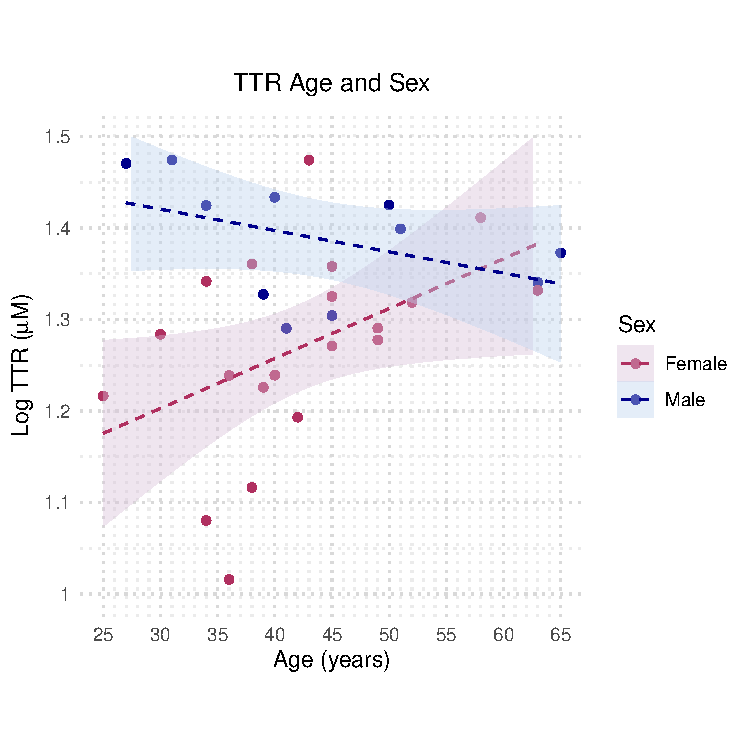
\includegraphics[width=0.5\linewidth]{StatisticalAnalysis_files/figure-latex/TTR plots-1}
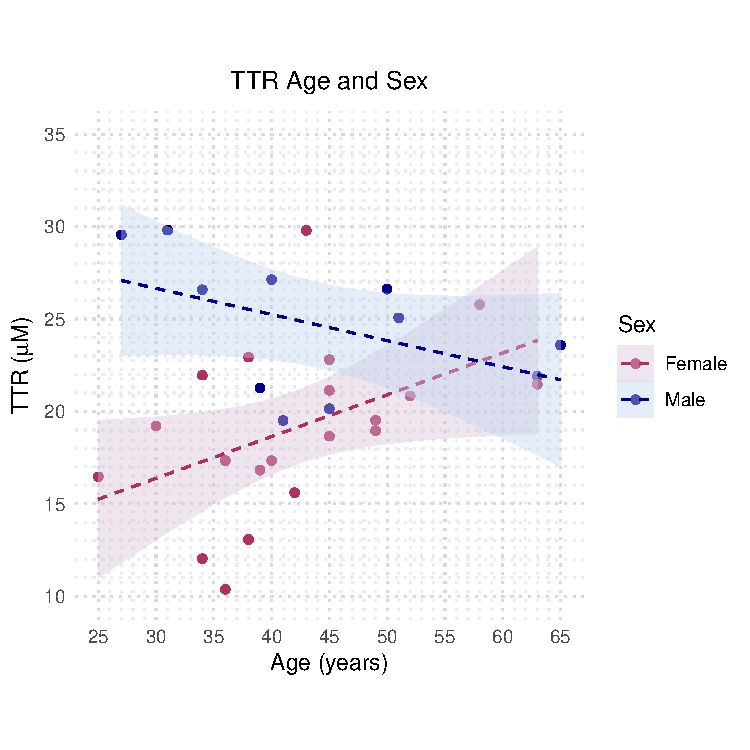
\includegraphics[width=0.5\linewidth]{StatisticalAnalysis_files/figure-latex/TTR plots-2}

\newpage

\section{Retinol Model}\label{retinol-model}

\begin{Shaded}
\begin{Highlighting}[]
\NormalTok{vao}\SpecialCharTok{$}\NormalTok{LROL}\OtherTok{\textless{}{-}}\FunctionTok{log10}\NormalTok{(vao}\SpecialCharTok{$}\NormalTok{Sretinol)}

\CommentTok{\#linear regression with BMI, Sex, Age and HOMAIR}
\NormalTok{Rmodel1}\OtherTok{=}\FunctionTok{lm}\NormalTok{(LROL}\SpecialCharTok{\textasciitilde{}}\NormalTok{BMI}\SpecialCharTok{+}\NormalTok{Sex}\SpecialCharTok{+}\NormalTok{Age}\SpecialCharTok{+}\NormalTok{LHOMAIR,vao)}
\FunctionTok{vif}\NormalTok{(Rmodel1)}
\end{Highlighting}
\end{Shaded}

\begin{verbatim}
##      BMI      Sex      Age  LHOMAIR 
## 1.597502 1.292650 1.233974 1.259206
\end{verbatim}

\begin{Shaded}
\begin{Highlighting}[]
\CommentTok{\#remove one variable at a time}
\NormalTok{Rmodel2}\OtherTok{=}\FunctionTok{lm}\NormalTok{(LROL}\SpecialCharTok{\textasciitilde{}}\NormalTok{BMI}\SpecialCharTok{+}\NormalTok{Sex}\SpecialCharTok{+}\NormalTok{Age,vao) }\CommentTok{\#remove HOMA{-}IR}
\NormalTok{Rmodel3}\OtherTok{=}\FunctionTok{lm}\NormalTok{(LROL}\SpecialCharTok{\textasciitilde{}}\NormalTok{BMI}\SpecialCharTok{+}\NormalTok{Sex}\SpecialCharTok{+}\NormalTok{LHOMAIR, vao) }\CommentTok{\#remove Age}
\NormalTok{Rmodel4}\OtherTok{=}\FunctionTok{lm}\NormalTok{(LROL}\SpecialCharTok{\textasciitilde{}}\NormalTok{BMI}\SpecialCharTok{+}\NormalTok{Age}\SpecialCharTok{+}\NormalTok{LHOMAIR, vao) }\CommentTok{\#remove Sex}
\NormalTok{Rmodel5}\OtherTok{=}\FunctionTok{lm}\NormalTok{(LROL}\SpecialCharTok{\textasciitilde{}}\NormalTok{Sex}\SpecialCharTok{+}\NormalTok{Age}\SpecialCharTok{+}\NormalTok{LHOMAIR, vao) }\CommentTok{\#remove BMI}

\FunctionTok{AIC}\NormalTok{(Rmodel1,Rmodel2,Rmodel3,Rmodel4,Rmodel5) }\CommentTok{\#summary of AIC}
\end{Highlighting}
\end{Shaded}

\begin{longtable}[]{@{}lrr@{}}
\toprule\noalign{}
& df & AIC \\
\midrule\noalign{}
\endhead
\bottomrule\noalign{}
\endlastfoot
Rmodel1 & 6 & -37.11641 \\
Rmodel2 & 5 & -38.95172 \\
Rmodel3 & 5 & -37.12858 \\
Rmodel4 & 5 & -37.23750 \\
Rmodel5 & 5 & -38.03374 \\
\end{longtable}

\begin{Shaded}
\begin{Highlighting}[]
\NormalTok{AICR}\OtherTok{\textless{}{-}}\FunctionTok{AIC}\NormalTok{(Rmodel1,Rmodel2,Rmodel3,Rmodel4,Rmodel5) }\CommentTok{\#summary of AIC}
\NormalTok{AICR\_df}\OtherTok{\textless{}{-}}\FunctionTok{data.frame}\NormalTok{(}
  \AttributeTok{Model=}\FunctionTok{c}\NormalTok{(}\StringTok{"Model 1: Full Model"}\NormalTok{, }\StringTok{"Model 2: No HOMA{-}IR"}\NormalTok{, }\StringTok{"Model 3: No Age"}\NormalTok{,}
          \StringTok{"Model 4: No Sex"}\NormalTok{, }\StringTok{"Model 5: No BMI"}\NormalTok{),}
  \AttributeTok{AIC =}\NormalTok{ AICR}\SpecialCharTok{$}\NormalTok{AIC,}
  \AttributeTok{DF =}\NormalTok{ AICR}\SpecialCharTok{$}\NormalTok{df)}
\NormalTok{aicR\_table }\OtherTok{\textless{}{-}}\NormalTok{ AICR\_df }\SpecialCharTok{\%\textgreater{}\%}
  \FunctionTok{flextable}\NormalTok{() }\SpecialCharTok{\%\textgreater{}\%}
  \FunctionTok{set\_header\_labels}\NormalTok{(}\AttributeTok{Model =} \StringTok{"Model Description"}\NormalTok{, }\AttributeTok{AIC =} \StringTok{"AIC Value"}\NormalTok{,}
                    \AttributeTok{DF=}\StringTok{"Degrees of Freedom"}\NormalTok{) }\SpecialCharTok{\%\textgreater{}\%}
  \FunctionTok{add\_header\_lines}\NormalTok{(}\AttributeTok{values =} \StringTok{"AIC Comparison of Models for Retinol"}\NormalTok{) }\SpecialCharTok{\%\textgreater{}\%}
  \FunctionTok{align}\NormalTok{(}\AttributeTok{part=}\StringTok{"header"}\NormalTok{, }\AttributeTok{align=}\StringTok{"center"}\NormalTok{ ) }\SpecialCharTok{\%\textgreater{}\%}
  \FunctionTok{add\_footer\_lines}\NormalTok{(}\AttributeTok{values =} \StringTok{"Note: Lower AIC values indicate a better model."}\NormalTok{) }\SpecialCharTok{\%\textgreater{}\%}
  \FunctionTok{fontsize}\NormalTok{(}\AttributeTok{part =} \StringTok{"footer"}\NormalTok{, }\AttributeTok{size =} \DecValTok{8}\NormalTok{) }\SpecialCharTok{\%\textgreater{}\%}
  \FunctionTok{set\_table\_properties}\NormalTok{(}\AttributeTok{layout =} \StringTok{"autofit"}\NormalTok{)}
\NormalTok{aicR\_table}
\end{Highlighting}
\end{Shaded}

\global\setlength{\Oldarrayrulewidth}{\arrayrulewidth}

\global\setlength{\Oldtabcolsep}{\tabcolsep}

\setlength{\tabcolsep}{2pt}

\renewcommand*{\arraystretch}{1.5}



\providecommand{\ascline}[3]{\noalign{\global\arrayrulewidth #1}\arrayrulecolor[HTML]{#2}\cline{#3}}

\begin{longtable}[c]{ccc}



\ascline{1.5pt}{666666}{1-3}

\multicolumn{3}{>{}c}{\textcolor[HTML]{000000}{\fontsize{11}{11}\selectfont{\global\setmainfont{Arial}{AIC\ Comparison\ of\ Models\ for\ Retinol}}}} \\

\ascline{1.5pt}{666666}{1-3}



\multicolumn{1}{>{}c}{\textcolor[HTML]{000000}{\fontsize{11}{11}\selectfont{\global\setmainfont{Arial}{Model\ Description}}}} & \multicolumn{1}{>{}c}{\textcolor[HTML]{000000}{\fontsize{11}{11}\selectfont{\global\setmainfont{Arial}{AIC\ Value}}}} & \multicolumn{1}{>{}c}{\textcolor[HTML]{000000}{\fontsize{11}{11}\selectfont{\global\setmainfont{Arial}{Degrees\ of\ Freedom}}}} \\

\ascline{1.5pt}{666666}{1-3}\endfirsthead 

\ascline{1.5pt}{666666}{1-3}

\multicolumn{3}{>{}c}{\textcolor[HTML]{000000}{\fontsize{11}{11}\selectfont{\global\setmainfont{Arial}{AIC\ Comparison\ of\ Models\ for\ Retinol}}}} \\

\ascline{1.5pt}{666666}{1-3}



\multicolumn{1}{>{}c}{\textcolor[HTML]{000000}{\fontsize{11}{11}\selectfont{\global\setmainfont{Arial}{Model\ Description}}}} & \multicolumn{1}{>{}c}{\textcolor[HTML]{000000}{\fontsize{11}{11}\selectfont{\global\setmainfont{Arial}{AIC\ Value}}}} & \multicolumn{1}{>{}c}{\textcolor[HTML]{000000}{\fontsize{11}{11}\selectfont{\global\setmainfont{Arial}{Degrees\ of\ Freedom}}}} \\

\ascline{1.5pt}{666666}{1-3}\endhead



\multicolumn{3}{>{}l}{\textcolor[HTML]{000000}{\fontsize{8}{8}\selectfont{\global\setmainfont{Arial}{Note:\ Lower\ AIC\ values\ indicate\ a\ better\ model.}}}} \\

\endlastfoot



\multicolumn{1}{>{}l}{\textcolor[HTML]{000000}{\fontsize{11}{11}\selectfont{\global\setmainfont{Arial}{Model\ 1:\ Full\ Model}}}} & \multicolumn{1}{>{}r}{\textcolor[HTML]{000000}{\fontsize{11}{11}\selectfont{\global\setmainfont{Arial}{-37.11641}}}} & \multicolumn{1}{>{}r}{\textcolor[HTML]{000000}{\fontsize{11}{11}\selectfont{\global\setmainfont{Arial}{6}}}} \\





\multicolumn{1}{>{}l}{\textcolor[HTML]{000000}{\fontsize{11}{11}\selectfont{\global\setmainfont{Arial}{Model\ 2:\ No\ HOMA-IR}}}} & \multicolumn{1}{>{}r}{\textcolor[HTML]{000000}{\fontsize{11}{11}\selectfont{\global\setmainfont{Arial}{-38.95172}}}} & \multicolumn{1}{>{}r}{\textcolor[HTML]{000000}{\fontsize{11}{11}\selectfont{\global\setmainfont{Arial}{5}}}} \\





\multicolumn{1}{>{}l}{\textcolor[HTML]{000000}{\fontsize{11}{11}\selectfont{\global\setmainfont{Arial}{Model\ 3:\ No\ Age}}}} & \multicolumn{1}{>{}r}{\textcolor[HTML]{000000}{\fontsize{11}{11}\selectfont{\global\setmainfont{Arial}{-37.12858}}}} & \multicolumn{1}{>{}r}{\textcolor[HTML]{000000}{\fontsize{11}{11}\selectfont{\global\setmainfont{Arial}{5}}}} \\





\multicolumn{1}{>{}l}{\textcolor[HTML]{000000}{\fontsize{11}{11}\selectfont{\global\setmainfont{Arial}{Model\ 4:\ No\ Sex}}}} & \multicolumn{1}{>{}r}{\textcolor[HTML]{000000}{\fontsize{11}{11}\selectfont{\global\setmainfont{Arial}{-37.23750}}}} & \multicolumn{1}{>{}r}{\textcolor[HTML]{000000}{\fontsize{11}{11}\selectfont{\global\setmainfont{Arial}{5}}}} \\





\multicolumn{1}{>{}l}{\textcolor[HTML]{000000}{\fontsize{11}{11}\selectfont{\global\setmainfont{Arial}{Model\ 5:\ No\ BMI}}}} & \multicolumn{1}{>{}r}{\textcolor[HTML]{000000}{\fontsize{11}{11}\selectfont{\global\setmainfont{Arial}{-38.03374}}}} & \multicolumn{1}{>{}r}{\textcolor[HTML]{000000}{\fontsize{11}{11}\selectfont{\global\setmainfont{Arial}{5}}}} \\

\ascline{1.5pt}{666666}{1-3}



\end{longtable}



\arrayrulecolor[HTML]{000000}

\global\setlength{\arrayrulewidth}{\Oldarrayrulewidth}

\global\setlength{\tabcolsep}{\Oldtabcolsep}

\renewcommand*{\arraystretch}{1}

\begin{Shaded}
\begin{Highlighting}[]
\DocumentationTok{\#\#remove HOMA{-}IR (lowest AIC), add interaction term}
\NormalTok{Rmodel6}\OtherTok{=}\FunctionTok{lm}\NormalTok{(LROL}\SpecialCharTok{\textasciitilde{}}\NormalTok{Age}\SpecialCharTok{+}\NormalTok{BMI}\SpecialCharTok{+}\NormalTok{Sex}\SpecialCharTok{+}\NormalTok{Age}\SpecialCharTok{*}\NormalTok{Sex,vao)}
\FunctionTok{summary}\NormalTok{(Rmodel6)}
\end{Highlighting}
\end{Shaded}

\begin{verbatim}
## 
## Call:
## lm(formula = LROL ~ Age + BMI + Sex + Age * Sex, data = vao)
## 
## Residuals:
##      Min       1Q   Median       3Q      Max 
## -0.23533 -0.07032  0.00921  0.05459  0.24907 
## 
## Coefficients:
##              Estimate Std. Error t value Pr(>|t|)  
## (Intercept) -0.005764   0.197897  -0.029   0.9770  
## Age          0.005830   0.003086   1.889   0.0701 .
## BMI         -0.002747   0.002676  -1.026   0.3142  
## SexMale      0.281136   0.190980   1.472   0.1530  
## Age:SexMale -0.004974   0.004222  -1.178   0.2494  
## ---
## Signif. codes:  0 '***' 0.001 '**' 0.01 '*' 0.05 '.' 0.1 ' ' 1
## 
## Residual standard error: 0.1169 on 26 degrees of freedom
## Multiple R-squared:  0.3144, Adjusted R-squared:  0.2089 
## F-statistic:  2.98 on 4 and 26 DF,  p-value: 0.03764
\end{verbatim}

\begin{Shaded}
\begin{Highlighting}[]
\CommentTok{\#can we justify inclusion of interaction terms?}
\FunctionTok{AIC}\NormalTok{(Rmodel6,Rmodel2)}
\end{Highlighting}
\end{Shaded}

\begin{longtable}[]{@{}lrr@{}}
\toprule\noalign{}
& df & AIC \\
\midrule\noalign{}
\endhead
\bottomrule\noalign{}
\endlastfoot
Rmodel6 & 6 & -38.56389 \\
Rmodel2 & 5 & -38.95172 \\
\end{longtable}

\begin{Shaded}
\begin{Highlighting}[]
\FunctionTok{anova}\NormalTok{(Rmodel6,Rmodel2) }
\end{Highlighting}
\end{Shaded}

\begin{longtable}[]{@{}rrrrrr@{}}
\toprule\noalign{}
Res.Df & RSS & Df & Sum of Sq & F & Pr(\textgreater F) \\
\midrule\noalign{}
\endhead
\bottomrule\noalign{}
\endlastfoot
26 & 0.3552323 & NA & NA & NA & NA \\
27 & 0.3741953 & -1 & -0.0189629 & 1.387927 & 0.2494263 \\
\end{longtable}

\begin{Shaded}
\begin{Highlighting}[]
\CommentTok{\#cannot justify interaction terms}

\CommentTok{\#remove each term}
\NormalTok{Rmodel7}\OtherTok{=}\FunctionTok{lm}\NormalTok{(LROL}\SpecialCharTok{\textasciitilde{}}\NormalTok{Age}\SpecialCharTok{+}\NormalTok{BMI,vao) }\CommentTok{\#remove Sex}
\NormalTok{Rmodel8}\OtherTok{=}\FunctionTok{lm}\NormalTok{(LROL}\SpecialCharTok{\textasciitilde{}}\NormalTok{Age}\SpecialCharTok{+}\NormalTok{Sex,vao) }\CommentTok{\# remove BMI}
\NormalTok{Rmodel9}\OtherTok{=}\FunctionTok{lm}\NormalTok{(LROL}\SpecialCharTok{\textasciitilde{}}\NormalTok{BMI}\SpecialCharTok{+}\NormalTok{Sex,vao) }\CommentTok{\# remove Age}

\NormalTok{p\_values}\OtherTok{\textless{}{-}}\FunctionTok{data.frame}\NormalTok{(}
  \AttributeTok{Comparison=}\FunctionTok{c}\NormalTok{(}\StringTok{"Age+Sex+BMI v Age+BMI"}\NormalTok{, }\StringTok{"Age+Sex+BMI v Age+Sex"}\NormalTok{, }
               \StringTok{"Age+Sex+BMI v BMI+Sex"}\NormalTok{),}
  \AttributeTok{P\_value=}\FunctionTok{c}\NormalTok{(}\FunctionTok{round}\NormalTok{(}\FunctionTok{anova}\NormalTok{(Rmodel2,Rmodel7)}\SpecialCharTok{$}\StringTok{"Pr(\textgreater{}F)"}\NormalTok{[}\DecValTok{2}\NormalTok{],}\DecValTok{3}\NormalTok{),}
            \FunctionTok{round}\NormalTok{(}\FunctionTok{anova}\NormalTok{(Rmodel2,Rmodel8)}\SpecialCharTok{$}\StringTok{"Pr(\textgreater{}F)"}\NormalTok{[}\DecValTok{2}\NormalTok{],}\DecValTok{3}\NormalTok{),}
            \FunctionTok{round}\NormalTok{(}\FunctionTok{anova}\NormalTok{(Rmodel2,Rmodel9)}\SpecialCharTok{$}\StringTok{"Pr(\textgreater{}F)"}\NormalTok{[}\DecValTok{2}\NormalTok{],}\DecValTok{3}\NormalTok{)))}
  
\NormalTok{  p\_values }\SpecialCharTok{\%\textgreater{}\%} \FunctionTok{flextable}\NormalTok{() }\SpecialCharTok{\%\textgreater{}\%}
    \FunctionTok{set\_header\_labels}\NormalTok{(}\AttributeTok{Comparison=}\StringTok{"Comparison"}\NormalTok{, }\AttributeTok{P\_value=}\StringTok{"P{-}value: Probability \textgreater{}F"}\NormalTok{) }\SpecialCharTok{\%\textgreater{}\%}
    \FunctionTok{add\_header\_lines}\NormalTok{(}\AttributeTok{values=}\StringTok{"ANOVA Comparison"}\NormalTok{) }\SpecialCharTok{\%\textgreater{}\%}
    \FunctionTok{align}\NormalTok{(}\AttributeTok{part=}\StringTok{"header"}\NormalTok{, }\AttributeTok{align=}\StringTok{"center"}\NormalTok{ ) }\SpecialCharTok{\%\textgreater{}\%}
    \FunctionTok{set\_table\_properties}\NormalTok{(}\AttributeTok{layout =} \StringTok{"autofit"}\NormalTok{) }\SpecialCharTok{\%\textgreater{}\%}
    \FunctionTok{add\_footer\_lines}\NormalTok{(}\AttributeTok{values =} \StringTok{"Note: p\textless{}0.05 cut{-}off for retaining more complex model"}\NormalTok{) }\SpecialCharTok{\%\textgreater{}\%}
    \FunctionTok{fontsize}\NormalTok{(}\AttributeTok{part =} \StringTok{"footer"}\NormalTok{, }\AttributeTok{size =} \DecValTok{8}\NormalTok{) }
\end{Highlighting}
\end{Shaded}

\global\setlength{\Oldarrayrulewidth}{\arrayrulewidth}

\global\setlength{\Oldtabcolsep}{\tabcolsep}

\setlength{\tabcolsep}{2pt}

\renewcommand*{\arraystretch}{1.5}



\providecommand{\ascline}[3]{\noalign{\global\arrayrulewidth #1}\arrayrulecolor[HTML]{#2}\cline{#3}}

\begin{longtable}[c]{cc}



\ascline{1.5pt}{666666}{1-2}

\multicolumn{2}{>{}c}{\textcolor[HTML]{000000}{\fontsize{11}{11}\selectfont{\global\setmainfont{Arial}{ANOVA\ Comparison}}}} \\

\ascline{1.5pt}{666666}{1-2}



\multicolumn{1}{>{}c}{\textcolor[HTML]{000000}{\fontsize{11}{11}\selectfont{\global\setmainfont{Arial}{Comparison}}}} & \multicolumn{1}{>{}c}{\textcolor[HTML]{000000}{\fontsize{11}{11}\selectfont{\global\setmainfont{Arial}{P-value:\ Probability\ >F}}}} \\

\ascline{1.5pt}{666666}{1-2}\endfirsthead 

\ascline{1.5pt}{666666}{1-2}

\multicolumn{2}{>{}c}{\textcolor[HTML]{000000}{\fontsize{11}{11}\selectfont{\global\setmainfont{Arial}{ANOVA\ Comparison}}}} \\

\ascline{1.5pt}{666666}{1-2}



\multicolumn{1}{>{}c}{\textcolor[HTML]{000000}{\fontsize{11}{11}\selectfont{\global\setmainfont{Arial}{Comparison}}}} & \multicolumn{1}{>{}c}{\textcolor[HTML]{000000}{\fontsize{11}{11}\selectfont{\global\setmainfont{Arial}{P-value:\ Probability\ >F}}}} \\

\ascline{1.5pt}{666666}{1-2}\endhead



\multicolumn{2}{>{}l}{\textcolor[HTML]{000000}{\fontsize{8}{8}\selectfont{\global\setmainfont{Arial}{Note:\ p<0.05\ cut-off\ for\ retaining\ more\ complex\ model}}}} \\

\endlastfoot



\multicolumn{1}{>{}l}{\textcolor[HTML]{000000}{\fontsize{11}{11}\selectfont{\global\setmainfont{Arial}{Age+Sex+BMI\ v\ Age+BMI}}}} & \multicolumn{1}{>{}r}{\textcolor[HTML]{000000}{\fontsize{11}{11}\selectfont{\global\setmainfont{Arial}{0.213}}}} \\





\multicolumn{1}{>{}l}{\textcolor[HTML]{000000}{\fontsize{11}{11}\selectfont{\global\setmainfont{Arial}{Age+Sex+BMI\ v\ Age+Sex}}}} & \multicolumn{1}{>{}r}{\textcolor[HTML]{000000}{\fontsize{11}{11}\selectfont{\global\setmainfont{Arial}{0.267}}}} \\





\multicolumn{1}{>{}l}{\textcolor[HTML]{000000}{\fontsize{11}{11}\selectfont{\global\setmainfont{Arial}{Age+Sex+BMI\ v\ BMI+Sex}}}} & \multicolumn{1}{>{}r}{\textcolor[HTML]{000000}{\fontsize{11}{11}\selectfont{\global\setmainfont{Arial}{0.152}}}} \\

\ascline{1.5pt}{666666}{1-2}



\end{longtable}



\arrayrulecolor[HTML]{000000}

\global\setlength{\arrayrulewidth}{\Oldarrayrulewidth}

\global\setlength{\tabcolsep}{\Oldtabcolsep}

\renewcommand*{\arraystretch}{1}

\begin{Shaded}
\begin{Highlighting}[]
\NormalTok{\{AICR\_2}\OtherTok{\textless{}{-}}\FunctionTok{AIC}\NormalTok{(Rmodel2,Rmodel7,Rmodel8,Rmodel9) }\CommentTok{\#summary of AIC}
\NormalTok{AICR\_2df}\OtherTok{\textless{}{-}}\FunctionTok{data.frame}\NormalTok{(}
  \AttributeTok{Model=}\FunctionTok{c}\NormalTok{(}\StringTok{"Age + BMI + Sex"}\NormalTok{,}\StringTok{"Age + BMI"}\NormalTok{,}\StringTok{"Age + Sex"}\NormalTok{, }
          \StringTok{"BMI + Sex"}\NormalTok{),}
  \AttributeTok{AIC =}\NormalTok{ AICR\_2}\SpecialCharTok{$}\NormalTok{AIC, }\AttributeTok{DF =}\NormalTok{ AICR\_2}\SpecialCharTok{$}\NormalTok{df)}

\NormalTok{aicR\_2\_table }\OtherTok{\textless{}{-}}\NormalTok{ AICR\_2df }\SpecialCharTok{\%\textgreater{}\%}
  \FunctionTok{flextable}\NormalTok{() }\SpecialCharTok{\%\textgreater{}\%}
  \FunctionTok{set\_header\_labels}\NormalTok{(}\AttributeTok{Model =} \StringTok{"Model Description"}\NormalTok{, }\AttributeTok{AIC =} \StringTok{"AIC Value"}\NormalTok{,}
                    \AttributeTok{DF=}\StringTok{"Degrees of Freedom"}\NormalTok{) }\SpecialCharTok{\%\textgreater{}\%}
  \FunctionTok{add\_header\_lines}\NormalTok{(}\AttributeTok{values =} \StringTok{"AIC Comparison of Models for Retinol"}\NormalTok{) }\SpecialCharTok{\%\textgreater{}\%}
  \FunctionTok{align}\NormalTok{(}\AttributeTok{part=}\StringTok{"header"}\NormalTok{, }\AttributeTok{align=}\StringTok{"center"}\NormalTok{ ) }\SpecialCharTok{\%\textgreater{}\%}
  \FunctionTok{add\_footer\_lines}\NormalTok{(}\AttributeTok{values =} \StringTok{"Note: Lower AIC values indicate a better model."}\NormalTok{) }\SpecialCharTok{\%\textgreater{}\%}
  \FunctionTok{fontsize}\NormalTok{(}\AttributeTok{part =} \StringTok{"footer"}\NormalTok{, }\AttributeTok{size =} \DecValTok{8}\NormalTok{) }\SpecialCharTok{\%\textgreater{}\%}
  \FunctionTok{set\_table\_properties}\NormalTok{(}\AttributeTok{layout =} \StringTok{"autofit"}\NormalTok{)\}}
\NormalTok{aicR\_2\_table}
\end{Highlighting}
\end{Shaded}

\global\setlength{\Oldarrayrulewidth}{\arrayrulewidth}

\global\setlength{\Oldtabcolsep}{\tabcolsep}

\setlength{\tabcolsep}{2pt}

\renewcommand*{\arraystretch}{1.5}



\providecommand{\ascline}[3]{\noalign{\global\arrayrulewidth #1}\arrayrulecolor[HTML]{#2}\cline{#3}}

\begin{longtable}[c]{ccc}



\ascline{1.5pt}{666666}{1-3}

\multicolumn{3}{>{}c}{\textcolor[HTML]{000000}{\fontsize{11}{11}\selectfont{\global\setmainfont{Arial}{AIC\ Comparison\ of\ Models\ for\ Retinol}}}} \\

\ascline{1.5pt}{666666}{1-3}



\multicolumn{1}{>{}c}{\textcolor[HTML]{000000}{\fontsize{11}{11}\selectfont{\global\setmainfont{Arial}{Model\ Description}}}} & \multicolumn{1}{>{}c}{\textcolor[HTML]{000000}{\fontsize{11}{11}\selectfont{\global\setmainfont{Arial}{AIC\ Value}}}} & \multicolumn{1}{>{}c}{\textcolor[HTML]{000000}{\fontsize{11}{11}\selectfont{\global\setmainfont{Arial}{Degrees\ of\ Freedom}}}} \\

\ascline{1.5pt}{666666}{1-3}\endfirsthead 

\ascline{1.5pt}{666666}{1-3}

\multicolumn{3}{>{}c}{\textcolor[HTML]{000000}{\fontsize{11}{11}\selectfont{\global\setmainfont{Arial}{AIC\ Comparison\ of\ Models\ for\ Retinol}}}} \\

\ascline{1.5pt}{666666}{1-3}



\multicolumn{1}{>{}c}{\textcolor[HTML]{000000}{\fontsize{11}{11}\selectfont{\global\setmainfont{Arial}{Model\ Description}}}} & \multicolumn{1}{>{}c}{\textcolor[HTML]{000000}{\fontsize{11}{11}\selectfont{\global\setmainfont{Arial}{AIC\ Value}}}} & \multicolumn{1}{>{}c}{\textcolor[HTML]{000000}{\fontsize{11}{11}\selectfont{\global\setmainfont{Arial}{Degrees\ of\ Freedom}}}} \\

\ascline{1.5pt}{666666}{1-3}\endhead



\multicolumn{3}{>{}l}{\textcolor[HTML]{000000}{\fontsize{8}{8}\selectfont{\global\setmainfont{Arial}{Note:\ Lower\ AIC\ values\ indicate\ a\ better\ model.}}}} \\

\endlastfoot



\multicolumn{1}{>{}l}{\textcolor[HTML]{000000}{\fontsize{11}{11}\selectfont{\global\setmainfont{Arial}{Age\ +\ BMI\ +\ Sex}}}} & \multicolumn{1}{>{}r}{\textcolor[HTML]{000000}{\fontsize{11}{11}\selectfont{\global\setmainfont{Arial}{-38.95172}}}} & \multicolumn{1}{>{}r}{\textcolor[HTML]{000000}{\fontsize{11}{11}\selectfont{\global\setmainfont{Arial}{5}}}} \\





\multicolumn{1}{>{}l}{\textcolor[HTML]{000000}{\fontsize{11}{11}\selectfont{\global\setmainfont{Arial}{Age\ +\ BMI}}}} & \multicolumn{1}{>{}r}{\textcolor[HTML]{000000}{\fontsize{11}{11}\selectfont{\global\setmainfont{Arial}{-39.14023}}}} & \multicolumn{1}{>{}r}{\textcolor[HTML]{000000}{\fontsize{11}{11}\selectfont{\global\setmainfont{Arial}{4}}}} \\





\multicolumn{1}{>{}l}{\textcolor[HTML]{000000}{\fontsize{11}{11}\selectfont{\global\setmainfont{Arial}{Age\ +\ Sex}}}} & \multicolumn{1}{>{}r}{\textcolor[HTML]{000000}{\fontsize{11}{11}\selectfont{\global\setmainfont{Arial}{-39.50958}}}} & \multicolumn{1}{>{}r}{\textcolor[HTML]{000000}{\fontsize{11}{11}\selectfont{\global\setmainfont{Arial}{4}}}} \\





\multicolumn{1}{>{}l}{\textcolor[HTML]{000000}{\fontsize{11}{11}\selectfont{\global\setmainfont{Arial}{BMI\ +\ Sex}}}} & \multicolumn{1}{>{}r}{\textcolor[HTML]{000000}{\fontsize{11}{11}\selectfont{\global\setmainfont{Arial}{-38.55048}}}} & \multicolumn{1}{>{}r}{\textcolor[HTML]{000000}{\fontsize{11}{11}\selectfont{\global\setmainfont{Arial}{4}}}} \\

\ascline{1.5pt}{666666}{1-3}



\end{longtable}



\arrayrulecolor[HTML]{000000}

\global\setlength{\arrayrulewidth}{\Oldarrayrulewidth}

\global\setlength{\tabcolsep}{\Oldtabcolsep}

\renewcommand*{\arraystretch}{1}

\begin{Shaded}
\begin{Highlighting}[]
\CommentTok{\#Age and Sex has the lowest AIC}
\CommentTok{\#single regressions}
\NormalTok{Rmodel10}\OtherTok{=}\FunctionTok{lm}\NormalTok{(LROL}\SpecialCharTok{\textasciitilde{}}\NormalTok{Age,vao) }
\NormalTok{Rmodel11}\OtherTok{=}\FunctionTok{lm}\NormalTok{(LROL}\SpecialCharTok{\textasciitilde{}}\NormalTok{Sex,vao)}
\FunctionTok{AIC}\NormalTok{(Rmodel11, Rmodel10,Rmodel8)}
\end{Highlighting}
\end{Shaded}

\begin{longtable}[]{@{}lrr@{}}
\toprule\noalign{}
& df & AIC \\
\midrule\noalign{}
\endhead
\bottomrule\noalign{}
\endlastfoot
Rmodel11 & 3 & -37.36999 \\
Rmodel10 & 3 & -37.28122 \\
Rmodel8 & 4 & -39.50958 \\
\end{longtable}

\begin{Shaded}
\begin{Highlighting}[]
\FunctionTok{anova}\NormalTok{(Rmodel10,Rmodel8) }\CommentTok{\#not better than Age alone}
\end{Highlighting}
\end{Shaded}

\begin{longtable}[]{@{}rrrrrr@{}}
\toprule\noalign{}
Res.Df & RSS & Df & Sum of Sq & F & Pr(\textgreater F) \\
\midrule\noalign{}
\endhead
\bottomrule\noalign{}
\endlastfoot
29 & 0.4493028 & NA & NA & NA & NA \\
28 & 0.3920143 & 1 & 0.0572885 & 4.09189 & 0.0527329 \\
\end{longtable}

\begin{Shaded}
\begin{Highlighting}[]
\FunctionTok{anova}\NormalTok{(Rmodel11,Rmodel8) }\CommentTok{\#not better than Sex alone}
\end{Highlighting}
\end{Shaded}

\begin{longtable}[]{@{}rrrrrr@{}}
\toprule\noalign{}
Res.Df & RSS & Df & Sum of Sq & F & Pr(\textgreater F) \\
\midrule\noalign{}
\endhead
\bottomrule\noalign{}
\endlastfoot
29 & 0.4480181 & NA & NA & NA & NA \\
28 & 0.3920143 & 1 & 0.0560038 & 4.000128 & 0.0552816 \\
\end{longtable}

\begin{Shaded}
\begin{Highlighting}[]
\FunctionTok{summary}\NormalTok{(Rmodel10)}
\end{Highlighting}
\end{Shaded}

\begin{verbatim}
## 
## Call:
## lm(formula = LROL ~ Age, data = vao)
## 
## Residuals:
##      Min       1Q   Median       3Q      Max 
## -0.31522 -0.04495  0.01325  0.06391  0.26545 
## 
## Coefficients:
##              Estimate Std. Error t value Pr(>|t|)  
## (Intercept) -0.040082   0.097843  -0.410   0.6851  
## Age          0.004689   0.002225   2.107   0.0438 *
## ---
## Signif. codes:  0 '***' 0.001 '**' 0.01 '*' 0.05 '.' 0.1 ' ' 1
## 
## Residual standard error: 0.1245 on 29 degrees of freedom
## Multiple R-squared:  0.1328, Adjusted R-squared:  0.1029 
## F-statistic: 4.441 on 1 and 29 DF,  p-value: 0.04385
\end{verbatim}

\begin{Shaded}
\begin{Highlighting}[]
\FunctionTok{summary}\NormalTok{(Rmodel11)}
\end{Highlighting}
\end{Shaded}

\begin{verbatim}
## 
## Call:
## lm(formula = LROL ~ Sex, data = vao)
## 
## Residuals:
##      Min       1Q   Median       3Q      Max 
## -0.32125 -0.04191  0.00414  0.05189  0.23507 
## 
## Coefficients:
##             Estimate Std. Error t value Pr(>|t|)    
## (Intercept)  0.12539    0.02779   4.512 9.83e-05 ***
## SexMale      0.09938    0.04666   2.130   0.0418 *  
## ---
## Signif. codes:  0 '***' 0.001 '**' 0.01 '*' 0.05 '.' 0.1 ' ' 1
## 
## Residual standard error: 0.1243 on 29 degrees of freedom
## Multiple R-squared:  0.1353, Adjusted R-squared:  0.1055 
## F-statistic: 4.537 on 1 and 29 DF,  p-value: 0.04178
\end{verbatim}

\begin{Shaded}
\begin{Highlighting}[]
\CommentTok{\#what about BMI alone}
\NormalTok{Rmodel12}\OtherTok{=}\FunctionTok{lm}\NormalTok{(LROL}\SpecialCharTok{\textasciitilde{}}\NormalTok{BMI,vao)}
\FunctionTok{summary}\NormalTok{(Rmodel12)}
\end{Highlighting}
\end{Shaded}

\begin{verbatim}
## 
## Call:
## lm(formula = LROL ~ BMI, data = vao)
## 
## Residuals:
##       Min        1Q    Median        3Q       Max 
## -0.254853 -0.039187  0.007799  0.053518  0.304417 
## 
## Coefficients:
##              Estimate Std. Error t value Pr(>|t|)    
## (Intercept)  0.382573   0.089540   4.273  0.00019 ***
## BMI         -0.005809   0.002274  -2.555  0.01615 *  
## ---
## Signif. codes:  0 '***' 0.001 '**' 0.01 '*' 0.05 '.' 0.1 ' ' 1
## 
## Residual standard error: 0.1208 on 29 degrees of freedom
## Multiple R-squared:  0.1837, Adjusted R-squared:  0.1555 
## F-statistic: 6.526 on 1 and 29 DF,  p-value: 0.01615
\end{verbatim}

\begin{Shaded}
\begin{Highlighting}[]
\CommentTok{\#best p{-}value for BMI alone}

\NormalTok{\{AICR\_3}\OtherTok{\textless{}{-}}\FunctionTok{AIC}\NormalTok{(Rmodel7,Rmodel8,Rmodel9,Rmodel10,Rmodel11,Rmodel12) }\CommentTok{\#summary of AIC}
\NormalTok{AICR\_3df}\OtherTok{\textless{}{-}}\FunctionTok{data.frame}\NormalTok{(}
  \AttributeTok{Model=}\FunctionTok{c}\NormalTok{(}\StringTok{"Age + BMI"}\NormalTok{,}\StringTok{"Age + Sex"}\NormalTok{, }
          \StringTok{"BMI + Sex"}\NormalTok{, }\StringTok{"Age"}\NormalTok{, }\StringTok{"Sex"}\NormalTok{, }\StringTok{"BMI"}\NormalTok{),}
  \AttributeTok{AIC =}\NormalTok{ AICR\_3}\SpecialCharTok{$}\NormalTok{AIC, }\AttributeTok{DF =}\NormalTok{ AICR\_3}\SpecialCharTok{$}\NormalTok{df)}

\NormalTok{aicR\_3\_table }\OtherTok{\textless{}{-}}\NormalTok{ AICR\_3df }\SpecialCharTok{\%\textgreater{}\%}
  \FunctionTok{flextable}\NormalTok{() }\SpecialCharTok{\%\textgreater{}\%}
  \FunctionTok{set\_header\_labels}\NormalTok{(}\AttributeTok{Model =} \StringTok{"Model Description"}\NormalTok{, }\AttributeTok{AIC =} \StringTok{"AIC Value"}\NormalTok{,}
                    \AttributeTok{DF=}\StringTok{"Degrees of Freedom"}\NormalTok{) }\SpecialCharTok{\%\textgreater{}\%}
  \FunctionTok{add\_header\_lines}\NormalTok{(}\AttributeTok{values =} \StringTok{"AIC Comparison of Models for Retinol"}\NormalTok{) }\SpecialCharTok{\%\textgreater{}\%}
  \FunctionTok{align}\NormalTok{(}\AttributeTok{part=}\StringTok{"header"}\NormalTok{, }\AttributeTok{align=}\StringTok{"center"}\NormalTok{ ) }\SpecialCharTok{\%\textgreater{}\%}
  \FunctionTok{add\_footer\_lines}\NormalTok{(}\AttributeTok{values =} \StringTok{"Note: Lower AIC values indicate a better model."}\NormalTok{) }\SpecialCharTok{\%\textgreater{}\%}
  \FunctionTok{fontsize}\NormalTok{(}\AttributeTok{part =} \StringTok{"footer"}\NormalTok{, }\AttributeTok{size =} \DecValTok{8}\NormalTok{) }\SpecialCharTok{\%\textgreater{}\%}
  \FunctionTok{set\_table\_properties}\NormalTok{(}\AttributeTok{layout =} \StringTok{"autofit"}\NormalTok{)\}}
\NormalTok{aicR\_3\_table}
\end{Highlighting}
\end{Shaded}

\global\setlength{\Oldarrayrulewidth}{\arrayrulewidth}

\global\setlength{\Oldtabcolsep}{\tabcolsep}

\setlength{\tabcolsep}{2pt}

\renewcommand*{\arraystretch}{1.5}



\providecommand{\ascline}[3]{\noalign{\global\arrayrulewidth #1}\arrayrulecolor[HTML]{#2}\cline{#3}}

\begin{longtable}[c]{ccc}



\ascline{1.5pt}{666666}{1-3}

\multicolumn{3}{>{}c}{\textcolor[HTML]{000000}{\fontsize{11}{11}\selectfont{\global\setmainfont{Arial}{AIC\ Comparison\ of\ Models\ for\ Retinol}}}} \\

\ascline{1.5pt}{666666}{1-3}



\multicolumn{1}{>{}c}{\textcolor[HTML]{000000}{\fontsize{11}{11}\selectfont{\global\setmainfont{Arial}{Model\ Description}}}} & \multicolumn{1}{>{}c}{\textcolor[HTML]{000000}{\fontsize{11}{11}\selectfont{\global\setmainfont{Arial}{AIC\ Value}}}} & \multicolumn{1}{>{}c}{\textcolor[HTML]{000000}{\fontsize{11}{11}\selectfont{\global\setmainfont{Arial}{Degrees\ of\ Freedom}}}} \\

\ascline{1.5pt}{666666}{1-3}\endfirsthead 

\ascline{1.5pt}{666666}{1-3}

\multicolumn{3}{>{}c}{\textcolor[HTML]{000000}{\fontsize{11}{11}\selectfont{\global\setmainfont{Arial}{AIC\ Comparison\ of\ Models\ for\ Retinol}}}} \\

\ascline{1.5pt}{666666}{1-3}



\multicolumn{1}{>{}c}{\textcolor[HTML]{000000}{\fontsize{11}{11}\selectfont{\global\setmainfont{Arial}{Model\ Description}}}} & \multicolumn{1}{>{}c}{\textcolor[HTML]{000000}{\fontsize{11}{11}\selectfont{\global\setmainfont{Arial}{AIC\ Value}}}} & \multicolumn{1}{>{}c}{\textcolor[HTML]{000000}{\fontsize{11}{11}\selectfont{\global\setmainfont{Arial}{Degrees\ of\ Freedom}}}} \\

\ascline{1.5pt}{666666}{1-3}\endhead



\multicolumn{3}{>{}l}{\textcolor[HTML]{000000}{\fontsize{8}{8}\selectfont{\global\setmainfont{Arial}{Note:\ Lower\ AIC\ values\ indicate\ a\ better\ model.}}}} \\

\endlastfoot



\multicolumn{1}{>{}l}{\textcolor[HTML]{000000}{\fontsize{11}{11}\selectfont{\global\setmainfont{Arial}{Age\ +\ BMI}}}} & \multicolumn{1}{>{}r}{\textcolor[HTML]{000000}{\fontsize{11}{11}\selectfont{\global\setmainfont{Arial}{-39.14023}}}} & \multicolumn{1}{>{}r}{\textcolor[HTML]{000000}{\fontsize{11}{11}\selectfont{\global\setmainfont{Arial}{4}}}} \\





\multicolumn{1}{>{}l}{\textcolor[HTML]{000000}{\fontsize{11}{11}\selectfont{\global\setmainfont{Arial}{Age\ +\ Sex}}}} & \multicolumn{1}{>{}r}{\textcolor[HTML]{000000}{\fontsize{11}{11}\selectfont{\global\setmainfont{Arial}{-39.50958}}}} & \multicolumn{1}{>{}r}{\textcolor[HTML]{000000}{\fontsize{11}{11}\selectfont{\global\setmainfont{Arial}{4}}}} \\





\multicolumn{1}{>{}l}{\textcolor[HTML]{000000}{\fontsize{11}{11}\selectfont{\global\setmainfont{Arial}{BMI\ +\ Sex}}}} & \multicolumn{1}{>{}r}{\textcolor[HTML]{000000}{\fontsize{11}{11}\selectfont{\global\setmainfont{Arial}{-38.55048}}}} & \multicolumn{1}{>{}r}{\textcolor[HTML]{000000}{\fontsize{11}{11}\selectfont{\global\setmainfont{Arial}{4}}}} \\





\multicolumn{1}{>{}l}{\textcolor[HTML]{000000}{\fontsize{11}{11}\selectfont{\global\setmainfont{Arial}{Age}}}} & \multicolumn{1}{>{}r}{\textcolor[HTML]{000000}{\fontsize{11}{11}\selectfont{\global\setmainfont{Arial}{-37.28122}}}} & \multicolumn{1}{>{}r}{\textcolor[HTML]{000000}{\fontsize{11}{11}\selectfont{\global\setmainfont{Arial}{3}}}} \\





\multicolumn{1}{>{}l}{\textcolor[HTML]{000000}{\fontsize{11}{11}\selectfont{\global\setmainfont{Arial}{Sex}}}} & \multicolumn{1}{>{}r}{\textcolor[HTML]{000000}{\fontsize{11}{11}\selectfont{\global\setmainfont{Arial}{-37.36999}}}} & \multicolumn{1}{>{}r}{\textcolor[HTML]{000000}{\fontsize{11}{11}\selectfont{\global\setmainfont{Arial}{3}}}} \\





\multicolumn{1}{>{}l}{\textcolor[HTML]{000000}{\fontsize{11}{11}\selectfont{\global\setmainfont{Arial}{BMI}}}} & \multicolumn{1}{>{}r}{\textcolor[HTML]{000000}{\fontsize{11}{11}\selectfont{\global\setmainfont{Arial}{-39.15575}}}} & \multicolumn{1}{>{}r}{\textcolor[HTML]{000000}{\fontsize{11}{11}\selectfont{\global\setmainfont{Arial}{3}}}} \\

\ascline{1.5pt}{666666}{1-3}



\end{longtable}



\arrayrulecolor[HTML]{000000}

\global\setlength{\arrayrulewidth}{\Oldarrayrulewidth}

\global\setlength{\tabcolsep}{\Oldtabcolsep}

\renewcommand*{\arraystretch}{1}

\begin{Shaded}
\begin{Highlighting}[]
\CommentTok{\#BMI alone also has lowest AIC}
\DocumentationTok{\#\#final model is ROL \textasciitilde{} BMI}
\end{Highlighting}
\end{Shaded}

\subsection{Retinol Final Model}\label{retinol-final-model}

\begin{quote}
Retinol Final Model: Retinol \textasciitilde{} BMI (p=0.016)
\end{quote}

\subsection{Retinol Model Plots}\label{retinol-model-plots}

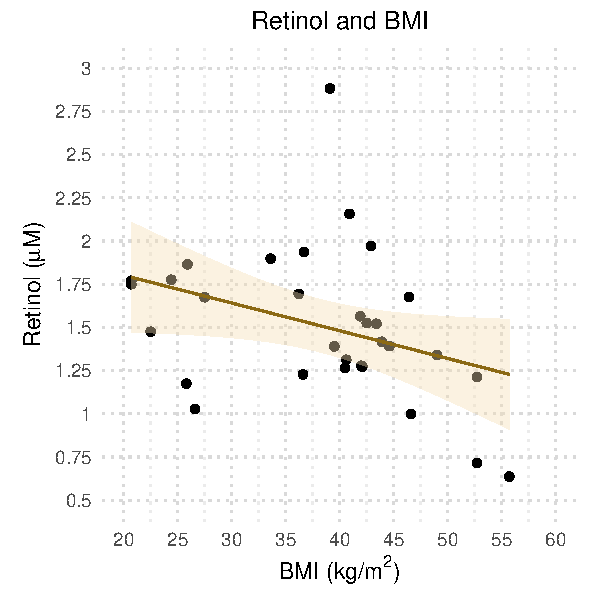
\includegraphics{StatisticalAnalysis_files/figure-latex/retinol plots-1.pdf}

\newpage

\subsection{Sensitivity Analysis of Retinol and
BMI}\label{sensitivity-analysis-of-retinol-and-bmi}

\begin{Shaded}
\begin{Highlighting}[]
\NormalTok{vaono23 }\OtherTok{\textless{}{-}}\NormalTok{vao }\SpecialCharTok{\%\textgreater{}\%} \FunctionTok{filter}\NormalTok{(ID}\SpecialCharTok{!=} \StringTok{"51{-}3523"}\NormalTok{) }\CommentTok{\#omit 23 from data set}
\NormalTok{Rmodel12no23}\OtherTok{\textless{}{-}}\FunctionTok{lm}\NormalTok{(LROL}\SpecialCharTok{\textasciitilde{}}\NormalTok{BMI,vaono23)}
\FunctionTok{summary}\NormalTok{(Rmodel12no23)}
\end{Highlighting}
\end{Shaded}

\begin{verbatim}
## 
## Call:
## lm(formula = LROL ~ BMI, data = vaono23)
## 
## Residuals:
##       Min        1Q    Median        3Q       Max 
## -0.258376 -0.049593  0.003565  0.047807  0.293192 
## 
## Coefficients:
##              Estimate Std. Error t value Pr(>|t|)    
## (Intercept)  0.321821   0.086169   3.735 0.000852 ***
## BMI         -0.003968   0.002226  -1.783 0.085468 .  
## ---
## Signif. codes:  0 '***' 0.001 '**' 0.01 '*' 0.05 '.' 0.1 ' ' 1
## 
## Residual standard error: 0.1114 on 28 degrees of freedom
## Multiple R-squared:  0.1019, Adjusted R-squared:  0.06987 
## F-statistic: 3.178 on 1 and 28 DF,  p-value: 0.08547
\end{verbatim}

\begin{quote}
Omission of participant with liver fibrosis and overt retinol deficiency
from the regression model increased the p-value of correlation between
BMI and retinol to p=0.09
\end{quote}

\subsection{Retinol Regressions Omitting Participant with Retinol
Deficiency and Apparent Liver
Fibrosis}\label{retinol-regressions-omitting-participant-with-retinol-deficiency-and-apparent-liver-fibrosis}

\begin{Shaded}
\begin{Highlighting}[]
\NormalTok{Rno23model1}\OtherTok{=}\FunctionTok{lm}\NormalTok{(LROL}\SpecialCharTok{\textasciitilde{}}\NormalTok{BMI}\SpecialCharTok{+}\NormalTok{Sex}\SpecialCharTok{+}\NormalTok{Age}\SpecialCharTok{+}\NormalTok{LHOMAIR,vaono23)}
\FunctionTok{summary}\NormalTok{(Rno23model1)}
\end{Highlighting}
\end{Shaded}

\begin{verbatim}
## 
## Call:
## lm(formula = LROL ~ BMI + Sex + Age + LHOMAIR, data = vaono23)
## 
## Residuals:
##       Min        1Q    Median        3Q       Max 
## -0.255391 -0.062874 -0.002688  0.052888  0.230952 
## 
## Coefficients:
##               Estimate Std. Error t value Pr(>|t|)
## (Intercept)  0.0639189  0.1612890   0.396    0.695
## BMI         -0.0008989  0.0027014  -0.333    0.742
## SexMale      0.0677670  0.0466130   1.454    0.158
## Age          0.0028660  0.0021708   1.320    0.199
## LHOMAIR     -0.0193169  0.0420587  -0.459    0.650
## 
## Residual standard error: 0.1092 on 25 degrees of freedom
## Multiple R-squared:  0.2294, Adjusted R-squared:  0.1061 
## F-statistic:  1.86 on 4 and 25 DF,  p-value: 0.1489
\end{verbatim}

\begin{Shaded}
\begin{Highlighting}[]
\CommentTok{\#remove one variable at a time}
\NormalTok{Rno23model2}\OtherTok{=}\FunctionTok{lm}\NormalTok{(LROL}\SpecialCharTok{\textasciitilde{}}\NormalTok{BMI}\SpecialCharTok{+}\NormalTok{Sex}\SpecialCharTok{+}\NormalTok{Age,vaono23) }\CommentTok{\#remove HOMAIR}
\NormalTok{Rno23model3}\OtherTok{=}\FunctionTok{lm}\NormalTok{(LROL}\SpecialCharTok{\textasciitilde{}}\NormalTok{BMI}\SpecialCharTok{+}\NormalTok{Sex}\SpecialCharTok{+}\NormalTok{LHOMAIR, vaono23) }\CommentTok{\#remove Age}
\NormalTok{Rno23model4}\OtherTok{=}\FunctionTok{lm}\NormalTok{(LROL}\SpecialCharTok{\textasciitilde{}}\NormalTok{BMI}\SpecialCharTok{+}\NormalTok{Age}\SpecialCharTok{+}\NormalTok{LHOMAIR, vaono23) }\CommentTok{\#remove Sex}
\NormalTok{Rno23model5}\OtherTok{=}\FunctionTok{lm}\NormalTok{(LROL}\SpecialCharTok{\textasciitilde{}}\NormalTok{Sex}\SpecialCharTok{+}\NormalTok{Age}\SpecialCharTok{+}\NormalTok{LHOMAIR, vaono23) }\CommentTok{\#remove BMI}

\NormalTok{AICR}\OtherTok{\textless{}{-}}\FunctionTok{AIC}\NormalTok{(Rno23model1, Rno23model2, Rno23model3, Rno23model4,Rno23model5) }\CommentTok{\#summary of AIC}
\NormalTok{AICR\_df}\OtherTok{\textless{}{-}}\FunctionTok{data.frame}\NormalTok{(}
  \AttributeTok{Model=}\FunctionTok{c}\NormalTok{(}\StringTok{"Model 1: Full Model"}\NormalTok{, }\StringTok{"Model 2: No HOMA{-}IR"}\NormalTok{, }\StringTok{"Model 3: No Age"}\NormalTok{, }
          \StringTok{"Model 4: No Sex"}\NormalTok{, }\StringTok{"Model 5: No BMI"}\NormalTok{),}
  \AttributeTok{AIC =}\NormalTok{ AICR}\SpecialCharTok{$}\NormalTok{AIC,}
  \AttributeTok{DF =}\NormalTok{ AICR}\SpecialCharTok{$}\NormalTok{df)}
\NormalTok{aicR\_table }\OtherTok{\textless{}{-}}\NormalTok{ AICR\_df }\SpecialCharTok{\%\textgreater{}\%}
  \FunctionTok{flextable}\NormalTok{() }\SpecialCharTok{\%\textgreater{}\%}
  \FunctionTok{set\_header\_labels}\NormalTok{(}\AttributeTok{Model =} \StringTok{"Model Description"}\NormalTok{, }\AttributeTok{AIC =} \StringTok{"AIC Value"}\NormalTok{,}
                    \AttributeTok{DF=}\StringTok{"Degrees of Freedom"}\NormalTok{) }\SpecialCharTok{\%\textgreater{}\%}
  \FunctionTok{add\_header\_lines}\NormalTok{(}\AttributeTok{values =} \StringTok{"AIC Comparison of Models for Retinol (Omitting 23)"}\NormalTok{) }\SpecialCharTok{\%\textgreater{}\%}
  \FunctionTok{align}\NormalTok{(}\AttributeTok{part=}\StringTok{"header"}\NormalTok{, }\AttributeTok{align=}\StringTok{"center"}\NormalTok{ ) }\SpecialCharTok{\%\textgreater{}\%}
  \FunctionTok{add\_footer\_lines}\NormalTok{(}\AttributeTok{values =} \StringTok{"Note: Lower AIC values indicate a better model."}\NormalTok{) }\SpecialCharTok{\%\textgreater{}\%}
  \FunctionTok{fontsize}\NormalTok{(}\AttributeTok{part =} \StringTok{"footer"}\NormalTok{, }\AttributeTok{size =} \DecValTok{8}\NormalTok{) }\SpecialCharTok{\%\textgreater{}\%}
  \FunctionTok{set\_table\_properties}\NormalTok{(}\AttributeTok{layout =} \StringTok{"autofit"}\NormalTok{)}
\NormalTok{aicR\_table}
\end{Highlighting}
\end{Shaded}

\global\setlength{\Oldarrayrulewidth}{\arrayrulewidth}

\global\setlength{\Oldtabcolsep}{\tabcolsep}

\setlength{\tabcolsep}{2pt}

\renewcommand*{\arraystretch}{1.5}



\providecommand{\ascline}[3]{\noalign{\global\arrayrulewidth #1}\arrayrulecolor[HTML]{#2}\cline{#3}}

\begin{longtable}[c]{ccc}



\ascline{1.5pt}{666666}{1-3}

\multicolumn{3}{>{}c}{\textcolor[HTML]{000000}{\fontsize{11}{11}\selectfont{\global\setmainfont{Arial}{AIC\ Comparison\ of\ Models\ for\ Retinol\ (Omitting\ 23)}}}} \\

\ascline{1.5pt}{666666}{1-3}



\multicolumn{1}{>{}c}{\textcolor[HTML]{000000}{\fontsize{11}{11}\selectfont{\global\setmainfont{Arial}{Model\ Description}}}} & \multicolumn{1}{>{}c}{\textcolor[HTML]{000000}{\fontsize{11}{11}\selectfont{\global\setmainfont{Arial}{AIC\ Value}}}} & \multicolumn{1}{>{}c}{\textcolor[HTML]{000000}{\fontsize{11}{11}\selectfont{\global\setmainfont{Arial}{Degrees\ of\ Freedom}}}} \\

\ascline{1.5pt}{666666}{1-3}\endfirsthead 

\ascline{1.5pt}{666666}{1-3}

\multicolumn{3}{>{}c}{\textcolor[HTML]{000000}{\fontsize{11}{11}\selectfont{\global\setmainfont{Arial}{AIC\ Comparison\ of\ Models\ for\ Retinol\ (Omitting\ 23)}}}} \\

\ascline{1.5pt}{666666}{1-3}



\multicolumn{1}{>{}c}{\textcolor[HTML]{000000}{\fontsize{11}{11}\selectfont{\global\setmainfont{Arial}{Model\ Description}}}} & \multicolumn{1}{>{}c}{\textcolor[HTML]{000000}{\fontsize{11}{11}\selectfont{\global\setmainfont{Arial}{AIC\ Value}}}} & \multicolumn{1}{>{}c}{\textcolor[HTML]{000000}{\fontsize{11}{11}\selectfont{\global\setmainfont{Arial}{Degrees\ of\ Freedom}}}} \\

\ascline{1.5pt}{666666}{1-3}\endhead



\multicolumn{3}{>{}l}{\textcolor[HTML]{000000}{\fontsize{8}{8}\selectfont{\global\setmainfont{Arial}{Note:\ Lower\ AIC\ values\ indicate\ a\ better\ model.}}}} \\

\endlastfoot



\multicolumn{1}{>{}l}{\textcolor[HTML]{000000}{\fontsize{11}{11}\selectfont{\global\setmainfont{Arial}{Model\ 1:\ Full\ Model}}}} & \multicolumn{1}{>{}r}{\textcolor[HTML]{000000}{\fontsize{11}{11}\selectfont{\global\setmainfont{Arial}{-41.21348}}}} & \multicolumn{1}{>{}r}{\textcolor[HTML]{000000}{\fontsize{11}{11}\selectfont{\global\setmainfont{Arial}{6}}}} \\





\multicolumn{1}{>{}l}{\textcolor[HTML]{000000}{\fontsize{11}{11}\selectfont{\global\setmainfont{Arial}{Model\ 2:\ No\ HOMA-IR}}}} & \multicolumn{1}{>{}r}{\textcolor[HTML]{000000}{\fontsize{11}{11}\selectfont{\global\setmainfont{Arial}{-42.96142}}}} & \multicolumn{1}{>{}r}{\textcolor[HTML]{000000}{\fontsize{11}{11}\selectfont{\global\setmainfont{Arial}{5}}}} \\





\multicolumn{1}{>{}l}{\textcolor[HTML]{000000}{\fontsize{11}{11}\selectfont{\global\setmainfont{Arial}{Model\ 3:\ No\ Age}}}} & \multicolumn{1}{>{}r}{\textcolor[HTML]{000000}{\fontsize{11}{11}\selectfont{\global\setmainfont{Arial}{-41.19143}}}} & \multicolumn{1}{>{}r}{\textcolor[HTML]{000000}{\fontsize{11}{11}\selectfont{\global\setmainfont{Arial}{5}}}} \\





\multicolumn{1}{>{}l}{\textcolor[HTML]{000000}{\fontsize{11}{11}\selectfont{\global\setmainfont{Arial}{Model\ 4:\ No\ Sex}}}} & \multicolumn{1}{>{}r}{\textcolor[HTML]{000000}{\fontsize{11}{11}\selectfont{\global\setmainfont{Arial}{-40.77869}}}} & \multicolumn{1}{>{}r}{\textcolor[HTML]{000000}{\fontsize{11}{11}\selectfont{\global\setmainfont{Arial}{5}}}} \\





\multicolumn{1}{>{}l}{\textcolor[HTML]{000000}{\fontsize{11}{11}\selectfont{\global\setmainfont{Arial}{Model\ 5:\ No\ BMI}}}} & \multicolumn{1}{>{}r}{\textcolor[HTML]{000000}{\fontsize{11}{11}\selectfont{\global\setmainfont{Arial}{-43.08092}}}} & \multicolumn{1}{>{}r}{\textcolor[HTML]{000000}{\fontsize{11}{11}\selectfont{\global\setmainfont{Arial}{5}}}} \\

\ascline{1.5pt}{666666}{1-3}



\end{longtable}



\arrayrulecolor[HTML]{000000}

\global\setlength{\arrayrulewidth}{\Oldarrayrulewidth}

\global\setlength{\tabcolsep}{\Oldtabcolsep}

\renewcommand*{\arraystretch}{1}

\begin{Shaded}
\begin{Highlighting}[]
\CommentTok{\#remove BMI, add interaction terms}
\NormalTok{Rno23model6}\OtherTok{=}\FunctionTok{lm}\NormalTok{(LROL}\SpecialCharTok{\textasciitilde{}}\NormalTok{Sex}\SpecialCharTok{+}\NormalTok{Age}\SpecialCharTok{+}\NormalTok{LHOMAIR}\SpecialCharTok{+}\NormalTok{Sex}\SpecialCharTok{*}\NormalTok{Age,vaono23)}
\NormalTok{Rno23model7}\OtherTok{=}\FunctionTok{lm}\NormalTok{(LROL}\SpecialCharTok{\textasciitilde{}}\NormalTok{Sex}\SpecialCharTok{+}\NormalTok{Age}\SpecialCharTok{+}\NormalTok{Sex}\SpecialCharTok{*}\NormalTok{Age,vaono23) }\CommentTok{\#remove HOMA}
\NormalTok{Rno23model8}\OtherTok{=}\FunctionTok{lm}\NormalTok{(LROL}\SpecialCharTok{\textasciitilde{}}\NormalTok{Sex}\SpecialCharTok{+}\NormalTok{Age,vaono23) }\CommentTok{\#remove HOMA and Sex * Age}
\NormalTok{Rno23model9}\OtherTok{=}\FunctionTok{lm}\NormalTok{(LROL}\SpecialCharTok{\textasciitilde{}}\NormalTok{Sex}\SpecialCharTok{+}\NormalTok{LHOMAIR,vaono23) }\CommentTok{\#remove Age}
\NormalTok{Rno23model10}\OtherTok{=}\FunctionTok{lm}\NormalTok{(LROL}\SpecialCharTok{\textasciitilde{}}\NormalTok{Age}\SpecialCharTok{+}\NormalTok{LHOMAIR,vaono23) }\CommentTok{\#remove Sex}

\FunctionTok{AIC}\NormalTok{(Rno23model5, Rno23model6,Rno23model7,Rno23model8,Rno23model9,Rno23model10)}
\end{Highlighting}
\end{Shaded}

\begin{longtable}[]{@{}lrr@{}}
\toprule\noalign{}
& df & AIC \\
\midrule\noalign{}
\endhead
\bottomrule\noalign{}
\endlastfoot
Rno23model5 & 5 & -43.08092 \\
Rno23model6 & 6 & -42.14048 \\
Rno23model7 & 5 & -43.85300 \\
Rno23model8 & 4 & -44.68606 \\
Rno23model9 & 4 & -42.70304 \\
Rno23model10 & 4 & -41.45723 \\
\end{longtable}

\begin{Shaded}
\begin{Highlighting}[]
\CommentTok{\#model 8 has the lowest AIC}
\CommentTok{\#Sex + Age}
\FunctionTok{summary}\NormalTok{(Rno23model8)}
\end{Highlighting}
\end{Shaded}

\begin{verbatim}
## 
## Call:
## lm(formula = LROL ~ Sex + Age, data = vaono23)
## 
## Residuals:
##      Min       1Q   Median       3Q      Max 
## -0.26566 -0.06596 -0.01165  0.04795  0.21500 
## 
## Coefficients:
##              Estimate Std. Error t value Pr(>|t|)  
## (Intercept) -0.004218   0.085347  -0.049   0.9609  
## SexMale      0.076579   0.040293   1.901   0.0681 .
## Age          0.003450   0.001926   1.791   0.0845 .
## ---
## Signif. codes:  0 '***' 0.001 '**' 0.01 '*' 0.05 '.' 0.1 ' ' 1
## 
## Residual standard error: 0.106 on 27 degrees of freedom
## Multiple R-squared:  0.2157, Adjusted R-squared:  0.1576 
## F-statistic: 3.713 on 2 and 27 DF,  p-value: 0.03763
\end{verbatim}

\begin{Shaded}
\begin{Highlighting}[]
\CommentTok{\#how does this compare to the predictors alone}
\NormalTok{Rno23model11}\OtherTok{=}\FunctionTok{lm}\NormalTok{(LROL}\SpecialCharTok{\textasciitilde{}}\NormalTok{Sex,vaono23) }\CommentTok{\#Sex alone}
\NormalTok{Rno23model12}\OtherTok{=}\FunctionTok{lm}\NormalTok{(LROL}\SpecialCharTok{\textasciitilde{}}\NormalTok{Age,vaono23) }\CommentTok{\#Age alone}
\FunctionTok{AIC}\NormalTok{(Rno23model8, Rno23model11, Rno23model12)}
\end{Highlighting}
\end{Shaded}

\begin{longtable}[]{@{}lrr@{}}
\toprule\noalign{}
& df & AIC \\
\midrule\noalign{}
\endhead
\bottomrule\noalign{}
\endlastfoot
Rno23model8 & 4 & -44.68606 \\
Rno23model11 & 3 & -43.31838 \\
Rno23model12 & 3 & -42.91924 \\
\end{longtable}

\begin{Shaded}
\begin{Highlighting}[]
\FunctionTok{anova}\NormalTok{(Rno23model8,Rno23model11) }\CommentTok{\#not better than Sex alone}
\end{Highlighting}
\end{Shaded}

\begin{longtable}[]{@{}rrrrrr@{}}
\toprule\noalign{}
Res.Df & RSS & Df & Sum of Sq & F & Pr(\textgreater F) \\
\midrule\noalign{}
\endhead
\bottomrule\noalign{}
\endlastfoot
27 & 0.3033459 & NA & NA & NA & NA \\
28 & 0.3393832 & -1 & -0.0360373 & 3.207581 & 0.0845163 \\
\end{longtable}

\begin{Shaded}
\begin{Highlighting}[]
\FunctionTok{anova}\NormalTok{(Rno23model8,Rno23model12) }\CommentTok{\#not better than Age alone}
\end{Highlighting}
\end{Shaded}

\begin{longtable}[]{@{}rrrrrr@{}}
\toprule\noalign{}
Res.Df & RSS & Df & Sum of Sq & F & Pr(\textgreater F) \\
\midrule\noalign{}
\endhead
\bottomrule\noalign{}
\endlastfoot
27 & 0.3033459 & NA & NA & NA & NA \\
28 & 0.3439287 & -1 & -0.0405828 & 3.612165 & 0.0680846 \\
\end{longtable}

\begin{Shaded}
\begin{Highlighting}[]
\FunctionTok{summary}\NormalTok{(Rno23model11) }\CommentTok{\#p\textgreater{}0.05}
\end{Highlighting}
\end{Shaded}

\begin{verbatim}
## 
## Call:
## lm(formula = LROL ~ Sex, data = vaono23)
## 
## Residuals:
##       Min        1Q    Median        3Q       Max 
## -0.287994 -0.050487  0.001027  0.044673  0.235073 
## 
## Coefficients:
##             Estimate Std. Error t value Pr(>|t|)    
## (Intercept)  0.14230    0.02526   5.634 4.92e-06 ***
## SexMale      0.08247    0.04171   1.977   0.0579 .  
## ---
## Signif. codes:  0 '***' 0.001 '**' 0.01 '*' 0.05 '.' 0.1 ' ' 1
## 
## Residual standard error: 0.1101 on 28 degrees of freedom
## Multiple R-squared:  0.1225, Adjusted R-squared:  0.09117 
## F-statistic: 3.909 on 1 and 28 DF,  p-value: 0.05794
\end{verbatim}

\begin{Shaded}
\begin{Highlighting}[]
\FunctionTok{summary}\NormalTok{(Rno23model12) }\CommentTok{\#p\textgreater{}0.05}
\end{Highlighting}
\end{Shaded}

\begin{verbatim}
## 
## Call:
## lm(formula = LROL ~ Age, data = vaono23)
## 
## Residuals:
##       Min        1Q    Median        3Q       Max 
## -0.291619 -0.052172  0.005761  0.063472  0.261440 
## 
## Coefficients:
##             Estimate Std. Error t value Pr(>|t|)  
## (Intercept) 0.010978   0.088847   0.124   0.9025  
## Age         0.003749   0.002007   1.868   0.0723 .
## ---
## Signif. codes:  0 '***' 0.001 '**' 0.01 '*' 0.05 '.' 0.1 ' ' 1
## 
## Residual standard error: 0.1108 on 28 degrees of freedom
## Multiple R-squared:  0.1108, Adjusted R-squared:  0.079 
## F-statistic: 3.488 on 1 and 28 DF,  p-value: 0.07233
\end{verbatim}

\begin{Shaded}
\begin{Highlighting}[]
\FunctionTok{summary}\NormalTok{(}\FunctionTok{lm}\NormalTok{(LROL}\SpecialCharTok{\textasciitilde{}}\NormalTok{BMI,vaono23)) }
\end{Highlighting}
\end{Shaded}

\begin{verbatim}
## 
## Call:
## lm(formula = LROL ~ BMI, data = vaono23)
## 
## Residuals:
##       Min        1Q    Median        3Q       Max 
## -0.258376 -0.049593  0.003565  0.047807  0.293192 
## 
## Coefficients:
##              Estimate Std. Error t value Pr(>|t|)    
## (Intercept)  0.321821   0.086169   3.735 0.000852 ***
## BMI         -0.003968   0.002226  -1.783 0.085468 .  
## ---
## Signif. codes:  0 '***' 0.001 '**' 0.01 '*' 0.05 '.' 0.1 ' ' 1
## 
## Residual standard error: 0.1114 on 28 degrees of freedom
## Multiple R-squared:  0.1019, Adjusted R-squared:  0.06987 
## F-statistic: 3.178 on 1 and 28 DF,  p-value: 0.08547
\end{verbatim}

\begin{quote}
No significant correlates for retinol after omission participant with
gross morphology of liver fibrosis and overt retinol deficiency
\end{quote}

\newpage

\section{Genotype effect on Retinol, RBP4, and
TTR}\label{genotype-effect-on-retinol-rbp4-and-ttr}

\global\setlength{\Oldarrayrulewidth}{\arrayrulewidth}

\global\setlength{\Oldtabcolsep}{\tabcolsep}

\setlength{\tabcolsep}{2pt}

\renewcommand*{\arraystretch}{1.5}



\providecommand{\ascline}[3]{\noalign{\global\arrayrulewidth #1}\arrayrulecolor[HTML]{#2}\cline{#3}}

\begin{longtable}[c]{ccc}



\ascline{1.5pt}{666666}{1-3}

\multicolumn{3}{>{}c}{\textcolor[HTML]{000000}{\fontsize{11}{11}\selectfont{\global\setmainfont{Arial}{ANOVA\ Results\ Table}}}} \\

\ascline{1.5pt}{666666}{1-3}



\multicolumn{1}{>{}c}{\textcolor[HTML]{000000}{\fontsize{11}{11}\selectfont{\global\setmainfont{Arial}{Analyte}}}} & \multicolumn{1}{>{}c}{\textcolor[HTML]{000000}{\fontsize{11}{11}\selectfont{\global\setmainfont{Arial}{SNP}}}} & \multicolumn{1}{>{}c}{\textcolor[HTML]{000000}{\fontsize{11}{11}\selectfont{\global\setmainfont{Arial}{p-value}}}} \\

\ascline{1.5pt}{666666}{1-3}\endfirsthead 

\ascline{1.5pt}{666666}{1-3}

\multicolumn{3}{>{}c}{\textcolor[HTML]{000000}{\fontsize{11}{11}\selectfont{\global\setmainfont{Arial}{ANOVA\ Results\ Table}}}} \\

\ascline{1.5pt}{666666}{1-3}



\multicolumn{1}{>{}c}{\textcolor[HTML]{000000}{\fontsize{11}{11}\selectfont{\global\setmainfont{Arial}{Analyte}}}} & \multicolumn{1}{>{}c}{\textcolor[HTML]{000000}{\fontsize{11}{11}\selectfont{\global\setmainfont{Arial}{SNP}}}} & \multicolumn{1}{>{}c}{\textcolor[HTML]{000000}{\fontsize{11}{11}\selectfont{\global\setmainfont{Arial}{p-value}}}} \\

\ascline{1.5pt}{666666}{1-3}\endhead



\multicolumn{1}{>{}l}{\textcolor[HTML]{000000}{\fontsize{11}{11}\selectfont{\global\setmainfont{Arial}{Retinol}}}} & \multicolumn{1}{>{}l}{\textcolor[HTML]{000000}{\fontsize{11}{11}\selectfont{\global\setmainfont{Arial}{TTRsnp}}}} & \multicolumn{1}{>{}r}{\textcolor[HTML]{000000}{\fontsize{11}{11}\selectfont{\global\setmainfont{Arial}{0.63}}}} \\





\multicolumn{1}{>{}l}{\textcolor[HTML]{000000}{\fontsize{11}{11}\selectfont{\global\setmainfont{Arial}{Retinol}}}} & \multicolumn{1}{>{}l}{\textcolor[HTML]{000000}{\fontsize{11}{11}\selectfont{\global\setmainfont{Arial}{RBP4snp}}}} & \multicolumn{1}{>{}r}{\textcolor[HTML]{000000}{\fontsize{11}{11}\selectfont{\global\setmainfont{Arial}{0.86}}}} \\





\multicolumn{1}{>{}l}{\textcolor[HTML]{000000}{\fontsize{11}{11}\selectfont{\global\setmainfont{Arial}{RBP4}}}} & \multicolumn{1}{>{}l}{\textcolor[HTML]{000000}{\fontsize{11}{11}\selectfont{\global\setmainfont{Arial}{TTRsnp}}}} & \multicolumn{1}{>{}r}{\textcolor[HTML]{000000}{\fontsize{11}{11}\selectfont{\global\setmainfont{Arial}{0.48}}}} \\





\multicolumn{1}{>{}l}{\textcolor[HTML]{000000}{\fontsize{11}{11}\selectfont{\global\setmainfont{Arial}{RBP4}}}} & \multicolumn{1}{>{}l}{\textcolor[HTML]{000000}{\fontsize{11}{11}\selectfont{\global\setmainfont{Arial}{RBP4snp}}}} & \multicolumn{1}{>{}r}{\textcolor[HTML]{000000}{\fontsize{11}{11}\selectfont{\global\setmainfont{Arial}{0.70}}}} \\





\multicolumn{1}{>{}l}{\textcolor[HTML]{000000}{\fontsize{11}{11}\selectfont{\global\setmainfont{Arial}{TTR}}}} & \multicolumn{1}{>{}l}{\textcolor[HTML]{000000}{\fontsize{11}{11}\selectfont{\global\setmainfont{Arial}{TTRsnp}}}} & \multicolumn{1}{>{}r}{\textcolor[HTML]{000000}{\fontsize{11}{11}\selectfont{\global\setmainfont{Arial}{0.64}}}} \\





\multicolumn{1}{>{}l}{\textcolor[HTML]{000000}{\fontsize{11}{11}\selectfont{\global\setmainfont{Arial}{TTR}}}} & \multicolumn{1}{>{}l}{\textcolor[HTML]{000000}{\fontsize{11}{11}\selectfont{\global\setmainfont{Arial}{RBP4snp}}}} & \multicolumn{1}{>{}r}{\textcolor[HTML]{000000}{\fontsize{11}{11}\selectfont{\global\setmainfont{Arial}{0.36}}}} \\

\ascline{1.5pt}{666666}{1-3}



\end{longtable}



\arrayrulecolor[HTML]{000000}

\global\setlength{\arrayrulewidth}{\Oldarrayrulewidth}

\global\setlength{\tabcolsep}{\Oldtabcolsep}

\renewcommand*{\arraystretch}{1}

\section{Table S2, S3}\label{table-s2-s3}

\global\setlength{\Oldarrayrulewidth}{\arrayrulewidth}

\global\setlength{\Oldtabcolsep}{\tabcolsep}

\setlength{\tabcolsep}{2pt}

\renewcommand*{\arraystretch}{1.5}



\providecommand{\ascline}[3]{\noalign{\global\arrayrulewidth #1}\arrayrulecolor[HTML]{#2}\cline{#3}}

\begin{longtable}[c]{|p{0.95in}|p{1.41in}|p{1.66in}|p{1.41in}}



\ascline{1.5pt}{666666}{1-4}

\multicolumn{4}{>{\centering}m{\dimexpr 5.42in+6\tabcolsep}}{\textcolor[HTML]{000000}{\fontsize{11}{11}\selectfont{\global\setmainfont{Arial}{Analyte\ Conc.\ Stratified\ by\ }}}\textcolor[HTML]{000000}{\fontsize{11}{11}\selectfont{\global\setmainfont{Arial}{\textit{RBP4}}}}\textcolor[HTML]{000000}{\fontsize{11}{11}\selectfont{\global\setmainfont{Arial}{\ Genotype\ (rs10882272)}}}} \\

\ascline{1.5pt}{666666}{1-4}



\multicolumn{1}{>{\centering}m{\dimexpr 0.95in+0\tabcolsep}}{\textcolor[HTML]{000000}{\fontsize{11}{11}\selectfont{\global\setmainfont{Arial}{Genotype}}}} & \multicolumn{1}{>{\centering}m{\dimexpr 1.41in+0\tabcolsep}}{\textcolor[HTML]{000000}{\fontsize{11}{11}\selectfont{\global\setmainfont{Arial}{RBP4\ (μM)}}}} & \multicolumn{1}{>{\centering}m{\dimexpr 1.66in+0\tabcolsep}}{\textcolor[HTML]{000000}{\fontsize{11}{11}\selectfont{\global\setmainfont{Arial}{TTR\ (μM)}}}} & \multicolumn{1}{>{\centering}m{\dimexpr 1.41in+0\tabcolsep}}{\textcolor[HTML]{000000}{\fontsize{11}{11}\selectfont{\global\setmainfont{Arial}{Retinol\ (μM)}}}} \\

\ascline{1.5pt}{666666}{1-4}\endfirsthead 

\ascline{1.5pt}{666666}{1-4}

\multicolumn{4}{>{\centering}m{\dimexpr 5.42in+6\tabcolsep}}{\textcolor[HTML]{000000}{\fontsize{11}{11}\selectfont{\global\setmainfont{Arial}{Analyte\ Conc.\ Stratified\ by\ }}}\textcolor[HTML]{000000}{\fontsize{11}{11}\selectfont{\global\setmainfont{Arial}{\textit{RBP4}}}}\textcolor[HTML]{000000}{\fontsize{11}{11}\selectfont{\global\setmainfont{Arial}{\ Genotype\ (rs10882272)}}}} \\

\ascline{1.5pt}{666666}{1-4}



\multicolumn{1}{>{\centering}m{\dimexpr 0.95in+0\tabcolsep}}{\textcolor[HTML]{000000}{\fontsize{11}{11}\selectfont{\global\setmainfont{Arial}{Genotype}}}} & \multicolumn{1}{>{\centering}m{\dimexpr 1.41in+0\tabcolsep}}{\textcolor[HTML]{000000}{\fontsize{11}{11}\selectfont{\global\setmainfont{Arial}{RBP4\ (μM)}}}} & \multicolumn{1}{>{\centering}m{\dimexpr 1.66in+0\tabcolsep}}{\textcolor[HTML]{000000}{\fontsize{11}{11}\selectfont{\global\setmainfont{Arial}{TTR\ (μM)}}}} & \multicolumn{1}{>{\centering}m{\dimexpr 1.41in+0\tabcolsep}}{\textcolor[HTML]{000000}{\fontsize{11}{11}\selectfont{\global\setmainfont{Arial}{Retinol\ (μM)}}}} \\

\ascline{1.5pt}{666666}{1-4}\endhead



\multicolumn{4}{>{\raggedright}m{\dimexpr 5.42in+6\tabcolsep}}{\textcolor[HTML]{000000}{\fontsize{9}{9}\selectfont{\global\setmainfont{Arial}{Concentrations\ shown\ as\ geometric\ mean\ and\ range}}}} \\





\multicolumn{4}{>{\raggedright}m{\dimexpr 5.42in+6\tabcolsep}}{\textcolor[HTML]{000000}{\fontsize{9}{9}\selectfont{\global\setmainfont{Arial}{For\ the\ }}}\textcolor[HTML]{000000}{\fontsize{9}{9}\selectfont{\global\setmainfont{Arial}{\textit{RBP4}}}}\textcolor[HTML]{000000}{\fontsize{9}{9}\selectfont{\global\setmainfont{Arial}{\ genotype,\ 1/1\ refers\ to\ T/T,\ 1/2\ to\ T/C\ and\ 2/2\ to\ C/C\ for\ single\ nucleotide\ polymorphism\ in\ the\ 3’\ untranslated\ region}}}} \\

\endlastfoot



\multicolumn{1}{>{\raggedright}m{\dimexpr 0.95in+0\tabcolsep}}{\textcolor[HTML]{000000}{\fontsize{11}{11}\selectfont{\global\setmainfont{Arial}{\ 1/1}}}} & \multicolumn{1}{>{\raggedright}m{\dimexpr 1.41in+0\tabcolsep}}{\textcolor[HTML]{000000}{\fontsize{11}{11}\selectfont{\global\setmainfont{Arial}{1.91\ (1.00,\ 3.16)}}}} & \multicolumn{1}{>{\raggedright}m{\dimexpr 1.66in+0\tabcolsep}}{\textcolor[HTML]{000000}{\fontsize{11}{11}\selectfont{\global\setmainfont{Arial}{19.20\ (10.37,\ 26.61)}}}} & \multicolumn{1}{>{\raggedright}m{\dimexpr 1.41in+0\tabcolsep}}{\textcolor[HTML]{000000}{\fontsize{11}{11}\selectfont{\global\setmainfont{Arial}{1.35\ (0.71,\ 2.88)}}}} \\





\multicolumn{1}{>{\raggedright}m{\dimexpr 0.95in+0\tabcolsep}}{\textcolor[HTML]{000000}{\fontsize{11}{11}\selectfont{\global\setmainfont{Arial}{\ 1/2}}}} & \multicolumn{1}{>{\raggedright}m{\dimexpr 1.41in+0\tabcolsep}}{\textcolor[HTML]{000000}{\fontsize{11}{11}\selectfont{\global\setmainfont{Arial}{2.15\ (1.19,\ 3.24)}}}} & \multicolumn{1}{>{\raggedright}m{\dimexpr 1.66in+0\tabcolsep}}{\textcolor[HTML]{000000}{\fontsize{11}{11}\selectfont{\global\setmainfont{Arial}{21.27\ (13.07,\ 29.81)}}}} & \multicolumn{1}{>{\raggedright}m{\dimexpr 1.41in+0\tabcolsep}}{\textcolor[HTML]{000000}{\fontsize{11}{11}\selectfont{\global\setmainfont{Arial}{1.52\ (1.00,\ 2.16)}}}} \\





\multicolumn{1}{>{\raggedright}m{\dimexpr 0.95in+0\tabcolsep}}{\textcolor[HTML]{000000}{\fontsize{11}{11}\selectfont{\global\setmainfont{Arial}{\ 2/2}}}} & \multicolumn{1}{>{\raggedright}m{\dimexpr 1.41in+0\tabcolsep}}{\textcolor[HTML]{000000}{\fontsize{11}{11}\selectfont{\global\setmainfont{Arial}{2.10\ (0.95,\ 3.18)}}}} & \multicolumn{1}{>{\raggedright}m{\dimexpr 1.66in+0\tabcolsep}}{\textcolor[HTML]{000000}{\fontsize{11}{11}\selectfont{\global\setmainfont{Arial}{20.24\ (12.03,\ 29.55)}}}} & \multicolumn{1}{>{\raggedright}m{\dimexpr 1.41in+0\tabcolsep}}{\textcolor[HTML]{000000}{\fontsize{11}{11}\selectfont{\global\setmainfont{Arial}{1.42\ (0.64,\ 1.97)}}}} \\

\ascline{1.5pt}{666666}{1-4}



\end{longtable}



\arrayrulecolor[HTML]{000000}

\global\setlength{\arrayrulewidth}{\Oldarrayrulewidth}

\global\setlength{\tabcolsep}{\Oldtabcolsep}

\renewcommand*{\arraystretch}{1}

\global\setlength{\Oldarrayrulewidth}{\arrayrulewidth}

\global\setlength{\Oldtabcolsep}{\tabcolsep}

\setlength{\tabcolsep}{2pt}

\renewcommand*{\arraystretch}{1.5}



\providecommand{\ascline}[3]{\noalign{\global\arrayrulewidth #1}\arrayrulecolor[HTML]{#2}\cline{#3}}

\begin{longtable}[c]{|p{0.95in}|p{1.41in}|p{1.66in}|p{1.41in}}



\ascline{1.5pt}{666666}{1-4}

\multicolumn{4}{>{\centering}m{\dimexpr 5.42in+6\tabcolsep}}{\textcolor[HTML]{000000}{\fontsize{11}{11}\selectfont{\global\setmainfont{Arial}{Analyte\ Conc.\ Stratified\ by\ }}}\textcolor[HTML]{000000}{\fontsize{11}{11}\selectfont{\global\setmainfont{Arial}{\textit{TTR}}}}\textcolor[HTML]{000000}{\fontsize{11}{11}\selectfont{\global\setmainfont{Arial}{\ Genotype\ (rs1667255)}}}} \\

\ascline{1.5pt}{666666}{1-4}



\multicolumn{1}{>{\centering}m{\dimexpr 0.95in+0\tabcolsep}}{\textcolor[HTML]{000000}{\fontsize{11}{11}\selectfont{\global\setmainfont{Arial}{Genotype}}}} & \multicolumn{1}{>{\centering}m{\dimexpr 1.41in+0\tabcolsep}}{\textcolor[HTML]{000000}{\fontsize{11}{11}\selectfont{\global\setmainfont{Arial}{RBP4\ (μM)}}}} & \multicolumn{1}{>{\centering}m{\dimexpr 1.66in+0\tabcolsep}}{\textcolor[HTML]{000000}{\fontsize{11}{11}\selectfont{\global\setmainfont{Arial}{TTR\ (μM)}}}} & \multicolumn{1}{>{\centering}m{\dimexpr 1.41in+0\tabcolsep}}{\textcolor[HTML]{000000}{\fontsize{11}{11}\selectfont{\global\setmainfont{Arial}{Retinol\ (μM)}}}} \\

\ascline{1.5pt}{666666}{1-4}\endfirsthead 

\ascline{1.5pt}{666666}{1-4}

\multicolumn{4}{>{\centering}m{\dimexpr 5.42in+6\tabcolsep}}{\textcolor[HTML]{000000}{\fontsize{11}{11}\selectfont{\global\setmainfont{Arial}{Analyte\ Conc.\ Stratified\ by\ }}}\textcolor[HTML]{000000}{\fontsize{11}{11}\selectfont{\global\setmainfont{Arial}{\textit{TTR}}}}\textcolor[HTML]{000000}{\fontsize{11}{11}\selectfont{\global\setmainfont{Arial}{\ Genotype\ (rs1667255)}}}} \\

\ascline{1.5pt}{666666}{1-4}



\multicolumn{1}{>{\centering}m{\dimexpr 0.95in+0\tabcolsep}}{\textcolor[HTML]{000000}{\fontsize{11}{11}\selectfont{\global\setmainfont{Arial}{Genotype}}}} & \multicolumn{1}{>{\centering}m{\dimexpr 1.41in+0\tabcolsep}}{\textcolor[HTML]{000000}{\fontsize{11}{11}\selectfont{\global\setmainfont{Arial}{RBP4\ (μM)}}}} & \multicolumn{1}{>{\centering}m{\dimexpr 1.66in+0\tabcolsep}}{\textcolor[HTML]{000000}{\fontsize{11}{11}\selectfont{\global\setmainfont{Arial}{TTR\ (μM)}}}} & \multicolumn{1}{>{\centering}m{\dimexpr 1.41in+0\tabcolsep}}{\textcolor[HTML]{000000}{\fontsize{11}{11}\selectfont{\global\setmainfont{Arial}{Retinol\ (μM)}}}} \\

\ascline{1.5pt}{666666}{1-4}\endhead



\multicolumn{4}{>{\raggedright}m{\dimexpr 5.42in+6\tabcolsep}}{\textcolor[HTML]{000000}{\fontsize{9}{9}\selectfont{\global\setmainfont{Arial}{Concentrations\ shown\ as\ geometric\ mean\ and\ range}}}} \\





\multicolumn{4}{>{\raggedright}m{\dimexpr 5.42in+6\tabcolsep}}{\textcolor[HTML]{000000}{\fontsize{9}{9}\selectfont{\global\setmainfont{Arial}{For\ the\ }}}\textcolor[HTML]{000000}{\fontsize{9}{9}\selectfont{\global\setmainfont{Arial}{\textit{TTR}}}}\textcolor[HTML]{000000}{\fontsize{9}{9}\selectfont{\global\setmainfont{Arial}{\ genotype,\ 1/1\ refers\ to\ A/A,\ 1/2\ to\ A/C\ and\ 2/2\ to\ C/C\ for\ intronic\ single\ nucleotide\ polymorphism}}}} \\

\endlastfoot



\multicolumn{1}{>{\raggedright}m{\dimexpr 0.95in+0\tabcolsep}}{\textcolor[HTML]{000000}{\fontsize{11}{11}\selectfont{\global\setmainfont{Arial}{\ 1/1}}}} & \multicolumn{1}{>{\raggedright}m{\dimexpr 1.41in+0\tabcolsep}}{\textcolor[HTML]{000000}{\fontsize{11}{11}\selectfont{\global\setmainfont{Arial}{1.88\ (0.95,\ 3.16)}}}} & \multicolumn{1}{>{\raggedright}m{\dimexpr 1.66in+0\tabcolsep}}{\textcolor[HTML]{000000}{\fontsize{11}{11}\selectfont{\global\setmainfont{Arial}{18.84\ (12.03,\ 26.61)}}}} & \multicolumn{1}{>{\raggedright}m{\dimexpr 1.41in+0\tabcolsep}}{\textcolor[HTML]{000000}{\fontsize{11}{11}\selectfont{\global\setmainfont{Arial}{1.42\ (0.64,\ 2.88)}}}} \\





\multicolumn{1}{>{\raggedright}m{\dimexpr 0.95in+0\tabcolsep}}{\textcolor[HTML]{000000}{\fontsize{11}{11}\selectfont{\global\setmainfont{Arial}{\ 1/2}}}} & \multicolumn{1}{>{\raggedright}m{\dimexpr 1.41in+0\tabcolsep}}{\textcolor[HTML]{000000}{\fontsize{11}{11}\selectfont{\global\setmainfont{Arial}{2.10\ (1.00,\ 3.04)}}}} & \multicolumn{1}{>{\raggedright}m{\dimexpr 1.66in+0\tabcolsep}}{\textcolor[HTML]{000000}{\fontsize{11}{11}\selectfont{\global\setmainfont{Arial}{20.39\ (10.37,\ 29.81)}}}} & \multicolumn{1}{>{\raggedright}m{\dimexpr 1.41in+0\tabcolsep}}{\textcolor[HTML]{000000}{\fontsize{11}{11}\selectfont{\global\setmainfont{Arial}{1.38\ (0.71,\ 1.69)}}}} \\





\multicolumn{1}{>{\raggedright}m{\dimexpr 0.95in+0\tabcolsep}}{\textcolor[HTML]{000000}{\fontsize{11}{11}\selectfont{\global\setmainfont{Arial}{\ 2/2}}}} & \multicolumn{1}{>{\raggedright}m{\dimexpr 1.41in+0\tabcolsep}}{\textcolor[HTML]{000000}{\fontsize{11}{11}\selectfont{\global\setmainfont{Arial}{2.27\ (1.50,\ 3.24)}}}} & \multicolumn{1}{>{\raggedright}m{\dimexpr 1.66in+0\tabcolsep}}{\textcolor[HTML]{000000}{\fontsize{11}{11}\selectfont{\global\setmainfont{Arial}{22.27\ (16.46,\ 29.79)}}}} & \multicolumn{1}{>{\raggedright}m{\dimexpr 1.41in+0\tabcolsep}}{\textcolor[HTML]{000000}{\fontsize{11}{11}\selectfont{\global\setmainfont{Arial}{1.56\ (1.21,\ 2.16)}}}} \\

\ascline{1.5pt}{666666}{1-4}



\end{longtable}



\arrayrulecolor[HTML]{000000}

\global\setlength{\arrayrulewidth}{\Oldarrayrulewidth}

\global\setlength{\tabcolsep}{\Oldtabcolsep}

\renewcommand*{\arraystretch}{1}

\newpage

\section{Figure 2}\label{figure-2}

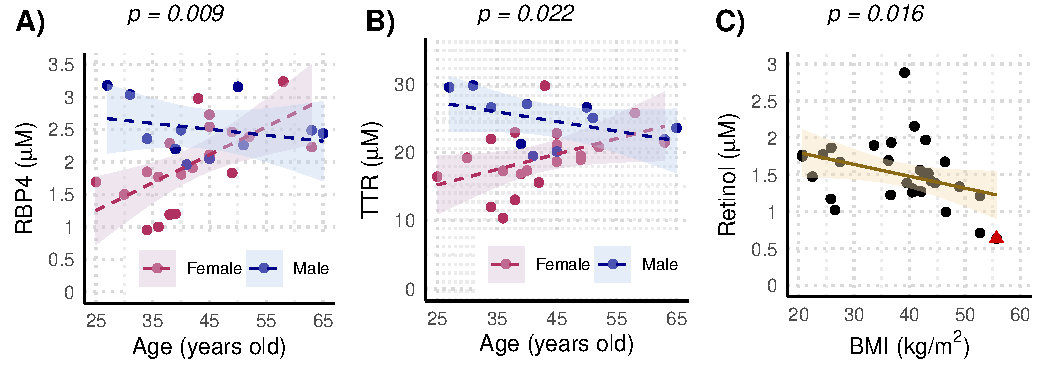
\includegraphics{StatisticalAnalysis_files/figure-latex/figure 2-1.pdf}

\end{document}
